% Steven Milan Moreno
% Thesis Version 1.0.0
% April 18th, 2024 (1.0.0)
% May 13th, 2024 (1.0.1)
% March 1st, 2025 (1.1.2)
% May 23rd, 2025 (1.1.3)
% July 7th, 2025 (1.1.4)
% July 14th, 2025 (1.1.5) CH2_DFT1_Complete 
% August 5th, 2025 (1.1.6)
% August 20th, 2025 (1.2.7) CH3_DFT1_Complete, CH2_DFT2(FB)_Complete
% September 1st, 2025 (1.2.8) CH1_DFT1_Complete
% September 9th, 2025 (1.2.9) CH6-7_DFT1_Complete
% September 16th, 2025 (1.2.10) CH4,5_Updated_Significantly
% September 29th, 2025 (1.3.11) CH1-5(FB) Complete
% October 6th, 2025 (1.3.12) CH4-6_Updated_Significantly
% October 14th, 2025 (1.4.12) TEXT COMPLETE
% October 20th, 2025 (1.4.13) Feedback Implemented
% Octover 25th, 2025 (1.5.14) Heavy Restrcuturing of Intro, Feedback Implemented
% October 28th, 2025 (2.0.0) Completed Restructuring of Into/End of All Chapters, Conclusion Modified


%Outline format based on template shared by John Davies <john.davies@glasgow.ac.uk> 2017-02-06
% It matches the university specification at the time of writing

%VerA.B.C
%A = Updated Entire/ Nearly Entire Draft After Feedback (Inner-Chapter Alterations) = +1
%B = Updated Section/Chapter After Feedback (Intra-Chapter Alteration)= +1
%C = Added 1st Draft Content, Minor Updates = +1

\documentclass[12pt,titlepage,oneside]{book}
\usepackage[T1]{fontenc} % modern encoding
% Comment out the next three lines of LaTeX if you wish to use Computer Modern fonts
%   (this is the default for LaTeX, easier for mathematics heavy papers)
\usepackage{float}
\usepackage{mathptmx}  
\usepackage[scaled]{helvet} 
\usepackage{courier} 
\usepackage{subcaption}
\usepackage[labelfont=bf]{caption}
\usepackage[font=small,labelfont=bf,margin=\parindent,tableposition=top]{caption}
\usepackage{graphicx}  
\usepackage{cite}  
\usepackage[top=1.8cm, bottom=1.8cm,left=4.0cm,right=1.5cm]{geometry}
\usepackage[onehalfspacing]{setspace} 
\usepackage{tikz}
\usepackage{gensymb}
\usepackage{lscape} 
\usepackage{pgfplots}
\usepackage{tikzviolinplots}
\usepackage{filecontents}
\usepackage{datatool}
\usepackage{booktabs}
\usepackage{longtable}
\usepackage{array}



\usetikzlibrary{shapes, arrows}
\pgfplotsset{compat=1.18}
\pgfplotsset{empty line = none}
\usepgfplotslibrary{statistics}
%\usepgfplotslibrary{external} 
%\tikzexternalize

\begin{document}
\begin{titlepage}
\centering
\vspace*{3cm}  % Need the * or the space is swallowed at the top of the page
\bfseries\Large
Optimized Pipeline For Clearing, Mounting, and Mesoscale Imaging of Leporine Cardiac Tissue Structure\\


\vspace{1.5cm}
**COMPLETE DRAFT**\\
Version 1.4.12\\
\vspace{1.5cm}
\normalfont\large
Steven Milan Moreno\\
\vspace{2cm}
Submitted in fulfilment of the requirements for the\\
Degree of Doctor of Philosophy\\
\vspace{2cm}
School of Physics and Astronomy\\
College of Science and Engineering\\
University of Glasgow\\
\vspace{1cm}
\includegraphics[scale=0.125]{Figures/logo_glasgow.jpg}
\\
\vspace{0.125cm}
% Insert month and year of date deposited with library for final version
Winter 2025-6 (ETA)
\end{titlepage}
\frontmatter  % Turn off chapter numbering, use roman page numbers
\chapter{Abstract}
Volumetric imaging is seen as the optimal means by which the three-dimensional structural remodelling in cardiac tissue post Myocardial Infarction (MI) can be observed for use in cardiovascular research.  This contrasts with the currently standard practice of two-dimensional histological analysis of cardiac tissue, which sees transmural sections of cardiac tissue under 400 microns in thickness to allow use of established light microscopy methods \cite{casero_transformation_2017}. This limits the ability of these traditional histology methods to provide sufficient information on the more complex, overall 3D alterations to the structure of the heart tissue post-MI.
 
Mesoscale light sheet fluorescence microscopy now provides a viable alternative to standard two-dimensional histology in cardiovascular research using advancements in tissue clearing, mounting, and data processing to allow mesoscale volumes of cardiac tissue ($cm^3$) to be imaged without the need for ultra fine sectioning \cite{voigt_mesospim_2019}. This imaging approach allows for high resolution, sectional imaging of individual planes of tissue to be performed with the tissue volume remaining intact. Recorded sections can then be recombined digitally to recreate the volumetric structure, allowing 3D alterations in tissue structure to be viewed without obstructions or artefacts created from manual tissue sectioning seen in 2D histology. 

This thesis aims to present an imaging pipeline that will allow cardiac tissue extracted from leporine animal models to be processed for use in imaging with the mesoSPIM, an open source, mesoscale light sheet microscopy system designed to allow for isometric resolution imaging. This is achieved through processing of tissue samples using established tissue clearing techniques to render optically transparent and by designing and optimizing novel mounting methodologies along with associated data acquisition and processing procedures. Using these pre and post image processing procedures, three-dimensional structural imaging of left ventricle samples in the mesoSPIM system was achieved. We address the viability of this imaging pipeline for use in cardiovascular research by utilizing the pipeline in three ongoing research projects examining: alterations in cardiac cellular innervation post-MI, differences in cardiac structure between surgical MI models, and the retention of spheroids injected into the sub-epicardium for use in regenerative medicine. This work serves to introduce this novel imaging pipeline to the wider cardiovascular research field as a potential new standard method by which three-dimensional alterations in cardiac tissue post-MI can be recorded analysed to further research and understanding of cardiovascular disease.

\tableofcontents
\listoftables
\listoffigures
\chapter{List of Acronyms}

\begin{itemize}
  \item CoSE - College of Science and Engineering, University of Glasgow
  \item MVLS - College of Medical, Veterinary, and Life Science, University of Glasgow
  \item MRS - Medical Research Scotland
  \item BHF - British Heart Foundation
  \item TDE - $2'2-Thiodiethanol$
  \item SDS - Sodium Doedecal-suplhate
  \item PLA - Poly-lactic Acid
  \item CLARITY - Clear Lipid‐exchanged Acrylamide‐hybridized Rigid Imaging/ Immunostaining/ in situ‐hybridization‐compatible Tissue hYdrogel
  \item SHIELD - Stabilization under Harsh conditions via Intramolecular Epoxide Linkages to prevent Degradation
  \item CUBIC-L - Clear, Unobstructed Body Imaging Cocktails and computational analysis - deLipidation
  \item CUBIC-RA - Clear, Unobstructed Body Imaging Cocktails and computational analysis - Refractive index matching via Amino alcohol
  \item SHG - Second Harmonic Generation
  \item WGA - Wheat Germ Agglutinate
  \item SPIM - Selective Plane Imagining Microscopy
  \item ASLM - Axially Scanned Light-Sheet Microscopy
  \item LSFM - Light Sheet Fluorescence Microscopy
  \item mesoSPIM - Mesoscale Selective Plane Imaging Microscopy
  \item PBS - Phosphate Buffered Saline Solution
  \item PBS-T - 10 mM PBS Solution with x.xx\% Triton X-100
  \item PFA - Para-formaldehyde
  \item MI - Myocardial Infarction 
  \item RT - Room Temperature (20 degrees Celsius)
  \item FOV- Field of View
  \item sCMOS - scientific Complementary Metal–Oxide–Semiconductor
  \item SP\&A - School of Physics and Astronomy
  \item ETL - Electronically Tuneable Lens
  \item TIFF - Tag Image File Format
  \item PI - Propidium Iodide
  \item DAPI - $4',6-diamidino-2-phenylindole$
  \item RAM - Random Access Memory
  \item TB - Terabyte (1000 GB)
  \item GB - Gigabyte (1000 MB)
  \item NAS - Network Attached Storage
  \item PB - Petabyte (1000 TB)
  \item SD - Standard Deviation
  \item ROI - Region of Interest
  \item SE - Standard Error
  \item CV - Coefficient of Variation
  \item CE - Coefficient of Expansion
  \item CMs - Cardiomyocytes
  \item LV - Left Ventricle
  \item NA - Numerical Aperture
  \item \textbf{[NOTE: Alphabetize]}
\end{itemize}
\chapter{Acknowledgements}

To Be Finalized

%\parindent To My Father, Steve E. Moreno, , 

%To my mother, Miriam Muro,

%To My Siblings, Matthew Maxim Moreno and Miranda Mercedes Moreno,

%To My Colleagues in ICG, Ph\&A, MRS, and MVLS,

%To My Professors at the University of Glasgow and Illinois Institiute of Technology 

%To All My Family and Loved Ones Who Are Too Many To Name Yet All Too Precious To Forget,

%Thank you. 

\chapter{Declaration}

I certify that the thesis presented here for examination for PhD degree of the University of Glasgow is solely my own work other than where I have clearly indicated that it is the work of others (in which case the extent of any work carried out jointly by me and any other person is clearly identified in it) and that the thesis has not been edited by a third party beyond what is permitted by the University's PGR Code of Practice.

\medskip
The copyright of this thesis rests with the author. No quotation from it is permitted without full acknowledgment.

\medskip
I declare that the thesis does not include work forming part of a thesis presented successfully for another degree. I declare that this thesis has been produced in accordance with the University of Glasgow's Code of Good Practice in Research.

\medskip
I acknowledge that if any issues are raised regarding good research practice based on review of the thesis, the examination may be postponed pending the outcome of any investigation of the issues. 

\medskip
\medskip
\medskip
Steven Milan Moreno

October 31, 2025

\pagebreak
Work completed in this thesis was used in a scientific paper currently undergoing peer review for publication []. 
Data and results shown in this thesis were showcased by myself in posters and conference presentations in the following conferences throughout the period of research:
\begin{itemize}
    \item Novel Optical Technology in Cardiac Electrophysiology (NOTICE) 2023, Glasgow, Scotland, UK 
    \item Institute of Physics (IOP) Photon 2024, Swansea, Wales, UK
    \item Scottish Microscopy Society Symposium (SMS) 2024, Glasgow, Scotland, UK
    
\end{itemize}

Data and results shown in this thesis were showcased by other collaborators in posters and conference presentations in the following conferences throughout the period of research:

\begin{itemize}
    \item Novel Optical Technology in Cardiac Electrophysiology (NOTICE) 2023, Glasgow, Scotland, UK
    \item Scottish Microscopy Society Symposium (SMS) 2023, Dundee, Scotland, UK
    \item Glasgow Imaging Network (GIN) 2023, Glasgow, Scotland, UK
    \item European Light Microscopy Initiative (ELMI) 2024, Liverpool, England, UK
    \item Conference on Lasers and Electro-Optics (CLEO) 2024, Charlotte, North Carolina, USA
    \item Scottish Microscopy Society Symposium (SMS) 2024, Glasgow, Scotland, UK
    \item Glasgow Imaging Network (GIN) 2025, Glasgow, Scotland, UK
\end{itemize}
\medskip
\medskip
\medskip
Steven Milan Moreno
October 31, 2025

\mainmatter % Turn on chapter numbering, reset page numbers, use arabic
\chapter{Introduction}

In cardiovascular sciences, histological analysis has served as one of the foundational pillars for understanding and characterizing the structure and behaviour of muscle tissue in the heart (myocardium) \cite{casero_transformation_2017}. The practice of examining two-dimensional sections of tissue has existed for centuries and has provided much of the basic understanding of tissue and cellular organization inside the heart as we know today. It continues to be utilized in medical diagnostics, forensic pathology, and in autopsy as the standard by which changes in cardiac tissue structure or condition can be uncovered. 

Despite the wide versatility and continued wide scale use of 2D histology in this field, the limitations of what can be learned through the practice is becoming apparent with greater focus being placed on understanding the three dimensional structure of the myocardium and how it changes as a direct result of injury such as that incurred by Myocardial Infarctions (MIs). The ability to observe and document tissue structure and behaviour in three dimensions is limited by the 2D nature of standard histology practices, which require slices less than 400 microns in thickness to allow sufficient light to transmit through the sample in the various light microscopy methods used in histology labs \cite{watson_myocardial_2019}.

To resolve this inherit limitation of 2D histological analysis of cardiac tissue, new advancements have been made in the fields of optical physics, biochemistry, and computer sciences to meet the increasing demands in research for access to volumetric images of the myocardium. These advancements include: introduction of open source, mesoscale light sheet fluorescent microscopy systems, the development of chemical solutions that can render larger volumes of tissue optically transparent, and the increased accessibility to computer systems and software capable of handling the processing of large volumes of imaging data. Advancements made in each of these fields were not intended solely for use in cardiac imaging, but following their introductions to the wider scientific community, application in published research has shown these new technologies and methods to be viable means of acquiring digitally reconstructed, three-dimensional structural data from cardiac samples \cite{giardini_mesoscopic_2021}.  

By combining these advancements with a novel sample mounting and data processing procedure we establish here a new tissue imaging pipeline, as depicted in Figure 1.1, that is envisioned to be a new standard for acquiring three-dimensional histological structural data of the myocardium. It is hoped that with continued refinement and optimization, the pipeline can see widespread adoption for use in future cardiovascular research.   

\begin{figure}[H]
     
    \centering
    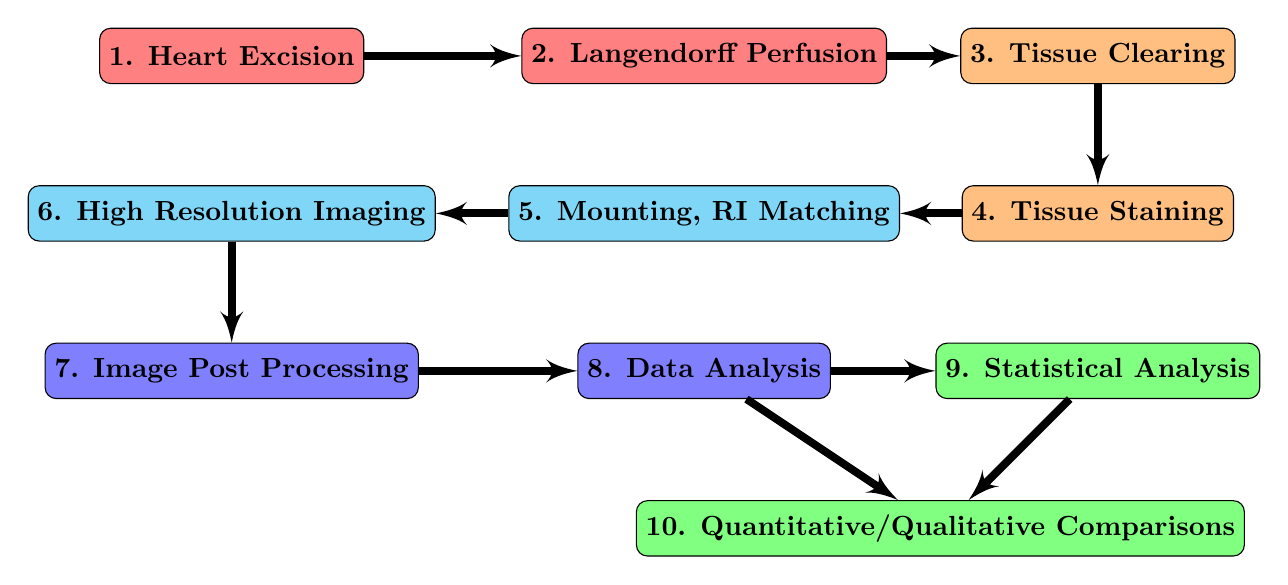
\begin{tikzpicture}
        \tikzstyle{terminator} = [rectangle, draw, text centered, rounded corners, minimum height=2em]
        \tikzstyle{connector} = [draw, -latex',line width=1mm]
        \node [terminator, fill=red!50] at (-6,-1) (start) {\textbf{1. Heart Excision}};
        \node [terminator, fill=red!50] at (0,-1) (one) {\textbf{2. Langendorff Perfusion}};
        \node [terminator, fill=orange!50] at (5,-1) (two) {\textbf{3. Tissue Clearing}};
        \node [terminator, fill=orange!50] at (5,-3) (three) {\textbf{4. Tissue Staining}};
        \node [terminator, fill=cyan!50] at (0,-3) (four) {\textbf{5. Mounting, RI Matching}};
        \node [terminator, fill=cyan!50] at (-6,-3) (five) {\textbf{6. High Resolution Imaging}};
        \node [terminator, fill=blue!50] at (-6,-5) (six) {\textbf{7. Image Post Processing}};
        \node [terminator, fill=blue!50] at (0,-5) (seven) {\textbf{8. Data Analysis}};
        \node [terminator, fill=green!50] at (5,-5) (eight) {\textbf{9. Statistical Analysis}};
        \node [terminator, fill=green!50] at (3,-7) (nine) {\textbf{10. Quantitative/Qualitative Comparisons}};
       
        \path [connector] (start) -- (one);
        \path [connector] (one) -- (two);
        \path [connector] (two) -- (three);
        \path [connector] (three) -- (four);
        \path [connector] (four) -- (five);
        \path [connector] (five) -- (six);
        \path [connector] (six) -- (seven);
        \path [connector] (seven) -- (eight);
        \path [connector] (seven) -- (nine);
        \path [connector] (eight) -- (nine);
    
    \end{tikzpicture}
    
    \caption{\textbf{Overview flowchart of optimized pipeline for imaging of cleared cardiac tissue.} Each section of the pipeline utilizes protocols originating from independent fields of research applied here for use in acquiring structural images of cardiac tissue: cardiovascular science protocols (Red, 1-2), biochemical protocols (Orange, 3-4), optical physics protocols (Cyan, 5-6), computer science protocols (Purple, 7-8), mathematics/statistical protocols (Green, 9-10).}
    \label{fig:enter-label}
\end{figure}

The focus of the thesis is thus the development and successful application of the tissue imaging pipeline for use in structural analysis of cardiac tissue samples for use in cardiovascular research. To accomplish this goal, key aspects of the pipeline must be optimized and characterised to ensure pipeline steps originating from different fields of research and development remains compatible for use in sequence and does not inhibit the capability of the pipeline to produce images of high resolution and fidelity for use in qualitative and quantitative histological analysis such as measurements of signal intensity, cellular density, or structural dimensions.

Figure 1.1 diagrams the ten key steps of the assembled pipeline created from start to end. Interdisciplinary contributions to the pipeline from the research fields of cardiovascular science, biochemistry, optical physics, computer science are also identified in the figure, demonstrating the vital role cross discipline collaboration played in the assembly of the pipeline. Chapter 2 and 3 will detail protocols in the pipeline already established and commercially available in the fields of cardiovascular science, physics, computer science, and chemistry. These protocols were adopted for use in the imaging pipeline with minor modifications made by myself alongside research collaborators to better accommodate their application to cardiac tissue samples. In addition, chapter 3 will focus on characterization tests performed on cleared tissue samples to confirm the preservation of tissue structure upon the completion of the clearing protocols. Chapter 4 presents protocols original to this project: tissue mounting and image processing procedures. These processes were created and characterized specifically for use in the imaging pipeline. Finally, in chapter 7, the completed imaging pipeline is applied to three ongoing research projects being conducted by research collaborators to demonstrate the versatility of the pipeline for use in experimental and research settings.

It is clear that the created imaging pipeline has implemented protocols and concepts from a wide span of scientifics disciplines to achieve the goal of acquiring three dimensional structural images of cardiac tissue. As such the remainder of this chapter is set up to provide the contextual background across each of these associated fields: biology, chemistry, engineering, and optical physics whose protocols were thereafter applied throughout the course of this project.

\section{Cardiac Physiology}
\subsection{Cardiac Structure}
The human heart is the key component of the human circulatory system which pumps blood across the entire body to ensure the perpetual transfer of oxygen and nutrients into cells and the expulsion of carbon dioxide and waste materials out \cite{saltzman_biomedical_2015}. This pump function of the heart is measured in medicine as the ejection fraction, the fraction of blood inside the heart that the heart can pump out in a single heartbeat \cite{golla_heart_2025} When a heart is operating under normal conditions in humans, ejection fractions are seen to be at 50\% or higher \cite{golla_heart_2025}. 

To achieve this level of pumping efficiency, the cells that compose the majority heart tissue, cardiomyocytes (CMs), are highly specialized to prioritise the perpetual and rhythmic sequences of movement that continues the pumping of blood \cite{woodcock_cardiomyocytes_2005}. A diagram showcasing the structure of the heart organ and organization of CMs within the organ is shown in Figure 1.1.

\begin{figure}[H]
    \centering
    \includegraphics[width=0.85\linewidth]{Figures/Figure1.1.png}
    \caption{\textbf{Diagram of cardiac and cardiomyocyte structure and features}. Main figure details overall organ structure. Middle inset: structure of Left Ventricle (LV) wall in the organ, Left inset: structure of myocardium region in the LV wall. Created in  https://BioRender.com.}
    \label{fig:enter-label}
\end{figure}

Some of the key features that distinguish CMs from all other cell and muscle types in the body include: high concentrations of mitochondria (5,000-8,000 per cell), striated and branching cell shapes, connection to other CMs via intercalated discs and gap junctions []. These features, in combination with the use of ion channels and protein pumps in the cardiomyocyte membrane, enable cardiac tissue to maintain the high metabolic activity required for high speed, synchronized contraction without fatiguing \cite{woodcock_cardiomyocytes_2005}. 



\subsection{Cardiac Electrophysiology}
To perform this rhythmic contraction and relaxation of CMs in the heart, a sequence of electrical signals is transmitted to and throughout the organ via a network of nerve cells \cite{saltzman_biomedical_2015}. A diagram showing the path, key structures, and pattern of electrical depolarization across the heart to form the heart beat is shown in Figure \ref{fig:HeartElec}:

\begin{figure}[H]
    \centering
    \includegraphics[width=0.85\linewidth]{Figures/Figure1.2.png}
    \caption{\textbf{Diagram of the heart and key structures for cardiac electrical activity.} Red arrows indicate direction of depolarization from SA Node to Perkinje Fibre network throughout the heart. Created in  https://BioRender.com. }
    \label{fig:HeartElec}
\end{figure}

Initiating signals generated by the sympathetic and parasympathetic nervous system is introduced to the organ at the Sinoatrial (SA) Node located in the right atrium chamber of the heart. The cells of the SA Node rhythmically depolarize in response to these signals originating from the brain[]. The depolarizing sequences then traverse the tissue of the right atrium via a series of internodal tracts to the Atrioventricular (AV) Node and the Bundle of His located near the centre of the heart. At the Bundle of His, depolarization progresses on to the upper corners of the ventricles closest to the bundle before then traversing down bundle branches and across the rest of the ventricular myocardium. The wave of depolarization across the myocardium concludes at the Perkinje fibre network at the end of the branch network \cite{saltzman_biomedical_2015}. All remaining cardiac tissue has depolarized by this point, which is followed immediately by repolarization of the myocardium in preparation for the next wave of depolarization \cite{saltzman_biomedical_2015}.

\subsection{Myocardial Infarction Alterations}

The need for rapid and perpetual repolarizing of cells in the myocardium requires massive investment of the CM metabolic activity and time. The consequence of devoting so much cell function to this feature is the cessation of other cellular activities commonly seen in eukaryotic cells. This includes the ability for these cells to replicate and repopulate by means of mitosis, which is possible to some extent in most other tissues in the human body. Skeletal muscles, red blood cells, and neurons are also incapable of replication, but all have alternative means of replacing lost or damaged cells such as the use of myosatellite cells in skeletal muscles, neuroplasticity in neurons, and red blood cell formation in bone marrow \cite{paxton_leeds_2003}. No such alternative exists for terminally differentiated CMs after the population of differentiable stem cells is depleted in early stages of human development \cite{uygur_mechanisms_2016}. 

 The process of tissue remodelling in the heart tissue is the result of myocardial infarctions (MIs). A MI is instigated in by a loss of blood flow to a region of the heart due, in most cases, to obstructions in the coronary vessels delivering oxygenated and nutrient rich blood to the myocardium. With no means of replacing or repairing lost or damaged tissue, the immune system of the body defaults instead to a process of cardiac remodelling to prevent the heart from bursting through the damaged region at the heart continues to pump blood \cite{huethorst_development_2022}.  Once the remodelling is complete, three unique regions in the cellular matrix of the heart muscle emerge \cite{huethorst_development_2022}. These regions, and features unique to each, are shown in Figure \ref{fig:postMI}. 

\begin{figure}[H]
    \centering
    \includegraphics[width=0.85\linewidth]{Figures/Figure1.3.png}
    \caption{\textbf{Diagram of heart tissue regions post-MI.} Close up inset legend: (A) MI heart healthy zone, (B) MI heart border zone, (C) MI heart scar zone. Created in  https://BioRender.com.}
    \label{fig:postMI}
\end{figure}

In the post-MI heart, healthy zones (Figure 1.3, Inset (A)) are the remaining regions of cardiac tissue that remain active and operation post-MI with the ability to contact and propagate electrical activity as normal. Conversely, Scar Zones (Figure 1.3, Inset (C)) are those regions of tissue where the CMs have died, being replaced with fibrotic scar tissue. This scar tissue has no ability to contract or propagate electrical activity. In between these two regions is the Border Zone (Figure 1.3, Inset (B)) which are regions that possess a mixture of active and deceased cells in varying ratios which still has limited, sporadic ability to contact and propagate electrical signals \cite{huethorst_development_2022}.

With their high metabolic demands, CMs undergo uncontrolled cell death, necrosis, quickly after being cut from their continuous supply of oxygen and nutrients \cite{huethorst_development_2022}. With each cardiomyocyte lost, the collective strength of the cardiac tissue degrades and the electrical activity that perpetuates rhythmic heart beating is interrupted as the dead cellular tissue is no longer able to perpetuate the waves of electrical depolarization to adjacent cells awaiting the signal to propagate the heart’s pumping activity. Should a sufficiently high number of CMs undergo necrosis, the ejection fraction of the heart will reduce to less than 40\% of the total blood in the heart, leading to heart failure. This failure is fatal without immediate medical treatment to restore or substitute cardiac activity and resume the flow of nutrient rich blood through the body \cite{golla_heart_2025}. 

The emergence of scar and border zones in the myocardium can also gradually introduce disturbances in heart rhythm, known as arrhythmias, that can increase in severity over time. The increase in severity stems from the scar region gradually stiffening over time, restraining movement of surrounding healthy tissue. The unregulated proliferation of nerve cells in border zones also gradually introduces disturbances in heart rhythms, leading to irregular patterns of depolarization to the surrounding healthy tissue that contribute to arrhythmia formation \cite{amoni_heterogeneity_2023, huethorst_development_2022}. Severe arrhythmias can eventually result in cardiac arrest should the irregular beat becomes too unstable and thus inefficient to pump sufficient blood throughout the body. This condition is highly lethal if not immediately treated and remains one of the leading causes of death for those living with hearts altered by MIs \cite{golla_heart_2025}.  




\section{Light Sheet Fluorescence Microscopy}
% REFERCES GIARDINI, OLIANTI THESES, mesoSPIM Paper

\subsection{Conceptual Premise}
To examine three dimensional structural changes in infracted hearts compared to healthy hearts, the imaging technique utilized must be capable of recording images of large volumes of tissue in reasonable amounts of time and with high, consistent spatial resolution. This leads to the selection Light Sheet Fluorescence Microscopy (LSFM) as the optical imaging technique of choice for this application.  

The main principle behind LSFM is the idea of using perpendicular pathways in excitation and detection to permit the simultaneous illumination and observation of a narrow plane of space across the system’s field of view \cite{voigt_mesospim_2019}. The excitation path consists of a Gaussian beam that uses galvanometer mirrors to shift the beam laterally to form the light sheet of the system. The basic setup of this method and a detailed look of the Gaussian beam and associated dimensions are shown in Figure 1.4.

\begin{figure}[H]
    \centering
    \includegraphics[width=0.75\linewidth]{Figures/Figure1.4.png}
    \caption{\textbf{Optical Diagram and Associated Components of Light Sheet Fluorescence Microscopy (LSFM).}}
    \label{fig:enter-label}
\end{figure}

When fluorescently stained samples traverse the plane of the light sheet, that plane of tissue will be illuminated and can be viewed by the scientific camera with high contrast, while the remainder of the sample remains unilluminated and not visible. The sample can then be shifted through the light sheet with the camera capturing images of each plane of the sample, recording the entire volume into a single image stack for use in analysis.

In theory, this microscopy concept can generate multiple thin slices images of a sample with high resolution and optical sectioning. LSFM is also capable of recording this data in relatively short periods of time as the separation of the excitation and emission pathways allows signal across the entire FOV to be recorded simultaneously rather than in sections \cite{poola_light_2019}. These image collections can then be recombined digitally to obtain a full three-dimensional image of the sample recorded. The ability to image across the volume without the need for excision or slicing has the added benefit of preserving any structural features that would otherwise be lost in the process of sectioning the tissue to conform to more standardized methods of microscopy.

An additional benefit to this microscopy method is the reduction of photobleaching and phototoxicity that can occur in tissue samples due to overexposure to high powered sources of illumination. By expanding the illumination from a singular point to across an entire plane of the imaging, the intensity of the emitted light is diluted, allowing for longer imaging sessions to occur more frequently with reduced risk of damage to the tissue or loss of fluorescence after repeated. excitation.

\subsection{Axially Scanned Light Sheet}
The use of a light sheet to illuminate a thin plane across the field of view can also have the added benefit of being capable of generating homogenous resolution images across large fields of view. This can be achieved through the technique called Axial Scanning Light-sheet Microscopy (ASLM). This technique takes advantage of the unique characteristics of the Gaussian Beam, which is detailed in Figure \ref{gb}.

\begin{figure}[H]
    \centering
    \includegraphics[width=0.85\linewidth]{Figures/GaussianProfileDiagram.png}
    \caption{\textbf{LSFM Gaussian Beam Profile.} Legend: \(w_0\)= Beam Waist, \(Z_R\) = Rayleigh Length, b = Depth of Focus, w(z)= Gaussian Beam Width, \(\theta \) = Total Angular Spread. Beam region within depth of focus range highlighted in cyan. Insets (B),(C) showcase relation between $w_0$ and b.\cite{paschotta_gaussian_2005}}
    \label{fig:gb}\
\end{figure}

The thickness of the Gaussian beam follows a well established characterization formula: 

\begin{equation}
w(z) = w_0 \sqrt((1+(\frac{z}{z_R})^2)
\end{equation}
\medskip

The minimum thickness of the Gaussian beam is located at the beam waist ($w_0$) and its relation to the light wavelength and the Numerical Aperture (NA) of the Excitation pathway is given by:

\begin{equation}
w_0 = \frac{\lambda}{NA*\pi}
\end{equation}
\medskip

Similarly, the Depth of Focus (b) spans across the beam and defines the region where the the bean thickness (w(z)) is similar enough in value to the beam waist to be considered consistently concentrated for use in acquiring homogenously resolved images \cite{paschotta_gaussian_2005}. The depth of focus relation to the beam waist is given by:

\begin{equation}
b = \frac{2\pi w_0^2}{\lambda}
\end{equation}
\medskip

Due to these interconnected relations between the NA, depth of focus, and beam waist, it is possible to expand or reduce the dimensions of the beam by adjusting the NA of the excitation pathway. As shown in insets (B,C) of \ref{gb}: decreasing the NA of the system, the depth of focus will increase but at the cost of increasing the beam waist, lowering the resolution the beam can resolve the process. Conversely: by increasing the NA, the beam waist can be reduced to record at higher resolutions but at the cost of shortening the depths of focus. While the LSFM system will be able to record at higher resolution with a high excitation NA, it will only be able to do so in the central region of the camera FOV as the depth of focus will no longer span the length of the FOV. This leaves the left and right sides of frames recorded at a low resolution compared to the middle. ASLM resolves this issue to generate homogenously resolved images by utilizing tuneable lenses and camera rolling shutters as diagrammed in Figure \ref{aslm}. 

\begin{figure}[H]
    \centering
    \includegraphics[width=0.85\linewidth]{Figures/ASLMDiagram.png}
    \caption{\textbf{Diagram of ASLM Imaging Technique.} Comparison of Traditional (left) and Axial Scanned (right) Light Sheet Image Acquisition. Region of Light Sheet Within Depth of Focus (b) Labelled, Shown In Green}
    \label{fig:aslm}\
\end{figure}

By synchronizing the camera rolling shutter to the shifting of the beam waist across the frame, the scientific camera will record the narrow spans of pixels in the frame where the beam waist is located as it shifts locations \cite{voigt_mesospim_2019}. The camera will then digitally combine all of these narrow spans together into a complete frame covering the entire FOV, forming an image in which the beam waist is present across the entire image and therefore is homogeneously resolved. 

\subsection{Practical Limitations}

Light Sheet Microscopy techniques, of both traditional and axial scanned variations, have two obvious limitation which impairs the usability of this method for volumetric imaging of tissue samples: 

\begin{enumerate}
    \item Vast majority of LSFM systems in use today are incapable of accommodating thicker, non sectioned samples \cite{poola_light_2019}.
    \item Tissues found in biology are insufficiently transparent to allow optical sectioning to occur \cite{olianti_optical_2021}.
\end{enumerate}

\subsubsection{Tissue Volume in LSFM Systems}
Most LSFM systems developed and made commercially available are unable to accommodate larger volume samples that are not physically sectioned into micron thick slices. This is due to the complicated hardware and optical pathways surrounding the sample making manipulation of samples across light sheets for distances greater a few millimetres extremely difficult \cite{krzic_multiview_2012, poola_light_2019, gualda_openspinmicroscopy_2013}. To compound the problem, due to the relation between the Gaussian beam waist and the depth of focus, to obtain the highest resolutions possible, the usable region of the light sheet will be incredibly narrow even with the application of ASLM into the system. This will result in the need for image tiles numbering in the hundreds of tiles to cover samples with large surface areas, making complete reconstruction of tissue volumes extremely time consuming and computer process intensive to complete \cite{poola_light_2019}.

\subsubsection{Tissue Transparency in LSFM Systems}
 The second issue encountered when attempting to image mesoscale samples comes from the opacity of the tissues themselves. Even if the Gaussian beam is sufficiently powerful for the light sheet to successfully penetrate across the tissue, any fluorescent emission created as a result will not be intense enough to exit back out of the tissue towards the detection objective and camera. There is also the possibility for such high power light to cause damage to the tissue and quench the fluorescence of dyes in the sample, rendering the tissue incapable of producing images of any degree of quality regardless of the tissue's opacity.

This opacity stems from the refractive index (RI) mismatch between the various biomolecules inside the tissue (lipids, proteins, blood, water, et cetera) and the surrounding external environment (atmospheric air) \cite{paysan_art_2023}. This optical metric quantifies the reduction in speed experienced by incident light when propagated through a given medium. Sudden changes in RI that can occur as light travels across two mediums can severely hinder the propagation of light, leading to an increase in light scattering and in turn increase the opacity of the medium the light enters.

The sudden and drastic change in RI between air (RI $\approx$ 1.0) and cardiac tissue ( RI $\approx$ 1.382) will scatter the light upon contact to the tissue surface, preventing the Gaussian beam from forming the desired beam waist. Traditionally, in biological histology, the solution to this issue would be to physically slice samples into extremely thin slices, defeating the purpose of using the LSFM technique for volumetric imaging. To solve this issue without sectioning the tissue, several LSFM systems have implemented engineered excitation beams such as Bessel, airy, and lattice beams to reduce scattering and improve penetration into the tissue volume without light diffraction \cite{sapoznik_single-objective_2020, poola_light_2019}. This method of tissue clearing is the preferred methods to overcoming this obstacle with respect to large volume imaging as the use of engineered beams in LSFM requires mechanically complex and costly setups which limit the viability of wide scale use in research. As a result, instead of changing the beam utilized, the preferred method of choice to overcome this obstacle is to change the tissue itself via chemical treatments to increase the transparency of the tissue. This form of chemical treatment, known as tissue clearing, allows the Gaussian beam to traverse the sample with lower light scattering and absorption. 


\section{Tissue Clearing Protocols}
\subsection{Conceptual Premise}
Chemical treatment of biological tissues to render them translucent or even fully transparent has been a field of research explored by researchers for well over a century \cite{paysan_art_2023}. The technique of tissue clearing aims to homogenize the RI of tissues composed of heterogenously organized biomolecules. The biomolecules most influential to the RI mismatch of tissues to its ex situ environment include water (RI = 1.33), lipids ($RI \approx 1.44$), and proteins ($RI \approx 1.43$). To achieve closer (if not near perfect) RI homogeneity, clearing processes seek to remove, alter, and/or replace one or more of these biomolecules from the tissue without altering the existing internal structure. This will allow the remaining molecules of similar RI to be matched to the RI of the external environment via immersion into a solution with an equal RI value \cite{paysan_art_2023, tainaka_chemical_2018}. Fully immersed, the entire sample volume will now be fully RI matched and can hereafter be imaged with LSFM, taking advantage of the techniques optical sectioning with no further hindrance. An example of how effective tissue clearing can be in rendering tissues optically transparent, a before and after comparison photo showcasing a tissue before clearing, after clearing, and after immersion in RI matched solution is shown in the following Figure:

\begin{figure}[H]
    \centering
    \includegraphics[width=0.85\linewidth]{Figures/Figure1.7.png}
    \caption{\textbf{Tissue Transparency Before and After Tissue Clearing.} 400 micron thick Leporine tissue slice before clearing (A), after clearing (B), and after RI matched solution immersion (C). Sample processed using CLARITY method of tissue clearing (see section 3.2 of this chapter).}
    \label{fig:enter-label}\
\end{figure}

\subsection{Methodology Variations}


Three categories of clearing methodologies have emerged which utilize unique chemical processes to achieve RI matching of tissue to their \textit{ex vivo} environment. Each of these categories (dehydrating, hyper-hydrating, and hydrogel-hybridizing) have unique advantages and disadvantages to each in addition to containing a wide variety of sub-categories and variations that fall under the umbrella of each category \cite{paysan_art_2023}. This wide range of clearing options is also perpetually expanding in size as new methods and variants are published in this field on a regular basis. 

\subsubsection{\textit{Dehydration Methods}}
Dehydration methods of tissue clearing utilizes alcohol solution immersion to dehydrate the tissue, raising the RI as water is expelled along with dissolved lipids \cite{paysan_art_2023}. Samples thereafter are immersed in an organic solvent with an RI matching that of proteins in the tissue. This solvent removes any remaining lipids as it intercalates with the cellular structures inside the tissue. With the solvent now replacing the water and lipids in the tissue structure, the RI has been homogenized to the solvent and rendered transparent. 

While simplistic and fast to perform to completion, the dehydration method causes considerable alteration to tissue structure \textit{ex vivo} \cite{olianti_optical_2021}. This makes analysis of the cleared tissue structure unviable for biological analysis as the structure should be preserved as close as possible to \textit{in vivo} conditions. Doing so will allow for the most accurate insight into the biological activity of interest to be obtained.

\subsubsection{\textit{Hyper-hydrating Methods}}
Methods of the hyper-hydrating (or hydrophilic in some publications) variety utilize non-hydrophobic detergent solutions to extract lipids from the sample. This occurs as a result of an osmotic gradient that forms inside the tissue cellular structures, allowing water to penetrate into regions of the cells it would not normally be able to reach \cite{paysan_art_2023}. As lipids gradually diffuse out of the tissue, the structure remains mostly intact (depending on the detergents used) and expands in volume with the retention of additional water. This expansion is mitigated once the sample is removed from the detergent and placed in a RI matching solution (RIMS), expelling the water, being replaced with the intercalating solution that homogenizes the remaining tissue to its RI.

Hyper-hydrating methods of clearing can vary wildly in quality and in their ability to preserve tissue structure. Numerous combinations of detergents, alcohols, and solvents have been tested with certain combinations performing well with certain tissue types and poorly in others \cite{paysan_art_2023, olianti_optical_2021, susaki_whole-brain_2014}. Careful consideration is therefore required in selecting a specific method in this category, with through testing performed beforehand to confirm the viability of a method for use in clearing a specific tissue type with minimal alteration to in situ structure. 

\paragraph{CUBIC: Cleared Unobstructed Body Imaging Cocktails}
Of the hyper-hydrating methods of tissue clearing, the CUBIC family of clearing protocols provide some of the best clearing results among hyper-hydrating methods with minimal alteration to tissue structure after completion of the process \cite{susaki_whole-brain_2014, tainaka_chemical_2018}. Several variations of of the CUBIC protocol have been developed and made commercially available since the initial publication in 2014 by the CUBIC Stars team at the University of Tokyo. These cocktail varieties allow the protocol to be used with a variety or combination of tissue types up to and including entire animal bodies \cite{noauthor_cubic_nodate}. The CUBIC second generation variant, CUBIC-L/RA, is one such protocol that has been shown in previous publications by the developers and independent researchers to have the best capability among the CUBIC family of chemical cocktails to clear cardiomyocyte samples with minimal structural change and preservation of dye fluorescence after immersion in RIMS \cite{tainaka_chemical_2018}. As such, this makes CUBIC-L/RA the most optimal choices on the market today for cardiomyocyte clearing by hyper-hydrating means. 

\subsubsection{\textit{Hydrogel-Hybridizing Methods}}
Developments in past decade has led to the rise in the use and efficiency of methods which remove entire categories of molecules from tissue samples. In their place, these methods create hydrogel matrices that maintain the structure of the sample without the RI mismatch of the original molecules \cite{paysan_art_2023}. This is achieved by exposing tissue samples to monomers and a fixative chemical which induces a polymerized hydrogel mesh to be formed across the tissue volume. The matrix serves a scaffold holding proteins and other molecules of interest in position while allowing unwanted molecules causing RI mismatch, such as lipids, to be removed from the tissue using highly concentrated detergent solutions. Immersion in RIMS will complete the clearing process with the hydrogel-hybridized tissue quickly homogenizing to the solution. Hydrogel-Hybridized methods are capable of rendering tissue transparent to the point of becoming invisible to the human eye when immersed in RIMS. As such, techniques based in this method are well regarded in the research field as producing the highest quality tissue clearing achievable today. 

One major issue present in many hydrogel-hybridizing methods is that they tend to decrease the structural stability of the tissue as the hydrogel matrix which preserves the tissue structure is itself highly gelatinous. Cleared samples can be damaged easily when handling of the sample. As the sample acquires a slippery, gelatinous condition after clearing, the additional fragility makes handling of these tissue extremely difficult and time consuming. Further complicating adoption of these methods for use in research is the fact that the processes of polymerizing the acrylamide polymer and removing lipids from the tissue can be very complex and time consuming to properly complete. Specialized equipment including (but not limited to) pressurized gas, vacuum chambers, fume hoods, and safety gear can be required to properly polymerize the monomer \cite{olianti_optical_2021}. Detergent clearing, while simpler to perform compared to polymerization, can require several weeks to months to complete depending on the tissue type and volume .

\paragraph{CLARITY: Clear Lipid-exchanged Acrylamide-hybridized Rigid Imaging Tissue Hydrogel}

The most prominent hydrogel-hybridizing methods of tissue clearing is the CLARITY method, which utilizes a combination of acrylamide and bis-acrylamide monomers to form the hydrogel mesh via polymerization in Nitrogen gas . The lipids of the sample can then be removed by immersion in a solution of Sodium Doedecyl-Sulfate (SDS) over the course of 4 to 6 months\cite{olianti_optical_2021}. The cleared tissue could then be RI matched using a proprietary RIMS solution designed specifically to match with the RI of CLARITY cleared samples.  While the process is extremely time consuming and complex to perform, previous results achieved using the method with cardiomyocyte samples still makes the CLARITY methods one of most effective clearing protocols for cardiac tissue clearing in use today \cite{paysan_art_2023,olianti_optical_2021}. 

\section{Chapter Summary}

This chapter has set out to present the primary aim of this project: the development and successful application of a novel tissue imaging pipeline for use in structural analysis of cardiac tissue samples for use in cardiovascular research. The unique features and characteristics of cardiac tissue have been detailed here, explaining the processes by which structural modification as a result of MIs occur and proceed to degrade cardiac function over time. The importance of better understanding how these alterations occurred in the 3D structure of the myocardium is made evident and the means by which this information can be acquired is detailed in sections 1.2-3. Light Sheet Fluorescence Microscopy, in combination with Tissue Clearing Techniques, provides a basis by which the 3D volumetric imaging of cardiac tissue samples can be accomplished. To do this, an appropriate LSFM system, which is capable of overcoming limitations previously described in most LSFM systems, must be selected, assembled, and optimized for use in this newly formed imaging pipeline. This is the focus of the next chapter, which will also detail the acquisition, processing, storage of data recorded from the microscope into the PC for use in subsequent image analysis. 



\chapter{The mesoSPIM Microscope}

The aim of this chapter is to introduce the mesoSPIM microscope and its associated protocols utilized to record and process structural, volumetric images of cardiac tissue. The design and operation of the mesoSPIM system essential to achieve peak performance in the imaging pipeline are explained here in detail along with those imaging protocols implemented with the system's control software. Further to this, in this chapter, data processing and storage protocols were implemented. These protocols demonstrate an efficient and reliable means by which the multiple terabytes of data recorded by the mesoSPIM hardware can be managed. When combined, these mesoSPIM hardware and software based protocols provide the high imaging throughput and quality essential for the success of the imaging pipeline to achieve its intended goals.

\section{mesoSPIM Microscope}

This open source LSFM system was selected for its well documented ability to image mesoscale samples (up to 90 $cm^3$) of tissue by physically rotating and shifting the sample across and through the formed light sheet utilizing low NA excitation objectives and ASLM to generate isotropic, high resolution images over a large camera FOV (~216 $mm^2$) \cite{voigt_mesospim_2019}. This is in stark contrast to other commercially available and open source LSFM systems, which are unable to physically move the sample or are only able to shift the light sheet a few hundred micron across the sample \cite{poola_light_2019}. Many of these systems are also unable to capture FOVs greater than 16 $mm^2$, increasing the amount of post-processing required to stitch together images to reassemble tissue volumes \cite{poola_light_2019}. It is because of these features and the open source design of the system allowing for customizations to the system function and design to be easily implemented compared to commercially sold systems that the mesoSPIM was selected as the LSFM of choice for use in the cardiac tissue imaging pipeline developed in this project. 

\subsection{System Overview}
The upgraded version 5 mesoscale Selective Plane Illumination Microscopy (mesoSPIM) system was constructed in accordance with the publication and open-source documentation provided by the mesoSPIM Initiative \cite{voigt_mesospim_2019,vladimirov_benchtop_2024}. Custom components and components requiring modification were fabricated utilizing 3D printers as well as industrial workshop services made available by the University of Glasgow’s School of Physics and Astronomy. Full assembly documentation (including components lists, photos, manufacturer details, schematics, figures, and references) can be found on the mesoSPIM Initiative Website and GitHub account \cite{vladimirov_mesospimbenchtop-hardware_2025}.

\begin{figure}[H]
    \centering
    \begin{subfigure}[a]{0.75\textwidth}
    \centering
    \includegraphics[width=1\linewidth]{Images/OverviewPhoto.jpg}
    \caption{Overview photo.}
    \end{subfigure}
    \medskip
   
    \begin{subfigure}[b]{0.75\textwidth}
    \centering
    \includegraphics[width=1\linewidth]{Figures/Overview Diagram.png}
    \caption{Overview diagram. Isometric view from right side of system. Main components and location in overall setup highlighted. Additional structural supports, left side excitation arm, power/signal electrical wiring, and external dark box are not included in diagram for ease of viewing. (Diagram Not To Scale)}
    \end{subfigure}
   
   
    \caption{\textbf{Overview photo (a) and diagram (b) of the fully assembled, upgraded ver.5 mesoSPIM used in the imaging pipeline developed.}}
\end{figure}

The mesoSPIM microscopy system consists of three main components connected to a central PC that operates and synchronizes movement to permit light sheet imaging across mesoscale volumes with homogeneous, isotropic resolution in the range of 8-12 microns in the axial and lateral directions (See chapter 1, section 2.1 for LSM conceptual details). These three components includes the detection pathway, the single side excitation pathways, and the sample gantry. The following table details the resolutions achieved using this system in axial and lateral resolution as reported by the original system developers along with those resolution limits recorded  using the two unique imaging modalities performed with the system used during the course of this project.


\begin{table}[H]
            \begin{tabular}{|c|c|c|c|}
        \medskip
         \textbf{Modality} &\textbf{ Lateral (X)} & \textbf{Lateral (Y)} & \textbf{Axial (Z)}\\\hline
         
         mesoSPIM Initiative Protocol \cite{voigt_mesospim_2019} & $1.5 \mu m $ &$1.5 \mu m$  & $3.3 \mu m$ \\
         
         Mounted Sliced Tissue Protocol & $4.66\pm0.67\mu m$ & $3.86\pm0.49\mu m$ & $7.76\pm1.64\mu m$\\
        
         Mounted Left Ventricle Section Protocol & $4.19\pm0.64\mu m $& 3.85$\pm0.42\mu m$ & 4.61$\pm1.12\mu m$\\\hline
         
    \end{tabular}
    \medskip
    \caption{\textbf{Resolution limits of upgraded Version 5 mesoSPIM microscope assembly utilizing established and experimental imaging modalities.} Details regarding mounted sample imaging protocols provided in Chapter 2, Section 3. Acquisition of resolution limits detailed in chapter 4, section 2.}
\end{table}

 


\subsection{Single Sided Excitation Pathway}
The first component of the mesoSPIM system are the excitation pathways located on elevated platforms to the immediate left and right of the detection pathway’s objectives. These pathways connect to the laser engine to the shutters, electronically tuneable lenses, and galvanometer mirrors that performs the ASLM imaging technique utilized by the mesoSPIM for imaging large tissue volumes (See Chapter 1, Section 2.2 for ASLM conceptual details). An image and optical pathway diagram of the fully assembled and aligned right side excitation pathway is seen in Figure 2.2(a) and (b).

\begin{figure}[H]
    \centering
    \begin{subfigure}[a]{0.75\textwidth}
    \centering
    \includegraphics[width=1\linewidth]{Images/ExcitationPathPhoto.jpg}
    \caption{Photo of excitation pathway on right side of mesoSPIM.}
    \end{subfigure}
    \medskip
    
    \begin{subfigure}[b]{0.75\textwidth}
    \centering
    \includegraphics[width=1\linewidth]{Figures/Excitation Diagram.png}
    \caption{Excitation laser 2D and 3D (insert) optical pathway diagrams (Diagram not to scale). Legend - ETL: electronically tunable lens; M1-3: mirrors; L1-2: lenses; GM: galvanometer mirror; SL: scan lens; SC: sample chamber. Left side excitation arm is YZ plane mirrored duplicate of right side arm.}
    \end{subfigure}
    \caption{\textbf{Fully assembled upgraded ver.5 mesoSPIM excitation pathway image (a) and diagrams (b)}}
    \label{fig:enter-label}
\end{figure}

A multiple channel laser engine (Omicron-Laserage GmbH, LightHUB ULTRA) was installed to generate the excitation beams used in the formation of the Gaussian beam. This engine allows for the installation of multiple laser lines with a custom selection of power levels and wavelengths which can be installed and uninstalled at anytime by me without the need to send the device back to the manufacturer. The laser lines can be  activated and deactivated seamlessly through the engines proprietary software as well as the mesoSPIM General User Interface (GUI). A table listing the laser lines installed in the laser engine for the purposes of research conducted in this project is shown in Figure 2.3: 


\begin{table} [ht]
    \centering
    
    \begin{tabular}{cccc}
            \medskip
            \textbf{Laser Line} & \textbf{Wavelength} & \textbf{Documented Max Power}\\ \hline
             \medskip
            LuxX CW Diode Laser 647& 647nm & 140mW\\
             \medskip
            OBIS LS Laser 532 & 532nm & 120mW\\
             \medskip
            LuxX CW Diode Laser 488 & 488nm & 100mW\\
             \medskip
            LuxX CW Diode Laser 405&  405nm & 120mW\\ \hline
             \medskip
    \end{tabular}
    \caption{\textbf{Laser lines installed into LightHUB Ultra\textsuperscript{\textregistered} Laser Engine}}
    \label{tab:my_label}
\end{table}

Following from the emission of the laser beam in the laser engine, the beam proceeds to pass through a beam expander followed by Electronically Tuneable Lenses (Optotune, EL-16-40-TC-VIS-5D-1-C) installed into each excitation arm. These ETLs allow the narrowest region of the Gaussian beam to shift (in x-axis) across the imaging field of view, as is required for axial scanning to occur. Continuing from the ETL aperture, the beam is reflected off of galvo scanning mirror (Thorlabs GVS211) directly into the back focal plane of modified Nikon camera lenses (AF-S 50mm f/1.4G). These lenses have had their internal apertures set to fully open, allowing them to acts as an f-theta configured objective lenses. The galvo scanning mirror allows the 10 mm diameter beam (Numerical Aperture, NA = 0.1) to shift back and forth in the y-axis to form the light sheet inside the sample chamber that can provide homogeneous illumination for sample imaging.

Assembly of the excitation arm structural supports, electrical wiring, and elevated platforms were completed by myself. Delicate modifications to Nikon scan lenses required for installation into the excitation. This included the removal of sections of the external lens frame as well as the locking the internal aperture of the lens into the fully open position. Caution was taken during these steps to not scratch or damage the lens as these alterations were made. Installation and Alignment of the optical components of the excitation arms were completed by Dr. Sharika Mohanan in accordance with alignment protocols provided by the mesoSPIM Initiative \cite{vladimirov_mesospimbenchtop-hardware_2025}. 

For the purposes of our research, all imaging was completed using only the excitation pathway on the right side of the detection pathway. This was done to allow full laser engine power (100mW to 140mW) to be dedicated to a single excitation path instead of utilizing a beam splitter to split the emitted laser across both pathways, cutting the maximum excitation laser power achievable by the system in half in the process (50mW to 70mW). Though inactive, the right side excitation arm was kept intact for use in imaging should the left side arm at any point encounter technical or optical issues. Beam splitter, fibre switch, and other components required to permit dual side illumination were also kept installed into the system or stored nearby for potential future use should higher power laser lines be installed into the laser engine.

\newpage

\subsection{Detection Pathway}
The detection pathway consists of (following the direction of emitted light travel): the microscope objective, emission filter wheel, tube lens, and finally an sCMOS camera. An image and diagram of the fully assembled detection pathway are shown in Figure 2.3(a) and (b) respectively.

\begin{figure}[H]
    \centering
    \begin{subfigure}[a]{1\textwidth}
    \centering
    \includegraphics[width=0.75\linewidth]{Images/DetectionPathPhoto.jpg}
    \caption{Photo}
    \end{subfigure}
    \medskip
   
    \begin{subfigure}[b]{1\textwidth}
    \centering
    \includegraphics[width=1\linewidth]{Figures/Detection Diagram.png}
    \caption{Diagram}
    \end{subfigure}
    \caption{\textbf{Fully assembled upgraded ver.5 mesoSPIM detection pathway image (a) and diagrams (b)}}
    \label{fig:enter-label}
\end{figure}


All 4 of these major components of the detection pathway sit atop motorized stage (Physike Instrumente, M-406.4PD) connected to a base rail spanning the length of the mesoSPIM assembly. This railing and stage assembly permits both manually coarse and electronically precise movement of the entire detection pathways for use in set up alignment and subsequent objective focus adjustment. The design is based on a upgraded version of the mesoSPIM version 5 detection pathway utilizing design features and 3D printed components created by the mesoSPIM Initiative for use in their most recent iteration of the system, the Benchtop mesoSPIM \cite{vladimirov_benchtop_2024}.

For this research, a single 5x Magnification Objective (Mitutoyo 5X EO M Plan Apo, 59-876, \textit{f} (focal length) = 50 mm, NA = 0.14) with a 34.0 mm working distance is utilized and connected directly to the front of the filter wheel via a lens tube adapter (Thorlabs SM2A6), allowing the lens to be removed and reattached without losing pathway alignment. Due to persistent technical issues, a Mitutoyo objective turret included in the original Benchtop mesoSPIM design was not implemented into the final version of the microscope's detection pathway used in image acquisition.

To simplify the changing of filters in the detection path, a 6 position, 25mm motorized filter wheel Filter Wheel For 36 mm Unmounted Filters (ZWO Electronics, was installed into the detection pathway behind the objective lens. This filter wheel allows for the emission filters, used to isolate light emitted from tissues from the fluorescent dyes, to be changed seamlessly through the mesoSPIM software without the need to disassemble the pathway to switch out filters between imaging sessions. A table of the filters available for use in the filter wheel during this research, and the associated laser wavelength range of transmission, is shown in Table 2.3: 

\begin{table} [H]
    \centering
    \begin{tabular}{cccc}
            \medskip
            \textbf{Filter Name} & \textbf{Manufacturer}& \textbf{Filter Bandwidth}  \\ \hline
            
            445/45 BrightLine Basic\textsuperscript{\texttrademark}\ Single-Band Bandpass& Semrock & 422-467nm \\
            575/59 BrightLine\textsuperscript{\textregistered}\ Single-Band Bandpass & Semrock & 546-604nm \\
            514/30 BrightLine\textsuperscript{\textregistered}\ Single-Band Bandpass & Semrock & 500-529nm \\
            ET 655 Longpass Emission Filter & Chroma Technology & >655nm\\
             620/14 BrightLine\textsuperscript{\textregistered}\ Single-Band Bandpass & Semrock &  613-627nm \\ \hline
            
    \end{tabular}
    \medskip
    \caption{\textbf{Filters installed into the 6 positions of the ZWO electronic filter wheel}}
    \label{tab:my_label}
\end{table}

To capture the emitted fluorescent light as still images, a KINETIX sCMOS (scientific Complementary Metal–Oxide–Semiconductor) camera (Teledeyne Photometrics, 01-KINETIX-M-C) is attached to the end of the detection pathway. This sCMOS camera posses a 20.8 mm x 20.8 mm field of view with a pixel size of 6.5 mm x 6.5 mm. The KINETIX camera is capable of detecting light emitted at wavelengths from 200 nm to 1000 nm. Settings and parameters assigned to the mesoSPIM system detection pathway and KINETIX camera are provided in the python scripts in the GITHUB repository made for this project (URL HERE).



\subsection{Sample Gantry}
The third component of the mesoSPIM system is the sample gantry, which I mounted onto a steel archway constructed directly above the detection pathway and just behind the elevated platforms of the dual excitation pathways. An image and diagram of the fully assembled sample gantry can be seen in the Figure 2.5(a-b).

\begin{figure}[H]
    \centering
    \begin{subfigure}[a]{1\textwidth}
    \includegraphics[width=0.875\linewidth]{Images/GantryPhoto.jpg}
    \caption{Photo of sample gantry}
    \end{subfigure}
    \medskip
    \begin{subfigure}[b]{1\textwidth}
    \includegraphics[width=0.875\linewidth]{Figures/Gantry Diagram.png}
    \caption{\textbf{Diagram of sample gantry components.} Stage axes of movements highlighted with red arrows.}
    \end{subfigure}
   
   
    \caption{\textbf{Fully assembled upgraded ver.5 mesoSPIM sample gantry photo (a) and diagram (b)}}
\end{figure}

This component of the system consists of 4 motorized stages (Physike Instrumente; PI L-509.40DG10, PI M-060.DG, PI L-509.20DG10(x2)) suspended directly above the intersection of the detection and excitation optical pathways. These stages are connected by a rail carriage attached and secured tightly to the side of the steel frame archway. The stages are connected one on top of the other to permit movement of the samples attached to the gantry in the x, y, z axes in addition to allowing full 360-degree rotation in the y-axis. 


\section{Data Acquisition}
\subsection{mesoSPIM Mounting}

To capture images of samples that need to be mounted into the mesoSPIM, the following series of protocols are implemented after completing the start up sequence of the mesoSPIM hardware and software. 

\subsubsection{\textit{External Immersion Imaging Cuvette Mounting Protocol}}
With the mesoSPIM software is fully activated and ready to start imaging of tissue samples, the tip-tilt plate platform is unlocked from the detection path railing and moved manually away from the objectives and camera in my direction. Once the tip-tilt plate atop the external cuvette platform is the furthest distance away from the objectives and the illumination pathway platforms, a custom ordered large volume cuvette (Portmann Instruments UQ-753) is then attached to the tip-tilt plate’s lower half magnetic connector (Thorlabs KBB1X1) using a custom designed, PLA 3D printed cuvette base mount. An image of this mount attached to the tip-tilt plate along with schematic detailing the dimensions of this custom designed mount is seen in Figure 2.7(A)and (B). Details on fabrication and design can be found in Appendix A. 

\begin{figure}[H]
    \centering
    \begin{subfigure}[a]{1\textwidth}
    \includegraphics[width=1\linewidth]{Figures/ExternalCuvetteMount.jpg}
    \caption{Photo}
    
    \end{subfigure}
   
    \begin{subfigure}[b]{1\textwidth}
    \includegraphics[width=1\linewidth]{Figures/Outer_Cuvette_Mount Drawing v1.pdf}
    \caption{Schematic}
    \end{subfigure}
    \caption{\textbf{Photo (a) and schematic (b) of custom PLA 3D-printed external cuvette mount.} Schematic created in Autodesk Fusion 360. Schematic side and front views to scale (1:5), orthogonal view not to scale}.
    \label{fig:enter-label}
\end{figure}

On the underside of the custom 3D printed mount is attached the upper half of the magnetic base connector (Thorlabs KBT1X10). With the external cuvette carefully inserted into the mount, the magnetic base on the top of the tip-tilt plate is connected to the magnetic base on the bottom of the custom mount. This process is done slowly by me to ensure any sudden jerk made by the magnetic connection does not cause any solution from spilling out of the external cuvette attached to the mount. Once the connection is made and the solution inside the cuvette has settled in movement, the cuvette platform is slowly returned to its original position on the detection pathway railing and locked backed into in place by tightening the hex screw on the side of the rail mount beneath the platform. 

\subsubsection{\textit{Sliced Tissue Sample Mounting Protocol}}
The sample gantry located directly above the external cuvette platform is then raised to the highest position in the y-axis using the mesoSPIM user interface. Tissue samples are placed into a custom designed spacer mount prior to attachment onto sample gantry (See Chapter 4.1.1). Mounted samples are then inserted into the inverted post holder (Thorlabs PH75/M) located at the bottom of the sample gantry. This post holder contains a 12.7mm bore that fits the 3-D printed topper of the mounted tissue samples.  The sample is attached to the holder with the topper inserted fully into the holder ensuring the sample remains perfectly horizontal. The hex lock is then partially screwed in enough to hold the sample in place but still loose to allow mount to rotate freely inside the holder by rotating the mount manually by hand.

With the sample connected to the gantry, the mount is slowly lowered using the mesoSPIM GUI into the Refractive Index Matching Solution contained in the external cuvette located directly below the sample. Once the mount is approximately 3-4 mm from the base of the external cuvette, the gantry is moved in the z-axis to move the mount towards the wall of the external cuvette. I continue to move the sample until the mount is fully flushed against the wall of the cuvette. If the mount is not perfectly parallel to the wall of the cuvette, the mount is manually rotated inside the post holder until they have the mount become flush against the wall. Caution is used to ensure the mount does not push against the wall of the cuvette with excessive force to prevent scratching or cracks from forming. Once the mount is flushed against the wall, the hex lock on the side of the sample gantry post holder is fully locked in place. A photo showing the the mounted sample mid alignment, flushed against the wall of the external cuvette, can be seen in Figure 2.9.

\begin{figure}[H]
    \centering
    \includegraphics[width=0.5\linewidth]{Images/Alignment_Photo.jpg}
    \caption{\textbf{Photo of the alignment process of the sample mount with respect to the external cuvette walls.} }
    \label{fig:enter-label}
\end{figure}

The locked sample is raised by the sample gantry high enough to clear the top of the external cuvette, which is moved into position for imaging, indicated by a visible marking on the central optical rail indicating where the external cuvette platform should be positioned and locked into place to have the narrow waist region of the light sheet's gaussian beam traverse through the midpoint of the cuvette's internal volume.


\subsubsection{\textit{Left Ventricle Tissue Mounting Protocol}}
Once the mesoSPIM is fully activated and ready to image samples, the tip-tilt plate platform is unlocked from the detection path railing and moved manually away from the objective and camera, in my direction.  With the tip-tilt plate atop the external cuvette platform a sufficient distance away from the detection arm components, the external soda lime glass external cuvette can then be safely attached to the tip-tilt plate’s lower half magnetic connector (Thorlabs KBB1X1) using the custom external cuvette base mount (see Section 2.3.2). 

The sample gantry located directly above the external cuvette platform is then raised to the highest position in the y-axis using the mesoSPIM user interface. An inverted post (Thorlabs TR50/M) with a bottom half of a magnetic base connector attached at the bottom is then inserted fully into the sample gantry post holder (Thorlabs PH75/M). The hex screw on the side of the post holder is screwed tight to hold the post in place with the square magnetic mount sides oriented parallel to the detection and excitation pathways. A custom internal cuvette mount topper and suspension harness is attached to the upper half of the magnetic base connector (Thorlabs KBT1X1). The bottom half of the magnetic base connector is attached to a custom made, 3D printed cuvette holder (see Figure 2.9). This cuvette holder attaches to the open top of a soda-lime glass cuvette (Portmann Instruments UG-205, UQ-205) which itself is secured in place using 4 screws inserted to the sides of the mount that connects to a harness platform beneath the cuvette. 

The two halves of the magnetic base plate are connected, attaching the mounted cuvette to the bottom of the sample gantry. This process is done slowly by me to ensure the jerk of the magnetic connection does not cause any solution from spilling out of the external cuvette attached to the mount. Once the solution inside the cuvette has settled in movement, the external cuvette tip-tilt plate platform is returned to its original position on the detection pathway railing and locked in place. 

\begin{figure}[H]
    \centering
    \begin{subfigure}[a]{0.25\textwidth}
    \centering
    \includegraphics[width=1\linewidth]{Images/Lower_Mount.png}
    \caption{Inner cuvette mount base platform}
    \end{subfigure}
    ~ 
    \begin{subfigure}[a]{0.25\textwidth}
    \centering
    \includegraphics[width=1\linewidth]{Images/Upper_Mount.png}
    \caption{Inner cuvette mount topper}
    \end{subfigure}
    ~
    \begin{subfigure}[a]{0.25\textwidth}
    \centering
    \includegraphics[width=1\linewidth]{Images/Combined_Mount.png}
    \caption{Assembled inner cuvette mount}
    \end{subfigure}
    
    \caption{\textbf{Photos of custom PLA 3D-printed internal cuvette mount.} Separate components shown in (a-b), components assembled together shown (c). Schematics Available in Appendix A. See Chapter 4 for design details.}
    \label{fig:enter-label}
\end{figure}

With the sample connected to the gantry, the mount is lowered into the Refractive Index Matching Solution contained in the external cuvette below the sample. The sample is lowered using the mesoSPIM GUI in increments of 0.5 mm to ensure the mounted internal cuvette does not collide with the base of the external cuvette. As the sample inside the inner cuvette reaches the same y-plane as the objective lens of the detection path, the mounted sample is then shifted in the z-axis until the inner cuvette is roughly on the z-axis of the excitation pathway scanning lens. I ensure the mount does not touch the walls of the outer cuvette at any point during positioning. 

\subsection{Imaging Protocols}

The foundations of tissue imaging methodologies discussed in this chapter were originally published by the mesoSPIM Initiative []. Changes made for operation of the mesoSPIM microscope for optimal performance as part of the overarching imaging pipeline will also be discussed here.

\subsubsection{\textit{Imaging Session Preparation}}
Once mounting protocols are completed and the mount is confirmed to be securely attached to the sample gantry, the 488nm laser line is set to 5\% power emission to allow for visual inspection of the light sheet formed inside the external imaging cuvette. The sample mount position is then carefully adjusted in the x,y, and z-axis until the tissue contained within the mount is in the pathway of the light sheet. The light sheet is confirmed to not be obstructed by any components of the mount to the left or right of the tissue (in the case of sliced tissues) or above/below the tissue (in the case of LV samples).

Once confirmed that the light sheet traverses across the tissue with no mount obstructions, the doors of the mesoSPIM dark box are closed, ensuring no light penetration in or out of system while the camera records and the laser lines operate at high power. The laser power emission is raised until a sufficient amount of illumination is obtained from the tissue (see parameter table in Appendix D for power levels used in data acquisition). The live camera image displayed on the PC by the mesoSPIM GUI software is  utilized to adjust the emission level, objective focus, and ETL settings of the mesoSPIM until a homogeneously bright, clear and focused image of the tissue is obtained. 

\subsubsection{\textit{ETL Parameter Selection}}
Using the mesoSPIM user interface, the electronically tuneable lenses are then adjusted by freezing the galvanometer mirror movement and zeroing the lens amplitude voltage, allowing the stationary Gaussian beam waist to be observed by the camera system. The beam waist is adjusted using ETL setting options in the software to have the narrowest region of the waist positioned at the centre of the camera field of view. The amplitude setting of the ETL is then adjusted to have the narrowest region of the Gaussian beam waist extended to cover as much of the field of view as possible. The Gaussian Beam should appear in the end of this process as a straight, narrow beam line across the field of view, seen as both a recorded image and a reference diagram in Figure 2.8.

\begin{figure}[H]
    \centering
    \begin{subfigure}[t]{0.4\textwidth}
    \centering
    \includegraphics[width=0.9\linewidth]{Images/Ideal_ETL.png}
    \caption{Aligned ETL profile image acquired from camera FOV} 
    \end{subfigure}
    \medskip
    ~    
    \medskip
    \begin{subfigure}[t]{0.4\textwidth}
    \centering
    \includegraphics[width=1\linewidth]{Figures/ETL_Profile_TEMP.png}
    \caption{Diagram of aligned ETL profile in camera FOV}
    \end{subfigure}
    \caption{\textbf{Image (a) and diagram (b) of desired offset profile of ETL aligned Gaussian beam in mesoSPIM FOV.} GUI Settings: Galvo mirrors frozen in position, ETL amplitude set to 0.0 V. Digital red line cross hairs mark FOV midlines in mesoSPIM camera feed, replicated in diagram for use in comparing against viewed ETL profile.}
    
\end{figure}

Once both settings are made and this desired beam profile is obtained, the ETL parameters are saved and recorded for future reference. The galvanometer mirrors are unfrozen, and the tissue in the camera FOV is returned to focus, adjusting the position of the objective in increments of 5 µm until the highest resolution of the tissue possible is obtained.

\subsubsection{\textit{Slice Tissue Stack Acquisition}}
To record a .TIFF file of the tissue for data analysis, a custom python code created by Dr. Sharika Mohanan was implemented into the mesoSPIM user interface to allow for imaging of tissue slices oriented at 45 degrees with respect to the detection and excitation pathways. This orientation is required due to the sides of the sample mount obstructing the light sheet when the mount is parallel to the light sheet and obstructing the detection pathway when perpendicular. A copy of the modified python code implemented into the mesoSPIM software to allow for this oblique imaging to proceed can be found in (GITHUB URL HERE). Details regarding the experimental development, processing methodology, and characterization of images acquired using this angled orientation imaging protocol is provided in Chapter 4.2.2-3.

To activate this specialized imaging protocol, a custom ‘Oblique Scanning’ section of the main control page was added to the GUI to activate the angled imaging protocol automatically with no additional insertion of script required from me. For sliced tissues that require oblique scanning throughout the imaged volume, the 'neg 45' check mark box is checked in the 'oblique scanning' custom section. A diagram showing the 'neg 45' mount orientation with respect to the detection and excitation pathways is shown in Figure 2.9.

\begin{figure}[H]
    \centering
    \begin{subfigure}[a]{0.85\textwidth}
    \centering
    \includegraphics[width=0.85\linewidth]{Figures/Screenshot (168).png}
    \caption{Photo}
    \end{subfigure}
    \medskip
   
    \begin{subfigure}[b]{0.85\textwidth}
    \centering
    \includegraphics[width=0.85\linewidth]{Figures/Figure2.12.png}
    \caption{Optical Path Diagram (Not to Scale). Legend - ETL: Electronically Tunable Lens; M: Mirrors; L1-2: Lenses; GM: Galvanometer Mirror; SL: Scan Lens; SC: Sample Chamber; OL: Objective Lens; FW: Filter Wheel; TL: Tube Lens.}
    \end{subfigure}
    
    \caption{\textbf{Neg 45 Sample Mounting Orientation.} Photo (a) and Diagram (b) showing excitation, detection pathways relative to mount position.}
    
\end{figure}

The requested parameters required for the acquisition of the stack are shown in a spreadsheet beneath the main control page of the GUI. Here are assigned the acquisition settings, which includes: position of focus stage, laser power, ETL settings, angle orientation of mount, and the start/end positions of the mounted sample in the x,y, and z axes. I adjust these settings in the user interface and views changes in camera view window adjacent to the control window which displays signals captured by the camera in real time. Each setting is set to the optimal values found via manual adjustment of the live camera feed to obtain the highest resolution and contrast image possible of the sample. Y axis movement is kept static for single stack acquisition and z-axis movement is set to 2 microns per frame (~50\% of Axial FWHM, See Chapter 4.2.3). The size of the data file and time required to capture all images in this selected stack will be calculated by the mesoSPIM software and displayed once all parameters in a line of the spreadsheet is filled. Parameters are adjusted to accommodate any limitations the connected PC may have in storing large data files (see Section 2.4.3), ensuring the file will not be too large to fit in the drive selected by me to save the data into after acquisition. 

After verifying all selected parameters are accurate and appear in the acquisition spreadsheet and oblique scanning section of the mesoSPIM GUI, the spreadsheet row is highlighted and 'Run Selected Acquisition' is pressed, starting the process of capturing all frames in the designated region of tissue mounted in the system. The system can be left to complete the recording without further human interaction and will return the tissue back to the starting position once completed. The system will display a timer estimating remaining time till imaging is completed which adjusts in real time in accordance to the rolling average speed at which the mesoSPIM captures frames and move the tissue between every camera shutter.


\subsubsection{\textit{Left Ventricle Tissue Tiling Stacks Acquisition}}

To acquire tiling image stacks from a LV tissue sample imaged in the mesoSPIM, a 'Tiling Wizard' program is activated which is included in the mesoSPIM open source software to automatically calculate every position of the sample inside the system that is needs be imaged within a volume designated by me. This volume is determined by me marking the starting and ending coordinated of the volume in the x,y, and z axes. Imaging volumes tiled are programmed to cover the entire tissue sample being imaged with the extrema of the tissue being used to located the x,y, and z coordinates used by the tiling program. I may also specify which combination of laser wavelengths, ETL parameters, and laser power levels will be used in the excitation path as well as which objective, lens filters, and focus settings the system will be at while imaging across the volume. If the focus is set to start and end at different values, the program will increase/decrease the focus value linearly between the starting and end z-axis coordinates. Percentage of FOV overlap between stacks in the tiling protocol can also be set. z-axis movement is set to 3 microns per frame (~50\% of Axial FWHM, See Chapter 4). For stitching in IMARIS software during post processing, was kept at default value of 10\% overlap. After verifying all selected parameters appearing in the acquisition spreadsheet are accurate and the oblique scanning section of the mesoSPIM GUI is set to 'zero', all filled spreadsheet rows are highlighted and 'Run Acquisition List' is pressed, starting the process of capturing all tiles in the designated region of tissue mounted in the system. Characterization of images acquired using this imaging protocol will be discussed in Chapter 4.

\subsubsection{\textit{Sliced Tissue Tiling Stack Acquisition}}    

 When setting the starting coordinates for the system 'tiling wizard' program as detailed in the previous section, the 'start' x-axis coordinate is assigned to be equal to the 'end' x-axis coordinate. This keeps the x-axis positioning unchanged for the entire duration of the acquisition process to allow for the oblique scanning process to take place. The remainder of the tiling stack protocol proceeds as detailed in the Left Ventricle Tiling Stacks Acquisition protocol.

\section{Data Processing and Analysis}
\subsection{Fiji ImageJ Software}
Images created for use in presentation of results in this thesis were processed in Fiji ImageJ software. The software's Brightness and Contrast tool is used to improve visibility of images recorded. Overlapping of image stacks recording identical tissue volumes are also performed using the 'Merge Channels' feature along with the 'Set Scale' and 'Show Scale Bar' features to place all scale bars seen in presented images acquired from the mesoSPIM. 'Histogram', 'Plot Profile', and 'Measure' tools were all utilized to record and plot pixel values across selected regions of interest where required for analysis. Further details regarding the processes utilized to obtain this de-skewed data and experiments conducted to validate their use and accuracy is provided in Chapter 3.

\subsection{Python Data Processing}
Image stacks recorded from samples contained inside 3D printed custom designed mounts and inside internal glass or quartz cuvettes are pre-processed using a python script written by Dr. Sharika Mohanan and Mr. Ahmed Elnageh which restore images back to a 0 degree orientation (if not already recorded at that angle). This script can be found in (GITHUB URL HERE). Further details regarding the processes utilized to obtain this de-skewed data and experiments conducted to validate their use and accuracy is provided in Chapter 4.

\subsection{Oxford Instruments IMARIS Software}
To perform stitching and tiling of large data sets across millimetres of tissue volume, Oxford Instruments IMARIS software was utilized to perform this graphically intensive volume reconstructions. Discussed here are the protocols established by the IMARIS software developers used to prepare data sets and manipulate them using the software tools and features. Implementation of IMARIS software for data processing and qualitative analysis of large, full volume data sets are provided in Chapter 5.


\subsubsection{\textit{IMARIS File Conversion}}
All \.tif files created for a recorded image stack of LV cardiac tissue sections are loaded onto the IMARIS file converter. Voxel dimensions are set according to the pixel dimensions and magnification of the microscope system used during the recording session This assigns the x and y-axis dimensions  to 1.31 µm x 1.31 µm (at 5x magnification with the camera FOV) and 3 µm for z-axis (50\% the measured axial resolution of system, see Chapter 4.2.3). 

After reading all files, the IMARIS delimiter settings are configured to have F(split) set to match the number of files loaded and all other delimiter options set to 1 (Z,T, etc.). Once set, converter is activated and all files are converted into individual .ims files. IMARIS conversion is performed concurrently on multiple server connected PCs that have the free converter software and is connected to the mesoSPIM PC via Ethernet connection.

\subsubsection{\textit{Tiling Protocol}}
Once all .ims files are created and saved, IMARIS stitcher is opened on an PC with an IMARIS software license All .ims files created from a single wavelength are added to the programme using the 'Add Images' option. 'Position Images on Grid' is then selected from the 'Slice View' submenu to overlap the stacks with 10\% overlap. Grid X, Y values are checked to be accurate to the dimensions of the imaging stacks and image overlapping is checked to be a matching fit between adjacent tiles. Mismatches between tiles are manually adjusted if needed to obtain the best fit between tiles. Once all dimensions and values are confirmed, 'Ok' followed by 'Save' option are selected to save the tiles imaged.   


\subsubsection{\textit{Image Post-Processing}}
Tiled .ims files are opened using the 'Arena' feature of the IMARIS software. Three dimensional anaylsis is performed by selecting 'ortho slicer' to observe the stack along all orthogonal planes. Secondary and tertiary channels are added to the image by selecting 'Add channel' in the 'Edit' sub-menu. Colours and naming of each channel along with 3D image cropping are achieved using options available in the 'Edit' sub-menu.

Once channels and cropping of tiled image stacks are set, the data is processed using 'Image Proc' with the parameters of processing for each channel selected individually in the sub-window opened by the program. The image processing selection is performed initially on the ROI present in the program's right side sub-window with the results available for preview on the bottom right of the image processing window. Once satisfied with the preview image generated of the ROI, the input values selected for processing of each channel is documented. 'Ok' is then selected in the processing window to perform the processing protocol on the remainder of the three dimensional tiled image. Results are saved for further analysis using ImageJ software and custom Python analysis script.


\subsection{Data Storage and Transfer}
Once Image recording is completed, the mesoSPIM software will create a sub folder containing all stacks and metadata files for each stack recorded. This sub-folder will be sent into the main folder and PC drive specified by me prior to imaging in the acquisitions settings window. Due to the large file sizes of stacks required to image and entire sample (which can be multiple terabytes in size), the files are transferred to a Network Attached Storage (NAS) Device (QNAP TVS-h674T 32GB 6-bay NAS) to allow data to be transferred to other PC systems connected to the same University of Glasgow network as the mesoSPIM system PC.  A diagram showcasing the various data transfers, time durations, storage space size, and drive locations is provided in the Figure below:

\begin{figure}[H]
    \centering
    \includegraphics[width=0.95\linewidth]{Figures/Figure2.13TBC.png}
    \caption{\textbf{Diagram of utilized data storage and transfer pathways}. Drive location, transfer speeds, and storage capacities are shown. Dashed pathways: alternative transfer routes bypassing PC internal drive when filled to capacity or in use for unrelated tasks.*Transfer speeds subject to slow down if IMARIS software is in use during transfer.}
    \label{fig:enter-label}
\end{figure}

This established data transfer system allows for ease of access to large data sets for image post-processing, IMARIS file conversions, and subsequent IMARIS tiling and analysis. Due to the limited storage capacity of the NAS, older data sets that have completed post-processing and analysis are transferred over to two separate external hard drives connected to the mesoSPIM control PC for long term data storage and archiving. Transferring data between PC, NAS and external hard drives storage requires multiple hours to complete depending on folder type and size with certain transfer pathways to less powerful PCs requiring even greater lengths of time. Transfers of data are monitored throughout the process to ensure no errors, omissions, or crashes occur during the transfer process. Older data sets are only deleted from the internal PC and NAS drives once it is confirmed all data files in question are: fully transferred to the external drive, not corrupted or improperly formatted, and still accessible for analysis. 

\section{Chapter Summary}
In this chapter, the design and operation of the mesoSPIM LSFM system for implementation into the cardiac tissue imaging pipeline has been explained. It was also demonstrated here that the system's python based GUI can be utilized with specialized mounting and image acquisition coding and procedure to acquire image stacks of mounted, tissue cleared cardiac slices in addition to intact, 3D portions of a cardiac wall. 

Proper and consistent mounting along with custom image acquisition techniques, coding, and settings are essential to the success of subsequent data processing and volumetric image reconstruction of cleared cardiac tissues imaged. The selected volumes images must follow these consistent parameters to recreate the sample volume digitally from the multiple image tiles stitched back together. By integrating custom designed, 3D printed mounts to the existing mesoSPIM design, the system hardware is made compatible for use with fragile slices tissues suspended in RI matching mediums. Customized scripts inserted to the open source python coding of the mesoSPIM GUI allows for the integration of oblique angle imaging of mounted sliced samples into the software's list of control protocols alongside the standard orientation imaging used for non-slice sections of cardiac issue imaged. The subsequent storage and post-processing of this acquired imaging data for use in the final analysis steps of the imaging pipeline was also explored, with emphasis placed on the data storage network created and the software programs and functions utilized to have images sets prepared for use in qualitative and quantitative analysis of tissue structure.

The mesoSPIM system and software programming utilized over the course of this project remains beholden to the condition of the heart tissue inserted into the device for imaging. For the system and subsequent software programmes to produce the desired high fidelity images and volumetric reconstructions of cardiac structure, the tissue must be sufficiently cleared with minimal alteration to the structure. Thus the complete process of achieving and characterizing this crucial tissue clearing step in the imaging pipeline will be the topic covered in the next chapter. 


%\setcounter{secnumdepth}{2}
\chapter{Cardiac Tissue Processing Experimentation}
In the previous chapter, the operation and features of the LSFM, the mesoSPIM microscope, used for acquisition of volumetric images of cardiac tissue were discussed. In addition, it was demonstrated how the mesoSPIM could be utilized as part of the cardiac tissue imaging pipeline through the use of customized mounting, data acquisition, and data processing procedures. This chapter will turn its attention to the cardiac tissue samples themselves and the process by the which they are prepared for imaging utilizing the aforementioned microscopy system and protocols.

\section{Cardiac Tissue Pre-Processing}
Tissue preparation protocols (cardiovascular science protocols in Figure 1.1) discussed in this section were completed by associate researchers in School of Cardiovascular and Metabolic Health at the University of Glasgow College of Medical, Veterinary, and Life Sciences. These associate researchers have the necessary accreditation and training to handle live biological specimens required to obtain tissue samples. All discussed protocols following leporine sacrificing were personally observed and documented (where possible) at least once during the course of research in accordance with existing health and safety guidelines. The declarations at the end of each section will specify which colleagues are credited with conducting which protocols. 

\subsection{Ethics Declaration}

All protocols in this chapter section were approved by the UK Home Office and conforms with the guidance provided in the Animals (Scientific Procedures) Act of 1986 \cite{freeman_novel_2024}.The MI induction surgeries were conducted in collaboration with the following staff and researchers of School of Cardiovascular and Metabolic Health at the College of Medical, Veterinary, and Life Sciences at the University of Glasgow: Mike Dunne, Erin Boland, John McAbney, Sasha Forbes, Eline Huethorst, and Mike Freeman.  

In line with the 3Rs (Reduce, Refine, Reuse) of the University of Glasgow's Code of Good Practice in Research, no leporine stock was sacrificed for the exclusive use of this project. All excised hearts were first utilized in projects underway at SCMH (details in Chapter 5) and would have otherwise been examined with standard two dimensional histological methods if not processed for use in this research project.


\subsection{Percutaneous MI Model in Leporine Models}
For this project, multiple samples of MI damaged hearts were obtained following the percutaneous leporine MI model developed by the School of Cardiovascular and Metabolic Health (SCMH) at the University of Glasgow \cite{freeman_novel_2024}. New Zealand White Rabbits (2.5-3.5 kg) were anaesthetised and underwent a midline incision from the tracheal notch of the rabbit resting in the supine position. The carotid artery is isolated and a small incision is made to allow the insertion of a vascular sheath into the artery. A micro-catheter with radio opaque markers is fed into the sheath into the aorta chamber and through the left coronary ostium via a guide wire. The guide wire is inserted using an angiogram to direct operators inserting the wire where to position the wire. Fluoroscopic projections are used to aid in movement of catheter into the artery with radio opaque markers making the catheter visible in the projections. As the catheter advances into the left coronary artery, a 5 mm micro-catheter tip is deposited in the vessel roughly two-thirds of the distance between the aorta and apex of the heart. The tip will block blood flow through the artery, inducing a moderate infarct in the left ventricle towards the apex.  

\begin{figure}[H]
    \centering
    \includegraphics[width=1\linewidth]{Figures/Figure2_2.png}
    \caption{\textbf{Diagram of Rabbit Left Ventricle Percutaneous Occlusion} [Freeman 2023] (Created in  https://BioRender.com)}
    \label{fig:enter-label}
\end{figure}

 Once the infarct is confirmed to have taken place, the guide-wire, catheter, and sheath is removed and the incisions into the artery and the surrounding tissue are sutured closed with the animal receiving post-surgical care. A number of rabbits receive sham operations which leaves the function of the heart unchanged post-surgery. The condition of the treated rabbits is monitored for the next six to eight weeks as the formation of scar tissue and restructuring of the myocardium progresses to completion. Echocardiograms are used to determine the EF of the heart pre and post-MI. 


\subsection{Leporine Heart Isolation}
Once the features of fully developed myocardium restructuring are observed in echocardiogram recordings, the rabbits are euthanised via injection of sodium pentobarbitone and heparin solution to proceed with heart excision. The hearts are then surgically removed from the chest cavity of the rabbit post-mortem prior to the cessation of beating occurs. The still beating heart is then placed into ice-cold Tyrode's solution to stop all remaining cardiac muscle contraction and to prevent the immediate death of remaining healthy cardiac tissue \textit{ex-vivo}. Heart excisions were also performed on healthy animals that underwent sham surgeries (catheter was not used in surgery) to obtain control, healthy rabbit heart samples in addition to MI heart samples.



\subsection{Langendorff Perfusion of Excised Leporine Heart}
Intact rabbit hearts submerged in cold Tyrode's solution are then attached to an Langendorff perfusion assembly by cannulating the aorta on the top of heart directly onto the system using sutures to hold the organ in place. The retrograde perfusion system is then used to pump warm (37 degrees Celsius) Tyrode's solution through the heart chambers and coronary vasculature in the reverse direction blood would normally travel \textit{in vivo}. This perfusion removes any residual blood remaining within the heart. An instance of this perfusion step underway is shown in Figure 3.2.

\begin{figure}[H]
    \centering
    \includegraphics[width=0.5\linewidth]{Figures/Fig2_3.jpeg}
    \caption{\textbf{Intact rabbit heart cannulated onto Langendorff perfusion assembly.}}
    \label{fig:enter-label}
\end{figure}

For samples utilized in this project, all hearts perfused via the Langendorff perfusion were kept alive attached to the system over the course of multiple hours as electrical activity of the organ was recorded with sympathetic activation of the cardiac muscle replicated using attached electrodes. This cardiac tissue functional data was recorded and utilized in a separate research experiment that utilized this imaging pipeline for structural data acquisition that will be discussed in Chapter 5.

Once functional data recordings are complete, the organ is submerged in a 5\% Para-formaldehyde (PFA) solution for fifteen minutes. This is done to fixate the cells in the tissue, permitting long term preservation of tissue structure in-vitro. The LV of the cardiac sample is then excised from the rest of the organ and stored in a solution of 1 mM Phosphate Buffered Saline (PBS) with 0.02 \% Sodium Azide.

\section{Cardiac Tissue Processing Methodology}

The following section will detail the methodologies and experiments conducted to optimize the biochemical steps of the overall imaging pipeline (steps 3-4 in Figure 2.1). Tissues discussed here will have already undergone all cardiovascular science based pre-processing protocols (detailed in section 2.1). These protocols were all performed by myself in addition to other members the cardiophotonics research group, in both the School of Physics and Astronomy and the School of Cardiovascular and Metabolic Health at the University of Glasgow, at various point through the course of the project. 

Tissue clearing methods explored in depth during the course of research, CLARITY and CUBIC-L/RA protocols, were already established as effective clearing methods for cardiac tissues in prior publications[]. Clearing methods used here will be based established protocols created by Dr. Camilla Olianti at the University of Siena and the CUBICStars group based at the University of Tokyo with modifications made at several steps. These alterations were implemented to better accommodate the large volumes of 0.4-2.0 mm thick tissues cleared in a given clearing session. Changes were also made to simplify several steps that were found to be particularly laborious or prone to failure.

Due to the long time spans required to complete the tissue clearing process, many of these alterations could only be made after observing the results of prior tissue clearing sessions performed months prior. While further improvements could be made to the protocol, only those most crucial to the optimization of the protocol in the imaging pipeline were implemented.

\subsection{Rabbit Cardiac Tissue Slicing}

Once perfused and fixated, the left ventricle cardiac wall is removed from the remainder of the cardiac tissue using suture scissors. The intact ventricle wall is then cut into 1.0 cm x 2.0 cm wide sections and stored in Phosphate Buffered Saline (PBS) solution. Several of these sections are kept intact for use in hyper-hydrating tissue clearing (see Chapter 3.1.2, CUBIC-L/RA Protocol For Left Ventricle Sections) with the remainder being designated for use in hydrogel-hybridization tissue clearing (see Chapter 3.1.2, CLARITY Protocol) , requiring precision slicing of left ventricle sections.

The left ventricle wall sections are then dried on paper towels before being placed with tweezers into a well plate with a small amount of 20\% agar solution on the bottom of each well. Samples are encased in heated, viscous agar solution, filling the wells of the plate to capacity while forcing out any pockets of air remaining inside. The plate is then stored in cold storage until the agar solidifies (approx. 15-20 minutes). Agar blocks are removed from the well plate and cut into rectangular shapes containing the cardiac tissue section in the centre of the block. 

Cyanoacrylate adhesive is applied to a mounting block and the agar block is placed atop with the epicardium and pericardium of the cardiac tissue oriented perpendicular to the top surface of the block, allowing the adhesive to dry (2 minutes) and secure the block in place. The block with the attached sample is then placed into the specimen bath with the epicardium facing towards the direction of the system’s blade mount. The block is secured using the specimen clamp of a Vibratome Series 1000 Classic Tissue Sectioning System and the specimen bath of the device is filled with PBS solution. A sharpened ceramic blade (Campden Instruments 7550-1-C) is inserted into the Vibratome and locked into position. The device is then activated and set to the highest position and slowest speed setting to begin slicing the top of the agar block in increments of 2.0 mm until the blade reaches the top of the cardiac tissue embedded inside.

As the ceramic blade begins cutting through cardiac tissue, the device is paused and the system is set to begin cutting the tissue in intervals of 0.4 mm, 0.5 mm, 1.0 mm, and 2.0 mm. Each slice is recovered from the specimen bath using pipette tips as they separate from the block. Agar remaining around the slice is carefully removed and the remainder of the tissue slices are stored in labelled containers containing PBS. The protocol is repeated for each agar block created until all tissue is sliced and stored. Vibratome operation is monitored throughout to ensure the blade does not pull out the cardiac tissue from the agar or the agar block is pulled from the mounting block beneath it. Suture scissors are used to cut any fibrous strands still connecting a slice to the agar block should they not be severed by the ceramic blade. 
The slice taken from top of the embedded slice, along with any partial slice or tissue fragments that broke off during the slicing process, are disposed into biohazard waste. Once slicing is complete, the ceramic blade is carefully removed and cleaned. The system mounting block is cleaned of residue with the remainder of the Vibratome specimen bath and blade holder cleaned using ethanol solution and deionized water


\subsection{Cardiac Tissue Clearing}
\subsubsection{Pre-Clearing Tissue Expansion Documentation}

To determine the expansion rate of tissues that undergo clearing protocols,  images of each tissue slices was taken by myself with a 12 Megapixel Apple iPhone 12 Pro camera. Left ventricle sections were captured using a 10 Megapixel Samsung Galaxy s23 FE camera by Dr. Eline Huethorst. Each tissue slice is removed from post-slicing PBS storage container and laid flat into 50 mm diameter petri dish.  Beneath the transparent dish was laid graph paper with millimetre grid squares. Sliced tissues were rotated to have (as best a possible) the epicardium edge of the tissue to be parallel to the lines of the grid paper beneath. LV sections are laid with one transmural face flat on the dish, the other face facing the camera, the epicardium side on the right, and endocardium on the left. Once positioned, labels are placed in the field of view of the camera containing details on the sample (identifier, thickness, tissue condition) and the image is captured. Process is repeated for each tissue just prior to start of clearing protocols. 

\subsubsection{\textit{CLARITY Protocol}}

The clearing protocols performed and modified for use in this research is based on the tissue clearing protocols developed by Dr. Camilla Olianti \cite{olianti_3d_2020, olianti_optical_2021}. A diagram of the overall process is shown in Figure 3.3 below:

\begin{figure}[H]
    \centering
    \includegraphics[width=0.5\linewidth]{Figures/Figure3.1.png}
    \caption{\textbf{CLARITY protocol process diagram \cite{olianti_optical_2021}.} Steps: [1] Tissue slices washed in PBS for 15 min, [2] Tissue washed in hydrogel solution for 72 hours, [3] Tissue degassed in nitrogen ($N_2$) gas for 3 hours, [4] Tissue washed in detergent solution, [5] Detergent solution changed out every 2-3 days for 5-7 months.}
    \label{fig:enter-label}
\end{figure}

For the clearing of sliced cardiac tissues using CLARITY clearing protocol, Hydrogel and clearing stock solutions were made. Hydrogel stock solution: 875 ml deionized water, 2.5 g Initiator AF-067, 100 mL Acrylamide, and 25 mL Bis-Acrylamide was mixed using magnetic stirring plate under a fume hood. Once sufficiently stirred, the solution is stored in sealed containers at -20 degrees Celsius for up to 12 months. The frozen stock is left to thaw for 12 hours prior to future use in the protocol. 
For CLARITY clearing stock solution: 5 L deionized water, 61.833 g Boric Acid, 220 g Sodium Doedecylsulfate (SDS) were mixed with a magnetic stirrer under fume hood. Sodium Hydroxide was added one drop at a time until a pH meter inserted into solution while it stirred recorded a stable a pH of 8.5. Clearing solution was then stored at room temperature inside a sealed 25 L container. Solution is occasionally re-stirred to prevent build-up of solute deposits over several months.

Sliced tissue samples stored in PBS are prepared for hydrogel solution immersion by being drained of PBS solution and being laid carefully atop microscope slides ensuring no folds or twisting of the tissue slice is present. A second microscope slide is laid atop the tissue slice ensuring no bubbles emerge between the slides and surface of the tissue. Once bubbles have been removed, the sandwiched sample is inserted into a 3D printed mount holder containing an internal spacer of equal thickness to the sample between the slides (see Chapter 4.1 for details on mount design). The mount is then sealed with a two-part curing silicone, ensuring a watertight seal on both sides of the mounted sample. 

After leaving silicone to dry for 15 minutes mounts are placed into sealable glass containers and injected with thawed hydrogel solution. Mounts are injected using 0.45 mm diameter injection needles attached to 1.0 ml syringe. During injection, mounts are inspected to ensure no bubbles form inside the mounts near the tissue slices. Once filled, the remaining volume of the glass containers is filled with hydrogel solution before being sealed closed and stored at 4 degrees Celsius with stirring for 72 hours. 
After 72 hours, samples are removed from the fridge and placed into a vacuum chamber under a fume hood with the lids of each glass container unsealed and left loose atop each container. A vacuum pump is then used to remove air from the chamber. Once a reading of -0.8 MPa is recorded, the pump is stopped, and the chamber is filled with nitrogen gas, $N_2$. Once the chamber returns to atmospheric pressure, the lid of chamber is opened, and each container lid is quickly closed to entrap Nitrogen gas inside. Nitrogen flooded containers are thereafter stored without stirring at 37 degrees Celsius for 3 hours. 

Upon completion of incubation, each sample is carefully removed from the sealed containers and custom 3D printed mounts. Excess hydrogel around the tissue slices is removed and the samples are gently deposited into labelled well plates containing 15 mL of 8.5 pH balanced CLARITY clearing solution in each well. Lids are place over each well plate and samples are stored inside at 37 degrees Celsius with stirring for 5 to 10 months while lipids gradually diffuse out of the tissue slices. Clearing solution inside each well is removed and replaced with fresh stock solution three times a week for the duration of this clearing period with monthly inspection of samples undertaken to monitor progress of lipid diffusion in each sample. As individual samples reach completion of lipid diffusion (starting at 5 months for thinner sliced tissues), the sample is removed from the well plates and washed three times in 1x PBS for 1 hour to prevent SDS precipitation. After washing, the samples are stored at 4 degrees Celsius in a solution of 10 mM PBS/ 4\% Sodium Azide ($NaN_3$) for up to 3 months. 


\subsubsection{\textit{CUBIC-L/RA Protocol for Left Ventricle Sections}}

The clearing protocols performed and modified for use in this research is based on the tissue clearing protocols developed by CUBICStars \cite{tainaka_chemical_2018}. A diagram showcasing the steps in this procedure is shown in the following Figure:

\begin{figure}[H]
    \centering
    \includegraphics[width=0.5\linewidth]{Figures/Figure3.2.png}
    \caption{\textbf{CUBIC-L/RA protocol process diagram \cite{ueda_cubic_nodate}.} Steps: [1] Tissue washed in 50\% CUBIC-L solution for 3-12 hours, [2] Tissue washed in CUBIC-L for 7 to 14 days, [3] Tissue washed in 50\% CUBIC-RA Solution for 3-12 hours, [4] Tissue Washed in 100\% CUBIC-RA for 2-3 weeks.}
    \label{fig:enter-label}
\end{figure}


For 100 mL CUBIC-L stock solution: 10 mL N-Butyldiethanol is dissolved in 60 mL deionized water using a magnetic stirrer under fume hood. Once fully dissolved, 10 mL Triton X-100 and and additional 20 mL of deionized water are added and left to mix thoroughly for several minutes. Solution is stored under the fume hood in a sealed container, occasionally re-stirred to prevent any build-up of solute deposits.

Left ventricle tissue samples stored in PBS are drained and inserted gently into a 50 mL test tube filled with 50\% CUBIC-L Solution in deionized water and washed for 12 to 24 hours with gentle agitation. Once done, samples are placed in a test tube with 100\% CUBIC-L stock solution. The tube is sealed closed and stored at 37 degrees Celsius for 1-3 weeks until fully saturated with the solution, rendering the complete volume of the tissue translucent when held up to a light-source. CUBIC-L solution is changed out every 2-3 days for the duration of this clearing period. Samples in CUBIC-L solution may be kept for slightly longer past the three week if required to achieve full translucence across the entire sample volume, but for no more than four weeks to prevent tissue degradation from prolonged protein denaturing. After this, CUBIC-L cleared samples are removed from sealed containers and washed three times in 1x PBS for 1 hour to prevent CUBIC-L solute precipitation. After washing, the samples are stored at 4 degrees Celsius in a solution of 1x PBS/ 4\% Sodium Azide (\(NaN_3\)) for up to 3 months.

Immediately prior to immersion in CUBIC-RA, CUBIC-L treated samples can be stained with a florescent dyes of choice. Which and how many dyes are used will vary depending on the aspects/types of structures in the sample a user is attempting to identify and record using this pipeline.  Staining protocols times will vary, but all will concluded with sample being fixated immediately after in PBS/ 4\% PFA solution followed by a triple wash in stock 1x PBS. Dye florescence is preserved by keeping samples away from all light sources for the remainder of this pipeline. 

Once tissues have undergone staining and washing procedures, samples are immersed in an aqueous 50\% solution of CUBIC-RA (Tokyo Chemical Industries T3741) mixed thoroughly with deionized water for 12 to 24 hours. The sample is removed from this solution and positioned inside an optical glass cuvette (Portmann Instruments UG-205) using pipette tips to gently orient the sample so the epicardium is flush against the internal wall of the cuvette. Should the sample be found to be thinner than the internal width of the cuvette (10 mm), a bed of 5\% agarose (20 mm x 40 mm) is placed behind the sample to fill the remaining space and keep the sample fixed in place in the front half of the cuvette volume. Agarose beds of varying thicknesses (2 mm, 3 mm, and 5 mm) are made beforehand to allow the best fitting bed to be used if and when needed. The internal cuvette is then filled with 4-5 mL of 100\% CUBIC-RA stock solution. Pipette tips are used to remove any bubbles or air pockets that form after cuvette is filled. CUBIC-RA will thereafter RI match left ventricle samples to the solution and optical glass cuvette over the course of 5-7 days. Thicker slices (1-2mm) can require additional time immersed to achieve greatest degree of RI matching possible. The cuvette is covered and kept away from light sources for duration of RI matching period to preserve tissue florescence (if any). 

\subsection{Post-Clearing Tissue Processing}
\subsubsection{\textit{Cleared Tissue Long Term Storage}}

Tissues cleared using CLARITY monitored through the final step of the protocol, washing in from the incubator as they form over the course of several weeks. Clearing solution was changed out three times a week to prevent the clearing process from decelerating due to a saturation of extracted lipids in the solution over time or by the gradual evaporation of solution in the heated environment. 
Completion of clearing was determined by the elimination of yellow and light brown coloured hues from any region of the tissue as clearing progressed. Once the tissue was completely transparent with the only remaining colouration in the tissue volume, if any, is pale white. Once a tissue reaches this point, it signifies a sufficient removal of pigmentation and lipids with negligible amounts remaining. The slices are then placed into sealable containers containing a solution of 1x PBS with 0.1\% (\(NaN_3\)). These containers are labelled, sealed, and placed in cold storage for preservation of the samples for up to three months.   
Crystallization of residual Sodium Dodecyl sulphate was found on occasion to form on the surfaces of the tissue shortly after placement in long term fridge storage. This was most often seen on thicker tissue slices greater than 1mm in thickness and formed because of detergent inside the tissue gradually diffusing into the cold 1x PBS/\(NaN_3\) solution where it began to crystallize. To prevent the crystallization from damaging the tissue, any samples found to have excessive crystallization were placed back into the incubator to allow the detergent to dissolve back into the solution. Once dissolved, the detergent saturated solution was extracted, and fresh \(PBS/NaN_3\) stock solution was added to the sample before returning to cold storage. This tissue would thereafter be monitored for further crystal formation after a week in the new solution. Should any occur, this procedure would be repeated until excessive crystallization ceases in each sample after a week in storage.

\subsubsection{\textit{Tissue Expansion Documentation}}

To determine the expansion rate of tissues that underwent clearing protocols, images of each tissue slice are taken prior to fluorescent staining protocols with a 10 Megapixel digital camera(CANON, PowerShot A640) attached to a dissection microscope (Zeiss, Stemi 2000-C). This system is required with cleared tissues to better discern now faint tissue edges and to reduce artefacts caused by shadows and movement seen when using smartphone cameras. 

Each tissue is removed from post-clearing long term PBS/Sodium Azide storage and laid flat into a 50 mm diameter petri dish beneath the objective of the dissection microscope. A pipette is used to drain any remaining PBS solution around the edges of the tissue. Care is taken during draining to not damage the tissue surface of edges in the process. 
Beneath this transparent dish was placed graph paper with \(1mm^2\) grid squares. The petri dish containing the tissue was rotated to have the tissue match as best as possible the orientation of the tissue seen in pre-clearing image recorded for the sample. Once correctly oriented, the tissue identifier is written in the field of view of the camera and the multiple photos are captured of the tissue at a variety of lighting and zoom settings to best define the edges of the cleared tissue. Once taken, the captured photos are examined to determine if any images are low resolution or poorly illuminated. Camera settings are adjust as needed and images are retaken until high resolution; homogeneous lighting conditions are recorded. All images are recorded onto a SD card as JPG files for image analysis.

\subsubsection{\textit{Tissue Washing and Staining}}
Tissue washing and staining protocols vary depending on the structural features of the cardiac samples being examined in a given research project. As such, there is no one specific protocol to be followed for cleared tissues processed through the imaging pipeline to this point as the samples are intended to be viable for any number of staining techniques currently utilized for biological analysis.

For the purposes of this research, two staining methods (Wheat Germ Agglutin (WGA) Conjugate with Immunohistochemisty (IHC), WGA Conjugate with Nucleic Acid Stain) were performed to demonstrate the versatility in staining these cleared samples posses. These staining combinations were implemented as part of the application of this pipeline into two separate experimental investigations being conducted in collaboration with researches in the School of Cardiovascular and Metabolic Health. Details regarding the customized tissue washing and staining protocols unique to each of these research projects are discussed alongside full application context and detailed results in Chapter 5.


\section{Analysis of Tissue Processing}
\subsection{Analysis of Tissue Clearing}
Successful implementation of the tissue clearing techniques require that the samples respond to the process in a consistent and predictable manner for biological analysis of the cleared tissue to be considered reliable for use in ex vivo study. Extensive prior research exists which examines the effects CLARITY and CUBIC-L/RA clearing methods have on cardiomyocytes \cite{olianti_optical_2021, sands_its_2022, epp_optimization_2015}. While this information provides a comparison by which clearing in this research can be compared, the unique combination of mesoscale tissue slicing, mounting as well as the use of rabbit animal model makes direct quantitative comparisons to these prior results unreliable in determining the quality of the clearing obtained in the imaging pipeline.

With that, a quantitative analysis of the impact tissue clearing has on the dimensions, transparency, and structural integrity of the cardiomyocyte samples was performed to rectify the matter. This analysis will provide data that can be used in direct comparison by future practitioners of the imaging pipeline to confirm the successful implementation of the tissue clearing methods in pipeline samples and the reliability of the biological data they contain. 

\subsection{Tissue Expansion After Clearing Protocol}
Changes to the dimensions of the tissue samples post-clearing are anticipated as they have been well documented in past publications \cite{olianti_optical_2021, epp_optimization_2015}. These changes are an indirect result of the biochemical reactions that occur within the tissue that renders the volume optically transparent. Any dimension expansion that occurs must be quantified so the dimensional change can be taken into consideration when measuring the distances between structure and regions of interest observed within the sample volume. As the tissue expands homogeneously, the equation used to calculate CE of tissue Surface Area is simplified to:

\newline
\begin{equation}
Coefficent\ of\ Expansion\ (CE)= \frac{Surface\ Area_{Post\ Clearing}}{Surface\ Area_{Pre\ Clearing}} 
\end{equation}
\medskip

To determine if the average CE value calculated provides a reasonable estimate of expansion to use in calculations across all tissues in a given category of cleared samples (scarred, healthy, overall), the Coefficient of Variation is calculated following this established equation:

\newline
\begin{equation}
Coefficent\ of\ Variation\ (CV) = \frac{Standard\ Deviation}{Average}*100\%\ [REF]
\end{equation}
\medskip

A low CV value $(\leq 10\%)$ will indicate that the range of CE values calculated are across a small enough range if values for the average to be used as a precise estimate across all samples [CITE OUR PAPER]. Should the CV be calculated to be high $(\geq 25\%)$, it would suggest the average is a poorer estimate due to the larger range of values of CE values recorded [CITE OUR PAPER].

\subsubsection{\textit{CLARITY Expansion}} Tissue expansion in past research was seen to be far more heterogeneously in the axial plane than in the lateral. As such, this heterogeneous expansion in the vertical plane was prevented through the use of a mount in the clearing protocol (as described in Chapter 3), lateral expansion is the sole variable that must be determined for use in proper biological analysis. This variable, defined as the Coefficient of Expansion (CE), will be determined for the lateral surface area of cleared, sliced tissues. Surface area expansion measurements will provide the coefficient required for future biological analysis of the cleared sample including the measurement of tissue structures such as blood vessels and the calculation of cardiomyocyte density in observed tissue regions including scarred, healthy, and border zones in samples with scars.

\subsubsection{\textit{CUBIC-L/RA Expansion}} Slight tissue contraction (CE < 1.0) had previously been observed after immersion in the CUBIC-L substrate but was far less significant in scale compared to CLARITY \cite{sands_its_2022}. Cardiac tissue samples in particular are found to return to their original, pre-clearing volume and dimensions \cite{ueda_cubic_nodate}. It is essential to confirm this remains the case when CUBIC-L/RA clearing technique is implemented as part of the tissue imaging pipeline established. This will be done by using both leporine left ventricle tissue slice and sections for expansion analysis. 

The CE for a healthy, sliced tissue cleared with CUBIC-L/RA will be follow the same methodology used for determining Surface Area CE for CLARITY samples. This sample will be used as a direct comparison to the lateral expansion seen in a healthy CLARITY sample of equal thickness. 

For expansion in Left Ventricle Sections cleared using CUBIC-L/RA, axial expansion measurement will be performed on LV sections cleared using CUBIC-L/RA. As expansion in CUBIC-L/RA is found to occur homogenously in the axial plane, the change seen for the width of the LV section (distance from transmural cut to transmural cut) should be negligible upon completion of clearing process. Pre-clearing photos were placed side by side with post-clearing photos to ensure identical locations along the width of each sample were measured roughly midway along the length of each section.

\subsubsection{\textit{Methodology}}

Using Fiji ImageJ software, pre-clearing and post-clearing images of the tissue are measured to calculate the tissue surface area m. Step by step ImageJ protocols for surface area expansion analysis is shown in the following Figure: 

\begin{figure}[H]
      
    \begin{subfigure}[t]{.475\textwidth}
    \centering
    \includegraphics[width=\linewidth]{Figures/MeasureProt1.png}
    \caption{Image scale set using millimetre grid}
    \end{subfigure}\hfill
    ~
    \begin{subfigure}[t]{.475\textwidth}
    \centering
    \includegraphics[width=\linewidth]{Figures/MeasureProt2.png}
    \caption{Custom ROI drawn following the edges of the tissue around surface perimeter}
    \end{subfigure}\hfill
    
    \medskip
    \begin{subfigure}[t]{.475\textwidth}
    \centering
    \includegraphics[width=\linewidth]{Figures/MeasureProt4.png}
    \caption{ROI Surface Area measured using Measurement Feature}
    \end{subfigure}\hfill
    ~
    \begin{subfigure}[t]{.475\textwidth}
    \centering
    \includegraphics[width=\linewidth]{Figures/MeasureProt3.png}
    \caption{ROI recorded using ImageJ ROI Manager}
    \end{subfigure}\hfill

     \medskip
    \begin{subfigure}[t]{.475\textwidth}
    \centering
    \includegraphics[width=\linewidth]{Figures/MeasureProt5.png}
    \caption{Steps a-d repeated for post clearing image of tissue}
    \end{subfigure}\hfill
    ~
    \begin{subfigure}[t]{.475\textwidth}
    \centering
    \includegraphics[width=\linewidth]{Figures/MeasureProt6.png}
    \caption{Custom Pre/Post ROIs saved in ZIP file}
    \end{subfigure}\hfill
    
    \caption{\textbf{Surface area expansion coefficient ImageJ measurement protocol}}
    \label{fig:enter-label}
\end{figure}


\subsubsection{\textit{CLARITY Results}}

Expansion coefficient of the tissue surface area was determined for every sample that underwent CLARITY clearing, fluorescent staining during experimentation. Average SA Tissue Expansion Coefficient for scarred and healthy tissue sample sets were then calculated along with standard deviations and standard errors observed in each sample population. These results were plotted in Figure 3.6:  
 

\begin{figure}[H]
    \centering
    \begin{tikzpicture}
        \begin{axis}
        [
        scale = 1,
        ytick={1,2,3},
        yticklabels={Overall,Healthy, Scar},
        boxplot/box extend=0.25
        ]

\addplot+ [
        boxplot prepared={draw position=1,
          median=1.97,
          upper quartile=2.72,
          lower quartile=1.71,
          upper whisker=3.42,
          lower whisker=1.43},
        ] table [y index=0] {Data/Figure3.3.dat}
        [above]
        node at
          (boxplot whisker cs:\boxplotvalue{lower whisker},1)
          {\pgfmathprintnumber{\boxplotvalue{lower whisker}}}
        node at
          (boxplot box cs: \boxplotvalue{median},1)
          {\pgfmathprintnumber{\boxplotvalue{median}}}
        node at
          (boxplot whisker cs:\boxplotvalue{upper whisker},1)
          {\pgfmathprintnumber{\boxplotvalue{upper whisker}}}
        ;
        
\addplot+[
        boxplot prepared={ draw position=2,
          median=1.98,
          upper quartile=2.03,
          lower quartile=1.67,
          upper whisker=2.03,
          lower whisker=1.67},
        ] table [y index=1] {Data/Figure3.3.dat}
        [above]
        node at
          (boxplot whisker cs:\boxplotvalue{lower whisker},1.2)
          {\pgfmathprintnumber{\boxplotvalue{lower whisker}}}
        node at
          (boxplot box cs: \boxplotvalue{median},-2)
          {\pgfmathprintnumber{\boxplotvalue{median}}}
        node at
          (boxplot whisker cs:\boxplotvalue{upper whisker},1.2)
          {\pgfmathprintnumber{\boxplotvalue{upper whisker}}}
        ;
\addplot+[
        boxplot prepared={draw position=3,
          median=1.96,
          upper quartile=3.18,
          lower quartile=1.62,
          upper whisker=3.42,
          lower whisker=1.43}
        ] table [y index=2] {Data/Figure3.3.dat}
        [above]
        node at
          (boxplot whisker cs:\boxplotvalue{lower whisker},1)
          {\pgfmathprintnumber{\boxplotvalue{lower whisker}}}
        node at
          (boxplot box cs: \boxplotvalue{median},1)
          {\pgfmathprintnumber{\boxplotvalue{median}}}
        node at
          (boxplot whisker cs:\boxplotvalue{upper whisker},1)
          {\pgfmathprintnumber{\boxplotvalue{upper whisker}}}
        ;
        
        \end{axis}
    \end{tikzpicture}
    \caption{\textbf{Surface area expansion coefficient of 500um CLARITY cleared tissue slices.} Median, upper and lower quartiles, max and min extrema shown (N,overall = 8, n,scar = 5, n,healthy = 3)}
    \label{fig:enter-label}
\end{figure}

In overall 500 $\mu{m}$ tissues, the average expansion ($\pm {SD}$) was found to be 2.16$\pm {0.63}$. In the subpopulations of tissues from MI and healthy hearts, the average Coefficients of Expansion for tissue surface area were seen at 2.31\(\pm {0.83}\) and 1.89\(\pm {0.19}\) respectively. Coefficients of Variation for overall, MI, and healthy heart samples were calculated and rounded up to be 29\%, 36\%, and 10\% respectively.

These ranges of expansion for the overall and subpopulations of tissue are in line with previous publications which recorded an overall average 1.886$\pm$0.274 Surface Area CE for CLARITY cleared cardiac tissue [CAMILLA THESIS, PAPERS]. Previous publications also verified the increased variability in Surface Are CE encountered in CLARITY cleared cardiac tissues with scarred regions, indicating the highly fibrous scar regions significantly impact expansion. The coefficient of variation seen in the scarred and overall populations suggests that in the application of the pipeline using CLARITY, expansion coefficients for populations containing samples with scarred tissue should be recorded individually to restore their respective samples to their original dimensions. Average CE for sample populations containing only healthy cardiac tissues however, can be used for dimensional calculations across all samples. 

\subsubsection{\textit{CUBIC-L/RA Results}}

For direct comparison to CLARITY lateral expansion, a 400 $\mu$m CUBIC-L/RA tissue slice was measured for lateral CE of the transmural surface area. A comparison to a CLARITY sample of identical thickness is shown in the following figure:

\begin{figure}[H]
\centering
    \begin{subfigure}[t]{0.45\textwidth}
        \centering
        \includegraphics[width=1\linewidth]{Images/CLARITY_Overlay.png}
        \caption{\textbf{Tissue expansion of 400 $\mu$m CLARITY leporine LV sample.} $2 mm^2$ grid background for scale.}
    \end{subfigure}
    ~
    \begin{subfigure}[t]{0.45\textwidth}
        \centering
        \includegraphics[width=1\linewidth]{Images/CUBIC_Overlay.png}
        \caption{\textbf{Tissue expansion of 400 $\mu$m CUBIC-L/RA leporine LV sample.} $1 mm^2$ grid background for scale.}
    \end{subfigure}
    \caption{\textbf{Surface area tissue expansion comparison of CLARITY and CUBIC-L/RA processes.} Perimeter of tissue prior to clearing shown as black dotted outline. Outlines to scale With background grids.}
    \label{fig:enter-label}
\end{figure}


Expansion coefficient of cleared left ventricle section width was determined for 8 LV section samples that underwent CUBIC-L/RA clearing (4 scar, 4 healthy). The width measured in each sample was measured from the endocardial side of each section with the epicardium faced flat onto the petri to the best of our ability. The endocardium face of the tissue section faces perpendicular to the camera in the petri dish. The average axial CE for the entire sample set (as well as the sub-populations of scarred and healthy tissues) were then calculated along with the Standard Deviations observed in each data set. These results were plotted in Figure 3.8:  


\begin{figure}[H]
    \centering
    \begin{tikzpicture}
        \begin{axis}
        [
        scale = 1,
        ytick={1,2,3},
        yticklabels={Overall,Healthy, Scar},
        boxplot/box extend=0.25,
        ]

\addplot+[boxplot] 
            table [y index=0] {Data/CUBIC_Overall.tex}
            [above]
            node at
              (boxplot whisker cs:\boxplotvalue{lower whisker},1)
              {\pgfmathprintnumber{\boxplotvalue{lower whisker}}}
            node at
              (boxplot box cs: \boxplotvalue{median},-1)
              {\pgfmathprintnumber{\boxplotvalue{median}}}
            node at
              (boxplot whisker cs:\boxplotvalue{upper whisker},1)
              {\pgfmathprintnumber{\boxplotvalue{upper whisker}}}
            ;
        
        
\addplot+[boxplot]
            table [y index=0] {Data/CUBIC_Healthy.tex}
            [above]
            node at
              (boxplot whisker cs:\boxplotvalue{lower whisker},1)
              {\pgfmathprintnumber{\boxplotvalue{lower whisker}}}
            node at
              (boxplot box cs: \boxplotvalue{median},-1.5)
              {\pgfmathprintnumber{\boxplotvalue{median}}}
            node at
              (boxplot whisker cs:\boxplotvalue{upper whisker},1)
              {\pgfmathprintnumber{\boxplotvalue{upper whisker}}}
            ;
        
\addplot+[boxplot] 
            table [y index=0] {Data/CUBIC_Scar.tex}
            [above]
            node at
              (boxplot whisker cs:\boxplotvalue{lower whisker},1)
              {\pgfmathprintnumber{\boxplotvalue{lower whisker}}}
            node at
              (boxplot box cs: \boxplotvalue{median},1)
              {\pgfmathprintnumber{\boxplotvalue{median}}}
            node at
              (boxplot whisker cs:\boxplotvalue{upper whisker},1)
              {\pgfmathprintnumber{\boxplotvalue{upper whisker}}}
            ;
        
        
        \end{axis}
    \end{tikzpicture}
    \caption{\textbf{Axial width expansion coefficient of CUBIC cleared LV sections.} Median, upper and lower quartiles, max and min extrema shown (N, overall = 8; n, scar = 4, n; healthy = 4). Data outliers shown as individual data points.}
    \label{fig:enter-label}
\end{figure}

Overall, the average CE for CUBIC-L/RA cleared samples ($\pm {SD}$) was found to be 1.01$\pm {0.06}$. In the subpopulations of LV sections from healthy and scarred hearts, the average Coefficients of Expansion for tissue surface area were seen at 1.01\(\pm {0.08}\) and 1.02\(\pm {0.04}\) respectively. Coefficients of Variation for overall, MI, and healthy heart samples were calculated and rounded up to be 5.94\%, 3.92\%, and 7.92\% respectively. This confirms the average scar and healthy tissue CE values can be utilized in expansion calculations across all tissues in their respective subpopulations. The average overall CE can also be used across all samples as the difference between the average scar and healthy tissue CE was sufficiently negligible for the overall average to remain a valid estimate for all CUBIC-L/RA cleared tissues.

CUBIC-L/RA tissue expansion was confirmed to be extremely minor in sliced cardiac tissue once fully immersed in CUBIC-RA. While slight expansion was seen to occur after exposure to CUBIC-L, the tissue would subsequently contact roughly back to its original size when immersed in CUBIC-RA, with minor differences in orientation occurring in the process. This was confirmed by calculation of a surface area expansion coefficient as being approximately 0.93 for a CUBIC-L/RA 0.4 mm slice and an average axial width expansion coefficient for LV sections. This indicates minimal changes occurred to the samples after clearing with minor difference of attributable to errors and bias encountered when measuring the recorded images. Measurement of LV sections after clearing was particular challenging due to the reduced rigidity of the sample making orientation of the tissues back to their pre-clearing positions for photo documentation more difficult and prone to error. As such, it is determined that the expansion coefficient is not required for analysis of tissue structures within these samples as the change in distance prior to clearing is negligible compared to after clearing.

\subsection{Tissue Transparency}

Highly effective tissue clearing and sample mounting are required in the pipeline to justify use in research and clinical settings. The ability of the pipeline to render cardiomyocytes transparently clear and for the mounting materials to have minimal impact on the transmission of light must be examined. This will confirm that these components of the created imaging pipeline provides sufficient tissue clearing and light transmittance ability compared to other established methods. To this end, the transmittance of light through cleared mounted tissues was examined and compared to transmittance achieved in control samples. Samples containing a variety of Refractive Index matching solutions were also examined to verify their continued use in the imaging protocols. 

\subsubsection{\textit{Methodology}}

Spectroscopic analysis was performed using a spectrofluorometer (HORIBA, Duetta-1621) on multiple cleared left ventricle tissue slices and tissue sections mounted inside custom 3D printed spacer mounts and optical glass cuvettes, respectively. Tissue mounting protocols are provided in Chapter 4. All sliced samples were left to Refractive Index match via immersion in EasyIndex\textrademark for 1 day while all LV section samples were left to immerse in CUBIC-RA for 7 days prior to spectrometer measurement. 

Percent Light Transmission through the mounted samples were recorded in 1 mm increments from 400 nm to 650 nm light wavelengths.  In addition to cleared samples, two uncleared LV tissue slices (0.4 mm and 2.0 mm) as well as one uncleared LV tissue section were also mounted and immersed in their respective RI matching solutions in identical fashion to the cleared samples. 

To establish control baselines for light transmittance data obtained from these mounted tissue samples, multiple 'blank' samples were recorded in tandem with each mounted sample. Four quartz slide custom mounts (0.4 mm, 0.5 mm, 1 mm, 2 mm) containing no sample inside were assembled and filled with EI solution. 

For the CUBIC-L/RA cleared samples, one 'blank' optical glass cuvette was filled with CUBIC-RA solution for use as a control sample. All data was acquired following the protocols set by the spectrofluorometer user manual and software for safe, optimal device performance \cite{noauthor_duetta_nodate}.

\subsubsection{\textit{Mounted CLARITY Results}}

To showcase the improvement in transmission possible with the CLARITY protocol utilized in the imaging pipeline, Light Transmittance from cleared 0.4 mm and 2.0 mm thick LV cardiac tissue slices were compared to samples that underwent no clearing protocol after perfusion and fixation. These recorded samples and were plotted across 400 to 650 nm light wavelengths and are shown in Figure 3.9(a-b):

\begin{figure}[H]
    \centering
    \begin{subfigure}[t]{0.9\textwidth}
    \centering
    \begin{tikzpicture}
    
    \begin{axis}[
            ymajorgrids,
            xmajorgrids,
            scale= 1.2,
            width = 12cm,
            height = 7cm,
            ylabel={Transmission (\%)},
            xlabel={Wavelength (nm)},
            xmin = 390, xmax = 660,
            ymin = -10, ymax = 105,
            legend style={at={(0.7,0.2)}, 
            anchor=north}
            ]
        \addplot+[
            const plot,
            color=blue,
            mark=square,
            mark size = 3pt,
            error bars/.cd,
                x dir=both, x fixed = 1,
                y dir=both, y fixed = 4.5
            ]
            table [ x index=0, y index=3]{Data/400um_UNCLEARED_2.dat};%400um_CLARITY_UNCLEARED_TRANSMISSION.dat};
        \addplot+[
            color=red,
            mark=o,
            mark size = 3pt,
            error bars/.cd,
                x dir=both, x fixed = 1,
                y dir=both, y fixed = 4.5
            ]
            table [x index=0, y index=2] {Data/400um_CLEARED_2.dat};%CLARITY_Transmission.dat};
        \legend{0.4 mm Uncleared, 0.4mm Cleared}
        \end{axis}
    \end{tikzpicture}
    \caption{\textbf{Percent light transmission of mounted 0.4mm CLARITY sliced samples.} Light transmittance normalized to control 400um Mount, filled with EI solution.}    
    \label{fig:enter-label}
    \end{subfigure}
    \medskip
    
    \begin{subfigure}[t]{0.9\textwidth}
    \centering
    \begin{tikzpicture}
    \begin{axis}[
            ymajorgrids,
            xmajorgrids,
            scale= 1.2,
            width = 12cm,
            height = 7cm,
            xlabel={Wavelength (nm)},
            ylabel={Transmission (\%)},
            xmin = 390, xmax = 660,
            ymin = -10, ymax = 105,
            legend style={at={(0.725,0.2)}, 
            anchor=north}
            ]
        \addplot+[
            const plot,
            color=blue,
            mark=square,
            mark size = 3pt,
            error bars/.cd,
                x dir=both, x fixed = 1,
                y dir=both, y fixed = 4.5
            ]
            table [ x index=0, y index=3] {Data/2mm_CLARITY_UNCLEARED_TRANSMISSION.dat};
        \addplot+[
            color=red,
            mark=o,
            mark size = 3pt,
            error bars/.cd,
                x dir=both, x fixed = 1,
                y dir=both, y fixed = 4.5
            ]
            table [x index=0, y index=2] {Data/2mm_CLARITY_TRANSMISSION.dat};
        \legend{2 mm Uncleared, 2 mm Cleared}
        \end{axis}
    \end{tikzpicture}
    \caption{\textbf{Percent light transmission of mounted 2.0mm CLARITY sliced samples.} Light transmittance normalized to control 2mm mount, filled with EI solution.}    
    \label{fig:enter-label}
    \end{subfigure}
    \medskip
    
    \caption{\textbf{Comparison of percent light transmission of mounted cleared and uncleared sliced cardiac tissue samples.}  Spectrofluorometer \% transmittance accuracy: $\pm$ 4.5\%, wavelength emission accuracy: $\pm$ 1 nm \cite{noauthor_duetta_nodate}. Data presented downsampled from 1 nm increment to 5 nm for clarity.}    
    \label{fig:enter-label}
\end{figure}

Percent light transmission across 0.4 mm and 2.0 mm mounted, CLARITY cleared samples were recorded and presented in Figure 3.5 for comparison of transmittance across thickness examined in this project. Percent transmittance across these samples were normalized to the blank mounts of corresponding thickness (0.4 mm and 2.0 mm respectively). 0.5 mm and 1.0 mm cleared samples were not analysed as part of this series due to the limited sample inventory available. 


\begin{figure}[H]
    \centering
    \begin{tikzpicture}
    \begin{axis}[
            ymajorgrids,
            xmajorgrids,
            xmin = 395, xmax = 655,
            ymin = 85, ymax = 100.25,
            scale= 1.2,
            width = 12cm,
            height = 7cm,
            ylabel={Transmission (\%)},
            xlabel={Wavelength (nm)},
            legend style={at={(0.8,0.2)}, 
            anchor=north}
            ]
        
        \addplot+[
            color=orange,
            mark=diamond,
            mark size = 5pt
            ]
            table [x index=0, y index=2] {Data/400um_CLARITY_Transmission.dat};
     
        \addplot+[
            color=blue,
            mark=x,
            mark size = 5pt
            ]
            table [x index=0, y index=2] {Data/2mm_CLARITY_Transmission.dat};
            \legend{0.4mm, 2.0mm}
        \end{axis}
    \end{tikzpicture}
    \caption{\textbf{Percent light transmission of mounted 0.4 and 2.0 mm CLARITY cleared, unstained sliced samples.} Tissue sample light transmittance normalized to respective thickness control mounts filled with EI solution. Spectrofluorometer\% transmittance accuracy: $\pm$ 4.5\%, wavelength emission accuracy: $\pm$ 1 nm \cite{noauthor_duetta_nodate}.Manufacturer stated error margins omitted from plot for clarity. Data presented downsampled from 1 nm increment to 5 nm for clarity}
    \label{fig:enter-label}
\end{figure}

Likewise, percent light transmittance across 0.5, 1.0, and 2.0 mm blank mounts were recorded and normalized with respect to the 0.4 mm blank mount sample. This allows changes in light transmittance as internal mount volume increases to be examined in detail across the utilized light spectrum. The data obtained from these light transmittance recordings are shown in Figure 3.11.
    
\begin{figure}[H]
    \centering
    \begin{tikzpicture}
    \begin{axis}[
            ymajorgrids,
            xmajorgrids,
            scale= 1.2,
            width = 12cm,
            height = 7cm,
            xmin = 390, xmax = 660,
            ymin = 92.5, ymax = 100.25,
            ylabel={Transmission (\%)},
            xlabel={Wavelength (nm)},
            legend style={at={(0.8,0.5)}, 
            anchor=north}
            ]
        
        \addplot+[
            color=red,
            mark=o,
            mark size = 3pt,
            %error bars/.cd,
                %x dir=both, x fixed = 1,
                %y dir=both, y fixed = 4.5
            ]
            table [x index=0, y index=1] {Data/0.5mmBlankData.dat};
        \addplot+[
            color=green,
            mark=square,
            mark size = 3pt,
            %error bars/.cd,
                %x dir=both, x fixed = 1,
                %y dir=both, y fixed = 4.5
            ]
            table [x index=0, y index=1] 
            {Data/1mmBlankData.dat};
        \addplot+[
            color=blue,
            mark=x,
            mark size = 5pt,
            %error bars/.cd,
                %x dir=both, x fixed = 1,
                %y dir=both, y fixed = 4.5
            ]
            table [x index=0, y index=1] 
            {Data/2mmBlankData.dat};
            \legend{0.5mm, 1.0mm, 2.0mm}
        \end{axis}

        
    \end{tikzpicture}
    \caption{\textbf{Percent light transmission of mounted control samples filled with EI solution.} Control light transmittance normalized to control 0.4 mm mount filled with EI solution. Spectrofluorometer\% transmittance accuracy: $\pm$ 4.5\%, Wavelength Emission Accuracy: $\pm$ 1 nm \cite{noauthor_duetta_nodate}. Manufacturer stated error margins omitted from plot for clarity. Data presented downsampled from 1 nm increment to 5 nm for clarity.}
    \label{fig:enter-label}
\end{figure}

Tissue transparency experiments verified the ability of CLARITY  to sufficiently clear sliced tissues for light sheet imaging and the ability of quartz glass to match the RI of the EasyIndex immersion solutions. Percent light transmittance recorded remained above 90\% for CLARITY cleared samples in all examined wavelengths of light. In contrast, a significant decline in transmittance was seen to occur in CUBIC-L/RA samples, with light transmittance only being comparable to CLARITY in wavelengths greater than 607 nm. While transmittance in wavelengths under 607 nm was poorer in CUBIC-L/RA samples compared to CLARITY samples, the transmittance was still greater in all wavelengths compared to the uncleared control LV section immersed in CUBIC-RA. 

Experiments examining transmittance of light across EI solution filled, custom fabricated mounts containing no samples confirmed that increasing the optical path length inside the custom mount did not noticeably impact the transmission of light when compared to transmission across the thinnest mount (0.4 mm). Across the entire examined wavelength range, light transmission compared to the 0.4 mm control remained above 92\%$\pm$ 4.5\% in all mount thicknesses. This match in transmission increases to >99\%$\pm$ 4.5\% match to the 0.4 mm mount in wavelengths above 422 nm. Increasingly large drops in percent transmission are seen in wavelengths below 420 nm, with the drop increasing from 0.42\% in the 0.5 mm mount to 5.96\% in the 2.0 mm mount. This slight decline in transmission at lower wavelengths is roughly identical to the drop in transmittance seen in recording taken of mounts containing samples. This suggests this decline at the lowest wavelengths examined is inherit to the quartz glass used in sample mount as prior transmission tests on pure quartz indicate a sudden decline in transmission does occur at this wavelength range [].


\subsubsection{\textit{CUBIC-L/RA Results}}

Light transmission percentage was recorded for a cleared LV tissue section sample. An uncleared LV cardiac section was also recorded to show the improvement in transmission possible with clearing protocol compared to an uncleared LV section.  Percent light transmission across an empty cuvette containing only CUBIC-RA solution was used to normalize cleared and uncleared sample data against. These recorded light transmissions were plotted across the light wavelength range examinable by the mesoSPIM laser engine and is shown in Figure 3.12: 

\begin{figure}[H]
    \centering
    \begin{tikzpicture}
    \begin{axis}[
            ymajorgrids,
            xmajorgrids,
            scale= 2,
            width = 8cm,
            height = 5cm,
            ylabel={Transmission (\%)},
            xlabel={Wavelength (nm)},
            xmin = 390, xmax = 660,
            ymin = 0, ymax = 100,
            legend style={at={(0.3,0.9)}, 
            anchor=north}
            ]
       \addplot[
            color=red,
            mark=o,
            mark size = 3pt,
            error bars/.cd,
                x dir=both, x fixed = 1,
                y dir=both, y fixed = 4.5
            ]
            table [x index=0, y index=1] {Data/CUBIC_2.dat};%Transmission.dat};
        \addplot[
            color=blue,
            mark=x,
            mark size = 5pt,
            error bars/.cd,
                x dir=both, x fixed = 1,
                y dir=both, y fixed = 4.5
            ]
            table [x index=0, y index=1] {Data/CUBIC_UNCLEARED_Transmission.dat};
        \legend{Cleared LV Section, Uncleared LV Section}
        \end{axis}
    \end{tikzpicture}
     \caption{\textbf{Percent light transmission of LV section samples with and without CUBIC-L/RA clearing.} Light transmittance normalized to 0.4 mm control mounted inner cuvette filled with CUBIC-RA solution. Spectrofluorometer \% transmittance accuracy $\pm$ 4.5\%, wavelength emission accuracy $\pm$ 1 nm \cite{noauthor_duetta_nodate}. Manufacturer stated error margins omitted from plot for clarity. Data presented downsampled from 1 nm increment to 5 nm for clarity.}
    \label{fig:enter-label}
\end{figure}

Tissue transparency experiments verified the ability of CUBIC-L/RA to sufficiently clear tissues for light sheet imaging and the ability of  optical glass to match the RI of CUBIC-RA immersion solution. Light Transmittance in CUBIC-L/RA samples was found to decline at a relatively linear rate as the wavelength of light lowered. This low transmittance indicates a sharp increase in light scattering inside the sample, which will increase background noise and lower the resolution in light sheet imaging when performed using lasers sources approaching the violet end of the visible spectrum of light (500-400 nm).  This result confirms prior publications reports of the lower quality of CUBIC-L/RA clearing compared to CLARITY, which retains high transmittance across the entire spectrum of observable light \cite{nehrhoff_3d_2016, epp_optimization_2015}. These results also show that the protocol remains viable for imaging at higher wavelengths, which shows light transmittance of CUBIC-L/RA is comparable to CLARITY cleared samples at wavelengths $\geq590$ nm and remaining above 50\% transmittance at wavelengths $\geq510$ nm.

This is also corroborated by the images obtained by the mesoSPIM microscope of fluorescently stained CUBIC-L/RA samples, which decreased in quality and resolution as the light emitted by dyes lowered in wavelength (see Chapter 5.2). 

\subsection{Tissue Structural Assessment}

To confirm the condition of the tissue remains viable for use in histology and morphological examination, the structure of tissue after clearing must be shown to be in good condition using an alternative microscopy technique other than LSM. Use of an second, more well established microscopy system (such as multi-photon microscopy) will provide an objective look at the tissue structure that could otherwise be concealed or hidden by unforeseen issues or flaws that existed in the developing imaging pipeline at the time.

The most serious form of structural damage encountered in prior research was the breaking apart of the myocardium's dense cell volume (fibre delamination) \cite{olianti_optical_2021}. This structural change presents as large voids of space between the normally densely packed strands of cardiac muscle. An example of this damage to structure seen in prior publications using other types of clearing protocols are shown in Figure 3.13:

\begin{figure}[H]
\centering
\includegraphics[width=0.5\linewidth]{Images/Camilla Picture.jpg}
\label{fig:enter-label}
\caption{\textbf{Alterations to cardiac tissue structure encountered in prior tissue clearing research \cite{olianti_optical_2021}.} Tissue cleared using the uDISCO dehydration tissue clearing protocol by Dr. Camilla Olianti. Dark Regions Signify Voids in Tissue From Fibre Delamination.}
\end{figure}

This damage is the key feature that will be searched for in samples imaged using a multi-photon microscope system. Should such damage in cleared samples be no more prevalent than it is in uncleared control sample, it will confirm the clearing methods remain valid for use in the structural imaging pipeline being established. Comparison between the CLARITY and CUBIC-L/RA samples imaged with the multi-photon system will also allow their structural preservation ability to be compared and contrasted, which can aid future users of the pipeline in deciding which method they should use in their research.

\subsubsection{\textit{Methodology}}
 Multi-photon microscopy was utilized to image small regions of uncleared, CLARITY cleared, and CUBIC-L/RA cleared cardiac tissue samples with an FOV of 250 microns x 250 microns. Concurrent to this project, a separate project in the same research group saw the assembly and characterization of a multi-photon system in an adjacent lab space. Imaging using this system was performed by doctoral candidates Lewis Williamson and Ahmed Elnageh under the guidance of Dr. Caroline Muellenbroich. 
 
 Utilizing 2-photon and 3-photon microscopy has the benefit of both confirming the preservation of tissue structure after clearing as well as verifying the quality of images acquired of samples using the mesoSPIM light sheet microscopy technique beforehand. To accomplish this, mounted CLARITY samples stored inside custom 3D printed mounts must be removed from the mount as the working distance of the 2/3-photon system is unable to pass through the 1 mm thick quartz slides.
 
 To remove samples from the custom mounts, cured silicon sealant is removed from the edges of the quartz slides using pipette tips and the sides of the printed mount are gently pulled apart to pull the slides out of the internal spacer. The process will leak out all contained RIMS, so precautions such as gloves, ethanol cleaning solution, and paper towels are required to safely collect all drained solution and prevent chemical contamination on surfaces or skin contact.

 After cleaning drained solution, the tissue between the quartz slides is gently removed by lifting the top slide off of the sample and using a small, rounded paintbrush to lift the sample off of the bottom slide. Once full removed from both slides, the sample is placed flat atop a 25 mm x 100 mm glass cover-slip. Tweezers are used to remove any loose fibres from the paintbrush left behind on the sample during the transfer and used to orient the sample on the cover slip to match the orientation of the sample when it was inside the mount. An example of a CLARITY cleared tissue slice removed and placed onto a cover-slip using this method is shown in Figure 3.14(a). After orienting the sample, a single drop of EasyIndex solution is dropped atop the sample with a pipette. A second  glass cover-slip (25 mm x 50 mm) is then placed atop the sample ensuring no bubbles form between the cover-slip and tissue surface (shown in Figure 3.14(b)). 

\begin{figure}[H]
\centering
\begin{subfigure}[t]{0.475\textwidth}
\includegraphics[width=1\linewidth]{Images/Figure3.12a.jpg}
\caption{\textbf{CLARITY sample removed from mount, placed onto cover-slip before paintbrush reorientation}}
\label{fig:enter-label}
\end{subfigure}
~
\begin{subfigure}[t]{0.475\textwidth}
\includegraphics[width=1\linewidth]{Images/Figure3.12b.jpg}
\caption{\textbf{CLARITY sample after reorientation, placement of easy index drop and second cover slip on top.}}
\label{fig:enter-label}
\end{subfigure}
\caption{\textbf{CLARITY sample preparation for Multi-photon imaging after removal from custom 3D printed mount.} 1 $mm^2$ grid background for scale.}
\end{figure}
 

\subsubsection{\textit{Results}}

Images of myocardial tissue across a 250 micron x 250 micron FOV were captured of cleared and uncleared cardiac samples using the multi-photon microscope system. These images are shown in a side by side comparison in the  Figure 3.15:

\begin{figure}[H]
\centering
\begin{subfigure}[t]{0.475\textwidth}
\includegraphics[width=1\linewidth]{Images/Uncleared_Structure.png}
\caption{\textbf{3P image of uncleared tissue structure.} 405 nm excitation channel, cell nuclei stained using DAPI.}
\label{fig:enter-label}
\end{subfigure}
~
\begin{subfigure}[t]{0.475\textwidth}
\includegraphics[width=1\linewidth]{Images/CLARITY_3P.png}
\caption{\textbf{3P image of CLARITY cleared tissue structure.} WGA/AF-488 fluorescence highlighted in cyan, anti-TH fluorescence highlighted in magenta.}
\label{fig:enter-label}
\end{subfigure}
\medskip

\begin{subfigure}[t]{0.475\textwidth}
\includegraphics[width=1\linewidth]{Images/CUBIC_Structure.png}
\caption{\textbf{2P image of CUBIC-L/RA cleared tissue structure.} 647 nm excitation channel, cell membranes stained using WGA-647.}
\label{fig:enter-label}
\end{subfigure}
\caption{\textbf{Comparison of myocardial tissue structure in cleared and uncleared leporine sliced tissue samples.} Multi-photon microscopy images acquired by Lewis Williamson, Ahmed Elnageh. Scale bar = 50 microns.}
\end{figure}

Qualitative analysis of the images upon acquisition indicated that there was negligible change in structure between the three images. No significant delamination, as seen in dehydrating methods of tissue clearing performed in other published research (See Figure 3.13), were seen in the samples imaged as shown in Figure 3.13 (b-c). Negligible space was seen between adjacent cells in the cardiac tissue. 

The only significant alterations encountered were found at the edges of the tissue slices and sections, which were determined to be a direct results of the dissection process physically breaking apart the fibres of the tissue to remove the tissue from the rest of the heart. This damage is unavoidable and mitigated by the use of a Vibratome tissue slicer in the case of tissue slices and by the use of surgical scissors for LV tissue sections. Sectioning and slicing damage remained consistent across samples indicating damage did not spread as a result of either clearing protocol.

Due to time constraints and limited data availability, quantitative analysis to confirm these finding could not be performed. However, the qualitative results seen here, combined with prior published structural preservation studies performed using CLARITY and CUBIC-L/RA cleared cardiac samples, were deemed sufficient enough evidence to proceed with the usage of both clearing protocols in the clearing pipeline. 

\section{Discussion}
The main aim of this series of experiments was to produce an optimized tissue clearing procedure and to categorically confirm the preservation of structural data in samples that undergo this protocol for use in biological, clinical analysis. The results obtained from the experiments described in this chapter confirms that the finalized pipeline protocol described in Chapter 3.1 is fully capable of producing high quality images of ex vivo tissue structure when implemented as part of the overarching tissue imaging pipeline. 


\subsection{Tissue Clearing Discussion}
Throughout the course of tissue slicing, clearing, and analysis, multiple issue arose that made data reliability and accuracy difficult to maintain. Multiple samples had to be discarded or omitted from analysis due to these issue making reliable measurement or analysis nearly impossible. The extended time periods required to complete these protocols make avoidance of such issues imperative for successful implementation of the imaging pipeline, thus these issue were closely examined and documented to aid in future prospects discussions.

\subsubsection{\textit{Slicing Difficulties}}
In tissue slicing, it was found that the more fibrous scarred tissue regions would be far more resistant to precision slicing in the Vibratome. It was not uncommon for the blade to get caught on this tissue and instead of continuing to cut though, would simply pull the entire tissue out of the agar block it was embedded inside. Most samples could be salvaged from these incidents although significant amounts of time and resources were lost in the process, with the partially sliced section of the sample being discarded to ease the slicing process on the remaining tissue. To remedy this issue, steel blades were replaced with ceramic blades, which were able to slice through the scar tissue reliably with minimal difficult compared to the steel blades. As an added precaution, an additional agar block was added behind the agar embedded sample in the Vibratome to add support against the forward movement of the blade, decreasing the possibility of the blade pulling the sample out of the agar mid-slice.

\subsubsection{\textit{CLARITY Protocol Difficulties}}
During tissue clearing experimentation, only 2 session of CLARITY clearing could be completed during the course of this research due to the extremely long time span required to clear tissues using this method. The protocol's complicated procedure also requires 5 intensive days of laboratory work to complete the initial clearing steps before samples can begin the months long washing that requires minimal user interaction to complete. The long time and resource investment just to start the months long protocol was found to be too time consuming to perform multiple times in a short time period for a handful of samples at a time. It was decided instead to perform the session only 2-3 times with each instance clearing the entire inventory of cardiac tissue slices available at once. 

The downside of performing these bulk sample clearing session was that it was extremely difficult to alter the protocol were problems to arise, as they would not be noticeable in most cases until near the end of the half-year washing period. Should a problem emerge, it could effect the entire sample population and render the entire inventory unusable as a consequence.To complicate the matter, any changes to the protocol that is made to correct these issues would require restarting the procedure with a new batch of sliced tissues from scratch, setting back research efforts back 6-8 months in the process as we await to see if the changes made were able to resolve a given issue. 

To prevent such time consuming set backs, great care and precaution was taken during both clearing sessions to follow the established protocol as closely as possible with minimal deviation. The first session was even performed under the direct observation of its creator, Dr. Camilla Olianti, to ensure successful implementation of the clearing process in at least the first instance. As a result of these additional measures, clearing of tissues in both sessions were completed with all tissues sufficiently cleared for imaging to occur.

\subsubsection{\textit{CLARITY Cleared Tissue Curling}}

One of the few complications found in the CLARITY protocol, which impacted a majority of CLARITY cleared samples in the first session and a minority in the second session was slice warping. It was found that after completing the washing step, the cleared tissues were highly susceptible to curling and warping in three dimensions. Examples of this curling seen in both sessions are shown in Figure 3.16 below.


\begin{figure}[H]
    \centering
    
    \begin{subfigure}[t]{0.475\textwidth}
    \centering
    \includegraphics[width=1\linewidth]{Images/FirstSessionWarp.JPG}
    \caption{Tissue curling of CLARITY cleared tissue washed in test tube (first clearing session)}
    \end{subfigure}
    ~
    \begin{subfigure}[t]{0.475\textwidth}
    \centering
    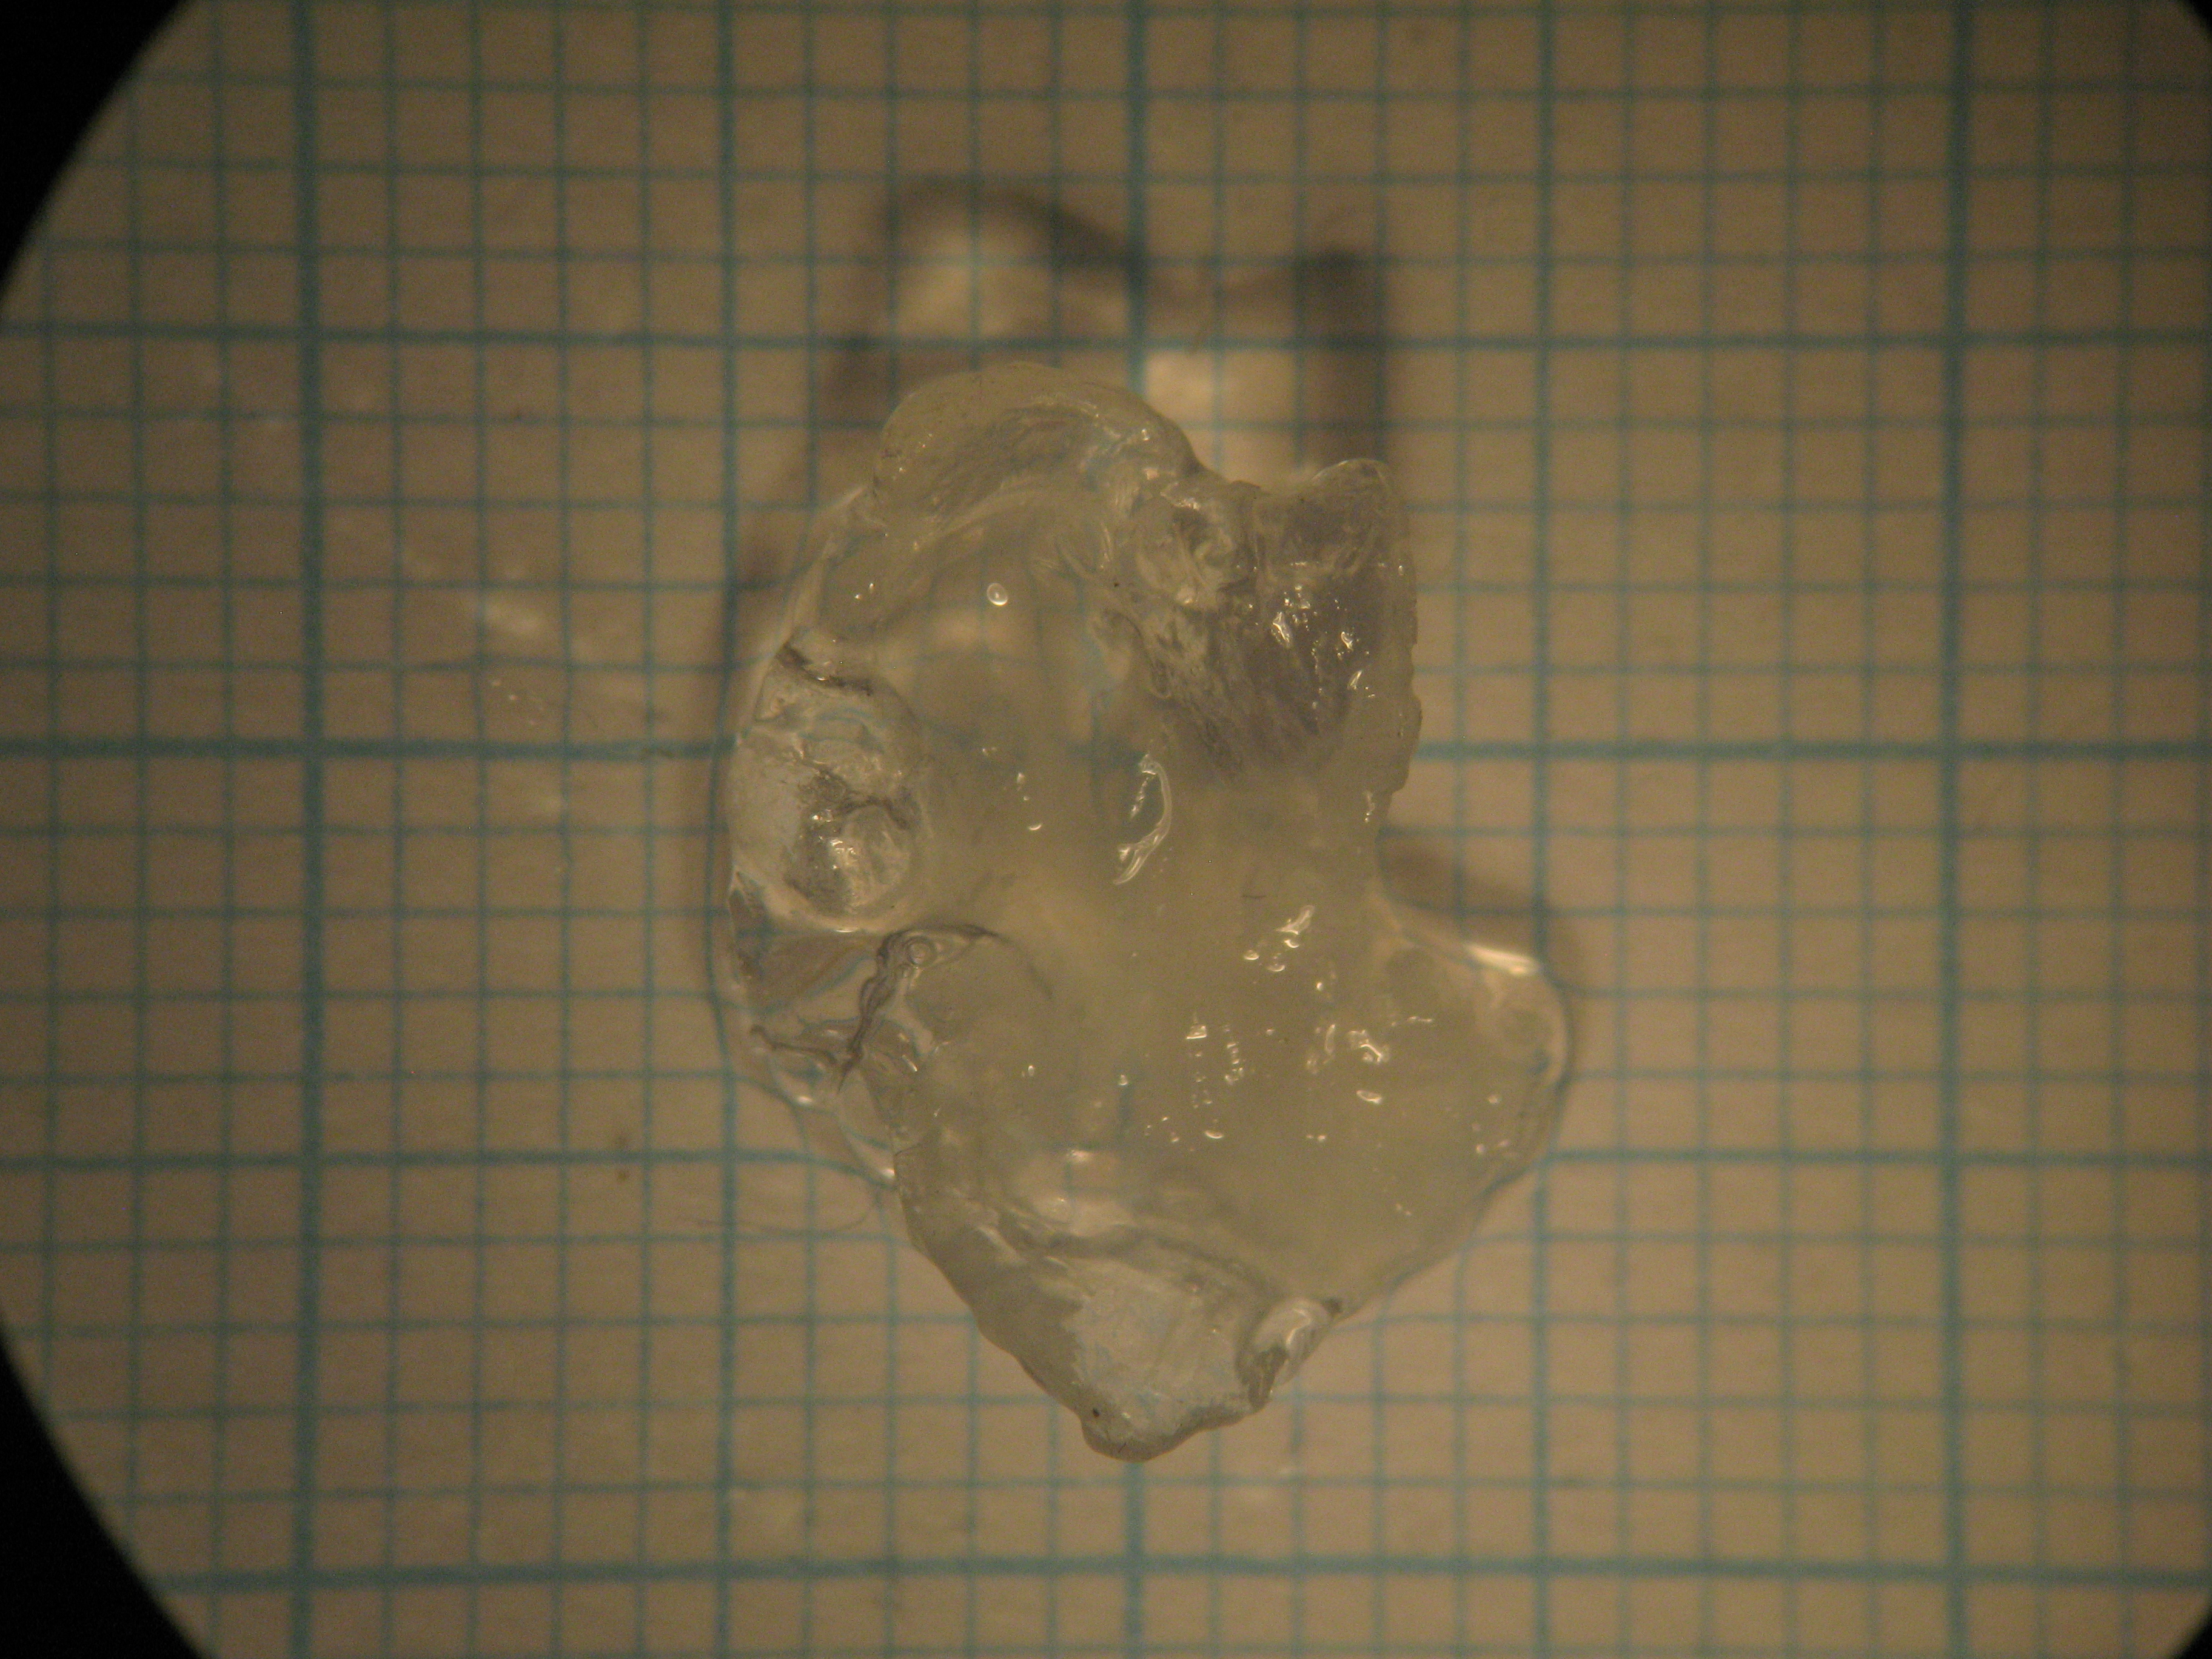
\includegraphics[width=1\linewidth]{Images/SecondSessionWarp.JPG}
    \caption{Tissue curling of CLARITY cleared tissue washed in petri dish (second clearing session)}
    \end{subfigure}
    \medskip
\caption{\textbf{Examples of severe CLARITY sample tissue curling encountered during experimentation.} 1 $mm^2$ grid background for scale.}
    \label{fig:enter-label}
\end{figure}

    
In the first clearing session, samples were stored in 15 mL test tubes for the duration of the washing period. A side effect of this storage method was that many of the samples contoured to match the curve of the tube walls or of the tube's conical end. When removed from these tubes to document expansion, the samples would retain these curled shapes, making lateral expansion documentation impossible to photograph (seen in Figure 3.16(a)). Forcibly flattening thin and healthy cardiac slice samples using pipette tips and slides would allow some to be placed into in a flattened state, but scarred and thicker samples with severe curling could not be flatten without breaking the sample apart in the process.  

To prevent this issue from occurring again, the second session saw the washing step utilize petri dishes instead of test tubes for long term storage. While this change did reduce the occurrence of tissue curling, a minority of samples were still impacted enough to render them unusable for expansion analysis (as seen in Figure 3.16(b)). It is believed these samples contoured to the cylindrical walls of the petri dish, but as these samples were the final samples population to be cleared using CLARITY, there were no further opportunities to test further measures to prevent this curling from occurring. Possible remedies could include washing the samples inside the mounts used for imaging or laying a cover slip of equal diameter to the washing petri dish atop the sample in solution. This would likely prevent any curling from occurring but simultaneously would also extend the washing process by months due to the reduced contact and motion the sample would have in the washing solution. For time limitations this was not attempted in this project but could be tested in future trials as a possible remedy to the issue.

This curling phenomenon caused additional issues when mounting CLARITY samples into the custom designed mount spacers as they made insertion into mounts far more challenging to complete without damaging the sample. Even when uncurled, the tissue would apply pressure on the slides they were placed in as they try to return to their curled states, applying strain against the slides that could cause astigmatisms and aberrations to form in the acquired images as a direct result. This is an issue already inherently present in the design of the sliced tissue imaging mounts (see Chapter 4.3), which is only exacerbated by this additional pressure applied by the uncurled samples. 

\subsubsection{Introduction of CUBIC-RA}
At the start of this project, the use of CUBIC-L/RA was not even considered for use with the cardiac tissue samples. At the time, only CLARITY was being performed and was the only method attempted which had produced viable results. An additional protocol, SHIELD, was also explored as a potential alternative to CLARITY but was quickly abandoned due to poor results and tissue shrinkage results in cleared samples becoming unusable. 

It was during the long washing period of the second round of CLARITY tissue clearing that CUBIC-L/RA was discovered and shown to be a viable alternative to CLARITY. The CUBIC family of hyper-hydrating protocols sacrifices high quality tissue clearing for a significantly reduced processing time and complexity compared to CLARITY (~1 month for a 500 $mm^3$ section of LV wall with CUBIC-L/RA vs ~8 months for a 60 $mm^3$ LV transmural slice). While the reduction in tissue clearing quality would undoubtedly reduce the resolution and penetration of the light sheet into thicker samples, prior results obtained by implementing the protocol with human and  murine heart samples showed the viability of enhanced CUBIC protocols for use in the mesoscale imaging of cardiac tissue \cite{sands_its_2022,tainaka_chemical_2018}. CUBIC-L/RA was recommended by the developers of the CUBIC protocol CUBICStars as being superior to prior versions of the protocol such as CUBIC-1/2, which itself was already shown to be very capable of clearing murine cardiac tissue \cite{sands_its_2022, ueda_cubic_nodate}. 

There was hesitation and concern at the start by collaborators and myself to risk valuable time and tissue sample resources towards testing the viability of this protocol in the developing imaging pipeline, but I persisted in my efforts to implement this process into the research underway. I showcased the viability of the process by performing CUBIC-L/RA clearing on a small, spare cardiac tissue sample leftover from the second round of CLARITY tissue clearing. The tissue proceeded to follow the image acquisition and data processing steps for sliced mounted tissues (see chapter 2,4) and the resulting image acquired of the tissue is shown in Figure 3.17.

\begin{figure}[H]
    \centering
    \includegraphics[width=1\linewidth]{Images/FirstCUBIC.png}
    \caption{\textbf{First CUBIC-L/RA cleared image of cardiac tissue acquired via the imaging pipeline.} Used as proof of concept for introduction of CUBIC-L/RA into imaging pipeline development. 500 micron thick healthy cardiac sample, stained with WGA/AF-488. Scale Bar = 500 microns.}
    \label{fig:enter-label}
\end{figure}

The results of this sample supported the adoption of CUBIC-L/RA into regular use for the purposes of this project, and towards the end of it had surpassed CLARITY as the clearing method of choice due to its higher reliability, shorter processing time, and easier handling of cleared tissue compared to CLARITY. As will be shown in the chapter 5, CUBIC-L/RA was the method of choice for the majority of research projects in which the imaging pipeline was implemented, with only one project utilizing the CLARITY as it had already been underway before my introduction of CUBIC-L/RA had occurred. Had I not introduced CUBIC-L/RA to the project, there would have only been sufficient time to perform this one CLARITY-based experiment with the imaging protocol as opposed to the three experiments to be soon discussed. 


\subsection{Additional Observations}
\subsubsection{\textit{PLA Hydrolysis in CUBIC-L Solution}}

During the course of experimentation, a small test was performed to examine the possibility of using custom made 3D printed mounts with the CUBIC-L immersion of tissue slices undergoing CUBIC-L/RA clearing protocol. As CUBIC-L/RA protocol does not cause heterogeneous expansion in cardiac tissue like CLARITY, the use of the mount in the clearing process was not necessary and thus not included in methodologies for clearing using CUBIC-L/RA. Still, this was seen as a possible variation of the pipeline that may be attempted by future users who would want to mount samples into position for imaging before clearing, thus the scenario merited some investigation to determine viability. 

For this test, a set of mounts were prepared as they would be in the CLARITY protocol and immersed in CUBIC-RA for a period of 3 weeks, stored inside an incubator with stirring. At the end of this period, it was discovered upon closer examination that the chemical composition of CUBIC-L had severely degraded the structural integrity of mount by degrading the PLA material used in their fabrication. Images of this degradation are shown in the Figure 3.18:

\begin{figure}[H]
\centering
\begin{subfigure}[t]{0.4\textwidth}
    \centering
    \includegraphics[width=1\linewidth]{Images/PLA_CUBIC_A.jpg}
    \caption{Severely damaged remains of PLA mount after clearing attempt}
    \end{subfigure}
    ~
    \begin{subfigure}[t]{0.4\textwidth}
    \centering
    \includegraphics[width=1\linewidth]{Images/PLA_CUBIC_B.jpg}
    \caption{CUBIC-L solution saturated With PLA dye after clearing attempt}
    \end{subfigure}
    \medskip

\label{fig:enter-label}
\caption{\textbf{Degradation of 3D printed, PLA mount after exposure to CUBIC-L.} Mounted sample stored immersed in CUBIC-L for 21 Days at 37 degrees Celsius with gentle agitation.}
\end{figure}

Upon further research, it was determined that the N-butyldiethanolamine contained within the CUBIC-L was responsible for this result. The hydroxyl and amine groups of the chemical dissolved in the solution acted as a catalyst which accelerated the hydrolysis of the PLA, breaking down the material at the weakest points, splintering the material into the individual layers created by the 3D printing process \cite{elsawy_hydrolytic_2017}. This rate of degradation was likely only further accelerated by the high temperatures and stirring experienced by the mounts during the clearing time period. 

It was also observed in this test that a significant amount of dye from the PLA had also begun to leech into the clearing solution as the it had acquired a green hue in line with the original colour of the PLA material used by the test mounts (Figure 3.18(b)). This dissolved dye in the solution could cause a wide variety of complications to the clearing process should samples be exposed to it while immersed in CUBIC-L. Avoiding this outcome was seen as a top priority in any instance the mounts were used in the pipeline, thus all mounts fabricated after this test utilized natural coloured PLA containing no dyes for colouration as a precaution. It is recommended that dye free PLA be used for all mounts made for use at any point in the imaging pipeline. While no such dye contamination occurred when the mount is used in the CLARITY clearing and imaging, it is still a possibility worth avoiding altogether. 

\section{Chapter Summary}

This chapter detailed the pre-processing protocols implemented on all cardiac tissues examined throughout the course of this project. The discussion thereafter moved towards the subsequent tissue slicing performed on sliced tissue samples utilized followed by the two tissue clearing protocols utilized in this project: CLARITY and CUBIC-L/RA. To confirm clearing was completed properly and that the tissue structure had not been compromised by the clearing process, characterization experiments were performed for samples cleared using both techniques. Experimental results showed the tissue expansion, transparency, and structural preservation in samples cleared were found to be consistent with results seen in prior publications \cite{olianti_optical_2021, sands_its_2022, epp_optimization_2015, giardini_mesoscopic_2021}. With the clearing protocols validated and tissue samples structure preserved for use in structural analysis post-clearing, the discussion turns to the means by which these samples are to be attached on the mesoSPIM microscope system. The design, installation, characterization, and data processing of the custom designed tissue mounting apparatuses is the focus of the next chapter and is the lynch pin by which the clearing and imaging steps of the imaging pipeline come together.




\chapter{Mounted Cardiac Sample Imaging Experimentation}

Experimentation conducted to accommodate the mesoSPIM microscope imaging of sliced and left ventricle  section samples of leporine cardiac tissue will be detailed in this chapter. Emphasis will be placed on the mounting experimentation conducted for sliced tissues due to the greater number of technical challenges faced compared to mounting LV section samples which are a better fit to the kind of three dimensional, mesoscale sized samples the system was originally designed to handle.  

The characterization of mesoscale images captured, using different designs for both sliced and LV section samples, will showcase the significant impact mount design can have on the quality of sliced tissue images obtained in the system. It is because of this impact that much attention was made through the course of experimentation on finding the optimal dimensional configurations and additive 3D printing settings/designs to achieve the mount fabrication precision necessary to successfully image tissues with minimal aberrations or astigmatisms in the generated image stacks.

\section{Tissue Mounting Methodologies}
\subsection{Sliced Tissue Sample Mounting}

The challenge faced in the mounting of sliced cleared tissues stems from the fact that the mesoSPIM system was designed for the imaging of mesoscale, structurally rigid, three dimensional samples []. This makes use of the system to image thin, structurally plastic, sliced samples complicated to achieve. To successfully image sliced samples utilizing the mesoSPIM system, the following requirements must be met by the method in which a sample is mounted onto the system in order for successfully structural imaging to proceed: 

\begin{itemize}
    \item Prevents the occurrence of motion artifacts as the sample moves in highly viscous RIMS
    \item Eliminates warping of the sample that emerges from CLARITY tissue clearing process
    \item Keeps samples immersed in RIMS without risk of leak, contamination or evaporation.
    \item Removes air pockets, bubbles which can negatively impact the imaging of the sample
\end{itemize}

To this end, 3D printed spacer mounts were utilized to mount sliced tissues. The use of Poly-lactic Acid (PLA) 3D print fabrication allowed for cost effective, mass production of multiple mounts of identical quality in short time periods compared to the metal milling or plastic casting methods available. Fast, high throughput fabrication of mounts was also essential to allow for multiple mount design iterations to be tested concurrently alongside previously established mount designs. This iteration of the design and printer settings utilized allowed for fine adjustment of both to obtain optimal results in short time spans. The process of continued mount design iterating was conducted until the end product was found via image characterization testing to reliably and sufficiently address the aforementioned challenges faced when imaging sliced tissues. 

The mount designs used in all sliced tissue data acquired and presented here will de detailed in the following section. All mount iterations, including those tested but not used for data acquisition through the course of this project are detailed in Appendix A. This includes discussion of changes made between each major generation of mount design leading to the final design selected for use in the imaging pipeline.


\subsubsection{\textit{Finalized Custom 3D Printed Spacer Design}}

\begin{figure}[H]
    \centering
    \includegraphics[width=0.5\linewidth]{Figures/0.4mm B4 Schematic v1.pdf}
    \caption{\textbf{Schematics of finalized mount design.} Mount shown is 0.4 mm internal spacer version. Designs with 0.5, 1.0, and 2.0 mm internal spacers available in Appendix A. Schematics created using Autodesk Fusion 360 software.}
    \label{fig:enter-label}
\end{figure}

The schematic and photo shown in Figure 4.1 is the finalized design of the spacer mount created for use in the imaging pipeline. Schematics for the mounts of this design with 0.5, 1.0, and 2.0 mm internal spacers are provided in Appendix A. 3D printer scripts to fabricate these mounts are available in [INSERT GITHUB URL HERE].

\subsubsection{\textit{Sliced Tissue Mounting Assembly Protocol}}

Once tissues in the imaging pipeline have completed all necessary or desired tissue staining, fixation, and washing (see Chapter 5 for protocols) the cleared tissues are placed into sealed containers wrapped in aluminium foil to protect the light sensitive fluorescent dye (if any) inside the sample.  Samples are then transported to a wet lab area adjacent to the mesoSPIM system for preparation to image. 

Lights are dimmed to the lowest possible level I could safely work in and the samples are removed from containers into a petri dish. Protective coat and gloves were put on before then proceeding with the following step by step protocol for the mounting of cleared slices into the custom designed 3D printed spacers:

\begin{figure}[H]

\begin{subfigure}{.4\linewidth}
  \includegraphics[width=\linewidth]{Images/Step1.jpg}
  \caption{Spread Drop of EI Solution onto slide }
  \label{MLEDdet}
\end{subfigure}\hfill 
~ 
\begin{subfigure}{.4\linewidth}
  \includegraphics[width=\linewidth]{Images/Step2.jpg}
  \caption{Lay tissue slice flat atop EI drop on slide}
  \label{energydetPSK}
\end{subfigure}\hfill 

\medskip 
\begin{subfigure}{.4\linewidth}
  \includegraphics[width=\linewidth]{Images/Step3.jpg}
  \caption{Spread second drop of EI on top of slice}
  \label{velcomp}
\end{subfigure}\hfill 
~
\begin{subfigure}{.4\linewidth}
  \includegraphics[width=\linewidth]{Images/Step4.jpg}
  \caption{Lay second slide atop, avoiding bubbles}
  \label{estcomp}
\end{subfigure}\hfill 

\end{figure}

\clearpage

\begin{figure}[H]
    \addtocounter{figure}{-1}

\begin{subfigure}{.4\linewidth}
\addtocounter{subfigure}{4}
  \includegraphics[width=\linewidth]{Images/Step5.jpg}
  \caption{Slide sandwiched sample into mount with internal spacer placed between the slides}
  \label{velcomp}
\end{subfigure}\hfill 
~
\begin{subfigure}{.4\linewidth}
  \includegraphics[width=\linewidth]{Images/Step6.jpg}
  \caption{Attach mixing nozzle, pipette tip to syringe, fill with dual-component silicone}
  \label{estcomp}
\end{subfigure}\hfill 

\medskip
\begin{subfigure}{.4\linewidth}
  \includegraphics[width=\linewidth]{Images/Step7.jpg}
  \caption{Add mixed silicone at mount frame edges, let dry 10-15 minutes}
  \label{velcomp}
\end{subfigure}\hfill 
~
\begin{subfigure}{.4\linewidth}
  \includegraphics[width=\linewidth]{Images/Step8.jpg}
  \caption{Repeat step (g) on opposite side of mount, confirm both sides fully dried}
  \label{estcomp}
\end{subfigure}\hfill 
    
\begin{subfigure}{.4\linewidth}
  \includegraphics[width=\linewidth]{Images/Step9.jpg}
  \caption{Insert mount topper over open end of mount, ensure fully inserted}
  \label{velcomp}
\end{subfigure}\hfill 
~
\medskip
\begin{subfigure}{.4\linewidth}
  \includegraphics[width=\linewidth]{Images/Step10.jpg}
  \caption{Inject RI Matching Solution slowly via syringe port. Inject till sample immersed.}
  \label{estcomp}
\end{subfigure}\hfill 

\end{figure}

\clearpage

\begin{figure}[H]
    \addtocounter{figure}{-1}

\begin{subfigure}{.4\linewidth}
\addtocounter{subfigure}{10}
  \includegraphics[width=\linewidth]{Images/Step11.jpg}
  \caption{Insert Cap over syringe ports using pliers, ensure fully inserted}
  \label{velcomp}
\end{subfigure}\hfill 
~
\medskip
\begin{subfigure}{.4\linewidth}
  \includegraphics[width=\linewidth]{Images/Step12.jpg}
  \caption{Place mount into light protected storage for duration of RI matching period (12-24hrs).}
  \label{estcomp}
\end{subfigure}\hfill 

 \caption{\textbf{Slice Tissue Mount Assembly Procedure.} Procedure is performed with gloves to prevent smears on quartz glass, contamination of cleared samples. Mount topper marked with red and blue marks to distinguish front and back of mount for imaging.}
    \label{fig:enter-label}
\end{figure}

The protocol described in Figure 4.2 used quartz slides cleaned beforehand with ethanol solution and deionized water. Slides re-cleaned with optical cleaning tissues after mount assembly for optimal imaging. Syringe needles are disposed of in sharps bin and any EasyIndex solution residue is thoroughly cleaned using isopropanol solution. Mixing nozzles used in this protocol were 3D printed and are available on the project GITHUB repository (URL HERE). Mounts under fabrication were placed carefully in cardboard boxes with lids closed for steps requiring drying of silicone to occur to completion.



\subsection{Left Ventricle Sample Mounting}
\subsubsection{\textit{Custom 3D Printed Inner Cuvette Holder Design}}

To attach a rectangular cuvette onto the suspended sample gantry requires the development of an adapter capable of attaching the cuvette to a magnetic Thorlabs kinematic base (Thorlabs KB25/M) without risk of the cuvette detaching from the mount or cracking as a result of excessive stress applied by the mount onto the cuvette. Preliminary 3D printed, PLA mount designs consisted of a simple mount adapter that would use two nylon M2.5 screws inserted on one side of the mount to pin the cuvette wall between the flatten screw tips and the internal surface of the mount that reached partway into the cuvette internal volume. Persistent issues with this design included frequent failures of the screws to hold the sample in place and the gradual reduction in static friction over a period of time due to repeated insertion and removal of the cuvette. Damage to the walls of the cuvette were also frequent as a result of overly tight placement of nylon screws. This would lead to the formation of tension cracks on the cuvette walls.

To eliminate these issues, an additional component was added to the mount adapter: A custom designed, 3D printed base platform. This component, shown below in Figure 4.2(a), is placed beneath the cuvette, holding it in place with a rectangular notch on the platform surface. The platform attaches to the mount via four columns located at each corner of the cuvette. The columns span the height of the cuvette and connect to the upper half of the mount (Figure 4.2(b)) using M2.5 screws. The addition of this component, which avoids direct contact with the cuvette walls to suspend from above, allows for the mounting of the cuvette to occur with minimal risk of damage to the cuvette or detachment from the sample gantry. 

\begin{figure}[H]
    \centering
    \begin{subfigure}[b]{0.6\textwidth}
    \centering
    \includegraphics[width=1\linewidth]{Figures/Updated_Swing_Suspension Cuvette Topper Drawing v1.pdf}
    \caption{Schematic of inner cuvette mount topper}
    \end{subfigure}
    \medskip
    
    \begin{subfigure}[c]{0.6\textwidth}
    \centering
    \includegraphics[width=1\linewidth]{Figures/Updated_Swing_Suspension Cuvette Swing v1.pdf}
    \caption{Schematic of mount suspension harness}
    \end{subfigure}
    \medskip

    \begin{subfigure}[d]{1\textwidth}
    \centering
    \includegraphics[width=0.25\linewidth]{Images/AssembledMountCUBIC.jpg}
    \caption{\textbf{Fully assembled inner cuvette suspension mount containing cardiac sample and CUBIC-RA solution.}}
    \label{fig:enter-label}
    \end{subfigure}

    \caption{\textbf{Final custom internal cuvette mount and attached suspension platform design for use in mesoSPIM microscope.} Schematics to scale, available in Appendix A.}
\end{figure}


\subsubsection{\textit{Left Ventricle Inner Cuvette Mounting}}

CUBIC-L cleared Left Ventricle samples are placed gently into an optical glass cuvette (Portmann Instruments, UG-205 with the epicardium and endocardium facing the longer sides of the cuvette. The internal volume of the cuvette is then filled to two-thirds full of CUBIC-RA solution. 

The custom designed 3D printed mount holder is then inserted onto the top of the solution filled cuvette. A set of 4 screws (2.5M) are then installed into the bore holes located at the top of suspension platform on opposite sides of the cuvette. These bore holes have corresponding screw bores located on the mount holder that connects the components together. Once installed, the suspension platform holds the cuvette in position with minimal risk of slipping or detaching from the holder. Details and schematics of the inner cuvette holder and suspension platform can be found in Appendix A. 

Once the mount and platform are attached and secured, the sample is left to Refractive Index match to the solution for 10-14 days at room temperature. The sample is concealed from light sources for the duration of this period and is secured in place using soft foam to prevent movement without risking scratching the cuvette walls. RI matching is determined to be complete once the opacity homogenizes and colouration changes from orange to pale yellow colour throughout. Tissues nearing the end of homogenization will also lose any buoyancy in the solution seen at the start of immersion. An example of this completion of RI matching compared to the start of CUBIC-RA immersion can be seen in the figure below:

\begin{figure}[H]
    \centering
    \begin{subfigure}[t]{0.5\textwidth}
        \centering
        \includegraphics[width=0.8\linewidth]{Images/PreRA.jpg}
        \caption{Start of CUBIC-RA immersion (day 0)}
    \end{subfigure}%
    ~ 
    \begin{subfigure}[t]{0.5\textwidth}
        \centering
        \includegraphics[width=0.8\linewidth]{Images/PostRA.jpg}
        \caption{End of CUBIC-RA immersion (day 14)}
    \end{subfigure}
    \caption{\textbf{CUBIC-RA refractive index matching of LV samples in glass cuvette at start (a) and end (b) of immersion period}. $1mm^2$ grid paper background for scale.}
\end{figure}

\section{Mounted Sample Imaging Characterization}

To quantify and compare the imaging capabilities of the mesoSPIM system to other, more established microscopy methods, a measurement of samples of known dimension and structure would have to be made and recorded using the system. The ability of the system to successfully discern and accurately measure these samples under conditions experienced by tissue samples when mounted inside the system is essential to validate the microscopy techniques used in the imaging pipeline presented here. As such, fluorescent labelled micro-spheres embedded in agarose are utilized to demonstrate the accuracy of the system in recording micron-scale structural targets. This test will also confirm the proper assembly and alignment of the mesoSPIM system  by being able to replicate spatial resolution limits previously reported in other publications using more traditional inner cuvette mounting methods []. These inner cuvette agarose bead samples can also be used to compare the differences in system characterizations between the CLARITY and CUBIC-L/RA protocols as well as serving as a baseline to which alterations to the imaging, mounting protocol can be compared against.

The main alterations to the imaging protocol made in the development of the imaging pipeline were done to de-skew the images captured from oblique positioned sliced samples (see Chapter 2, Section 3.2). Alterations to the imaging and processing protocols will allow samples to be digitally reconstructed to appear as they would have if they were imaged at a non-oblique angle, which is required for proper histological analysis to be performed. The ability of these custom protocols were validated by comparing the control characterization of micro-spheres embedded in agar mounted using a traditional cuvette to those mounted using the custom 3D printed mounts. These custom mounted agarose micro-bead samples were, in turn, characterized with shear and no shear techniques to determine how well mechanical de-skewing protocols are able to replicate non-oblique oriented mounting when processed. 


\subsection{Fluorescent Micro-spheres in 1\% Agarose Sample Fabrication} 

\subsubsection{\textit{Agarose Samples in Custom 3D Printed Spacers}}

Two quartz slides are cleaned thoroughly using lens cleaning tissues and then promptly inserted into the custom made, cleared tissue 3D printed mount. Once slotted into place, Eco-Sil Speed Addition Curing Silicone (Picodent®, PIC. 13001000), is thoroughly mixed before then being injected onto the edges of the mount viewing window, ensuring a watertight seal is formed. One side of the mount is fully sealed and left to dry for 20-25 minutes at room temperature. This step is then repeated on the opposite side and left to dry. 

Once the epoxy is fully dry on both sides of the mount, 1\% agarose in deionized $H_2O$ solution is prepared in a sealable microwave safe glass jar by mixing 19.8 mL of deionized $H_2O$ is mixed with 0.2 grams of low gelling temperature agarose (Sigma Aldritch, A9414-25G). The solution is then mixed thoroughly by hand for a minute until the solution is opaque with no large clumps of agarose remaining. The jar lid is then removed and the solution placed into a 800 Watt microwave oven and heated at the medium setting for 60 seconds. The solution is monitored, and the microwave heating is manually stopped once the solution begins to consistently boil. The solution should now be clear in appearance with no clumps or opaque regions visible.

After the solution ceases boiling, the heated jar is carefully removed from the microwave using oven gloves and it is left to cool on the counter-top for 5 minutes. While cooling, 5 uL of 1.04 um Dragon Green fluorescent beads (Bang Laboratories, FSDG004) is measured using a pipette to then be injected into the solution at the end of the cooling period. The jar is sealed closed with the lid and the solution is stirred again for 1 minute by hand. 

After stirring the agarose bead solution, a 0.4 $\mu$m diameter syringe is filled with the liquid solution and injected into the mounts between the slides. The mounts are filled half-way with the bead solution. Once filled, the mount topper is placed on the top of the mounts and the solution is left to cool and gelatinize for 15-20 minutes at room temperature. Once the topper is checked to be firmly in place, a syringe is used to inject EasyIndex\texttrademark\ (EI) Solution (LifeCanvas Technologies, EI-500-1.52) into the remaining empty volume above the agarose gelatin in the mount. A syringe port and air exhaust are built into the topper to allow for simultaneous injection of solution into the mount and expulsion of air out to prevent pressure build ups. Once the mount is filled to the top using EI solution, a lid is inserted over the injection and exhaust ports to prevent dust and debris from entering. The bead sample is then left to immerse in the EI solution for 12-24 hours to permit full perfusion of the solution across the agarose gelatin. Bead samples are then imaged following mounted tissue slice imaging protocols (see chapter 2, section 3).

\subsubsection{\textit{Agarose Samples in Internal Cuvettes}}

For 1\% Agarose Solution Bead Samples to be used in the characterization of the mesoSPIM system using a mounted inner cuvette, the same solution protocol that was documented for samples in 3D printed spacers was followed (See section 2.1 of this chapter). Once the beads are mixed into the solution and sufficiently cooled, the solution is poured into 2 rectangular cuvettes: 1 Quartz (Portmann Instruments UQ-205) and 1 Optical Glass (Portmann Instruments UG-205). Using a plastic 1 mL pipette the bottom third to one-half of the cuvette internal volume is filled (approx.. 2-3.5 mL). The solution is left to cool further and gelatinize for 15-20 minutes. 

After the agarose has set, the cuvette is placed atop a custom designed 3D printed suspension platform. The platform contains a small 1mm deep recess of equal width to the cuvette to ensure secure placement. Once inserted, the remaining internal volume of the optical glass cuvette is filled with CUBIC-RA solution using a plastic pipette and the quartz cuvette is filled with EI solution. Both solutions are added until the meniscus of the solution inside the cuvette is roughly 5mm below the top lip of the cuvette walls (approx. 3.5 mL). 

The custom designed 3D printed mount holder used for left ventricle mounting (see section 1.2 of this chapter) is inserted onto the top of the solution filled cuvette and the remainder of the mounting protocol for this custom mount is followed as previous detailed. The agarose inner cuvette sample proceeds to undergo the inner cuvette imaging protocol previous detailed in chapter 2, section 3. The image stack recorded is set to [INSERT PARAMETERS HERE]. 

\subsection{Customized Image Processing For Oblique Imaging}

With the orientation of the sample being angled at 45 degrees, a method is required to process these images stacks to return them back to a non-oblique orientation. The two methods utilized to achieve this outcome (with and without shearing) will use the following descriptions for axes of orientation: 

\begin{itemize}
    \item At the 0 degree orientation, the sample is parallel to the plane of excitation pathway (x-axis) and perpendicular to the plane of the detection pathway (z-axis) of the mesoSPIM. This will be referred to as the 'system coordinate system' and will be defined here on out as: (\textit{x,z}). 
 
 \item At an 45 degree orientation, the x and z planes of the sample are now translated 45 degrees counter-clockwise from the x,z planes of the system coordinate system. These new axes of orientation will be referred to as the 'sample coordinate system' and will be defined here on out as: (\textit{x',z'}).
\end{itemize}

Python scripts utilized to perform the following oblique image processing techniques can be found in the following Githup repository: [GITHUB URL HERE].

 
\subsubsection{\textit{Sheared Volume Reconstruction}}

A diagram detailing the sheared process of volume reconstruction is shown in Figure 4.6. This sheared method has been previously implemented for use in LSM systems such as OPM and iSPIM and has been modified for use here in the mesoSPIM [SEE PAPER REFS,x2]. 

\begin{figure}[H]
    \centering
    \includegraphics[width=1\linewidth]{Figures/shear.png}
    \medskip
    \caption{\textbf{Sheared scanning of oblique oriented sample for volume reconstruction [].} Diagram legend: Image stack regions occupied by sample volume (cyan); Image stack regions occupied by empty pixels (gray), additional empty pixels added in processing (light gray). Direction of sample movement in the system (magenta arrow) indicated with respect to the system coordinate system.}
    \label{fig:enter-label}
\end{figure}

In this method, as the oblique sample is shifted in z-axis of the system coordinate system, the resulting image series will be sheared as the sample is seen to shift across the camera field of view (Figure 4.6(1-2)) with large blank spaces, void of any signal, found on either side of the sample in every tile and in the stitched image once tiles are combined (4.6(2-3)). These empty regions are an unavoidable consequence of the oblique orientation as only a cross-section of the sample is seen in each frame of the imaging stack. Once acquired, the sheared stack undergoes affine transformation which rotates and scales the data from each frame in the stack, mapping each pixel from the system coordinate system into the sample coordinate system. This process requires the addition of even more regions of empty pixel data to allow digital reorientation of the image stack to occur (Figure 4.6(4-5)). Once reoriented, the sample is reconstructed remaining sheared in the x' and z' axes (Figure 4.6(6)).


\subsubsection{\textit{No-Shear Volume Reconstruction}}

A diagram detailing the no shear process of volume reconstruction is shown in Figure 4.6. This no-sheared method was created during the course of this project in collaboration with primary advisor Dr.Caroline Muellbroich and research colleagues Dr. Sharika Mohanan, Dr. Erin Boland, and Mr. Ahmed Elnageh [Cite Publication]. 

\begin{figure}[H]
    \centering
    \includegraphics[width=1\linewidth]{Figures/noshear.png}
    \medskip
    \caption{\textbf{No shear scanning of oblique oriented sample for volume reconstruction [].} Diagram legend: Image stack regions occupied by sample (cyan), Image stack regions occupied by empty pixels (gray). Direction of sample movement in the system (magenta arrow) indicated with respect to the system coordinate system.}
    \label{fig:enter-label}
\end{figure}

 The no shear methods activates the x and z axis stages to shift the sample in both axes simultaneously in equal measure between each image captured by the system (Figure 4.7(1)). This movement is in line with the 45 degree orientation of the sample, which shifts the sample to the right in equal amount to shift in the z-axis (Tan 45\degree = 1/1). By shifting the sample in both x and z , the region of the camera FOV occupied by the sample remains unchanged across the entire image stack. To further enhance the axial resolution, the distance traversed by the ETL across the camera FOV during axial scanning protocol is programmed to instead now only span the narrow central region occupied by the tissue []. By decreasing the span of the viable beam region, the central width of the beam is able to be narrowed even further than what is normally achievable using traditional cuvettes, theoretically allowing for even higher resolution than possible when imaging using standard mesoSPIM operation techniques.
 
 Once fully acquired, the Non-sheared Data Stacks are stitched together, rotated 90 degrees, and cropped to isolate the sample from empty pixel regions (Figure 4.7(3-5)). As the sample volume pixels are consistently located in the same region in all frames, the camera FOV regions crop settings are identical in size and position in all frames, expediting the process. Once cropped, the data is scaled on x' axis using affine transform, leaving only the z' axis sheared.

\subsection{Agarose Bead Sample Characterization Results}

Analysis of all Agarose bead samples utilized point spread analysis programs created and optimized by Mr. Ahmed Elnageh in python script []. Coding scripts are available in [GITHUB URL, folder location]

\subsubsection{\textit{CLARITY Mount Results}}
\paragraph{Mounted Inner Cuvette}
To provide a control data set to compare data obtained using the custom designed mounts, the spatial resolution of the mesoSPIM using established protocols and mounting methods such as an internal quartz cuvette were recorded and analysed using point spread analysis techniques. The results of this analysis are shown in the following figure.

\begin{figure}[H]
    \centering
     \begin{tikzpicture}
            \begin{axis}
            [
            scale = 1,
            xmin = 1.5,
            xmax = 8.5,
            ylabel={Spatial Axis},
            xlabel={Recorded Measurement (microns)},
            ytick={1,2,3},
            yticklabels={Z,Y,X}, 
            boxplot/box extend=0.25,
            ]
    
    \addplot+ [boxplot] 
            table [y index=0] {Data/rect_cuvette/zfwhm.txt}
            [above]
            node at
              (boxplot whisker cs:\boxplotvalue{lower whisker},1)
              {\pgfmathprintnumber{\boxplotvalue{lower whisker}}}
            node at
              (boxplot box cs: \boxplotvalue{median},1)
              {\pgfmathprintnumber{\boxplotvalue{median}}}
            node at
              (boxplot whisker cs:\boxplotvalue{upper whisker},1)
              {\pgfmathprintnumber{\boxplotvalue{upper whisker}}}
            ;
            
    \addplot+[boxplot] 
            table [y index=0] {Data/rect_cuvette/yfwhm.txt}
            [above]
            node at
              (boxplot whisker cs:\boxplotvalue{lower whisker},1)
              {\pgfmathprintnumber{\boxplotvalue{lower whisker}}}
            node at
              (boxplot box cs: \boxplotvalue{median},-1)
              {\pgfmathprintnumber{\boxplotvalue{median}}}
            node at
              (boxplot whisker cs:\boxplotvalue{upper whisker},1)
              {\pgfmathprintnumber{\boxplotvalue{upper whisker}}}
            ;
            
    \addplot+[boxplot] 
            table [y index=0] {Data/rect_cuvette/xfwhm.txt}
            [above]
            node at
              (boxplot whisker cs:\boxplotvalue{lower whisker},1)
              {\pgfmathprintnumber{\boxplotvalue{lower whisker}}}
            node at
              (boxplot box cs: \boxplotvalue{median},-1)
              {\pgfmathprintnumber{\boxplotvalue{median}}}
            node at
              (boxplot whisker cs:\boxplotvalue{upper whisker},1)
              {\pgfmathprintnumber{\boxplotvalue{upper whisker}}}
            ;
                       
            \end{axis}
        \end{tikzpicture}
    \caption{\textbf{[ADD UNITS]Point spread analysis: Quartz glass cuvette, florescent beads in agarose solution} Box plots of full width at half maximum (FWHM) of 1 micron florescent beads dimensions measured in recording (n = 1278 beads).}
    \label{fig:enter-label}
\end{figure}


The average FWHM of the recorded sub-resolution beads in the x,y, and z axes were calculated to be 3.95$\pm$0.8 microns, 5.22$\pm$1.06 microns, and 5.96$\pm$0.75 microns respectively [DOUBLE CHECK]. This data is consistent with previous examinations of spatial resolution of the mesoSPIM using similar mounting techniques[].

\paragraph{Sheared Vs No Shear}
Next, the spatial resolution of the mesoSPIM using the new custom made mounts in combination with shear and no shear protocols were recorded and analysed using point spread analysis techniques. Both protocols were performed using 4 separate agarose solution filled mounts to ensure the results acquired using the custom designed mounts are repeatable with minimal differences in achievable resolution between each mount. The results of the no shear recordings were collected and are compared side by side in Figure 4.9 (a-d):

\begin{figure}[H]
\centering
    \begin{subfigure}[t]{0.46\textwidth}
        \centering
        \begin{tikzpicture}
            \begin{axis}
            [
            scale = 0.9,
            xmin = 2,
            xmax = 13,
            ytick={1,2,3},
            yticklabels={Z',Y, X'}, 
            ylabel={Spatial Axis},
            xlabel={Recorded Measurement (microns)},
            boxplot/box extend=0.25,
            ]
    
    \addplot+ [boxplot] 
            table [y index=0] {Data/B4_2/2zfwhm.txt}
            [above]
            node at
              (boxplot whisker cs:\boxplotvalue{lower whisker},1)
              {\pgfmathprintnumber{\boxplotvalue{lower whisker}}}
            node at
              (boxplot box cs: \boxplotvalue{median},1)
              {\pgfmathprintnumber{\boxplotvalue{median}}}
            node at
              (boxplot whisker cs:\boxplotvalue{upper whisker},1)
              {\pgfmathprintnumber{\boxplotvalue{upper whisker}}}
            ;
            
    \addplot+[boxplot] 
            table [y index=0] {Data/B4_2/2yfwhm.txt}
            [above]
            node at
              (boxplot whisker cs:\boxplotvalue{lower whisker},1)
              {\pgfmathprintnumber{\boxplotvalue{lower whisker}}}
            node at
              (boxplot box cs: \boxplotvalue{median},-1)
              {\pgfmathprintnumber{\boxplotvalue{median}}}
            node at
              (boxplot whisker cs:\boxplotvalue{upper whisker},1)
              {\pgfmathprintnumber{\boxplotvalue{upper whisker}}}
            ;
            
    \addplot+[boxplot] 
            table [y index=0] {Data/B4_2/2xfwhm.txt}
            [above]
            node at
              (boxplot whisker cs:\boxplotvalue{lower whisker},1)
              {\pgfmathprintnumber{\boxplotvalue{lower whisker}}}
            node at
              (boxplot box cs: \boxplotvalue{median},-1)
              {\pgfmathprintnumber{\boxplotvalue{median}}}
            node at
              (boxplot whisker cs:\boxplotvalue{upper whisker},1)
              {\pgfmathprintnumber{\boxplotvalue{upper whisker}}}
            ;
                       
            \end{axis}
        \end{tikzpicture}
        \caption{\textbf{Agarose Bead Mount \#1 (n = 1185)}}
    \end{subfigure}
    \medskip
    \hspace{1em}
    ~
    \begin{subfigure}[t]{0.46\textwidth}
        \centering
        \begin{tikzpicture}
             \begin{axis}
            [
            scale = 0.9,
            xmin = 2,
            xmax = 13,
            ytick={1,2,3},
            yticklabels={Z',Y, X'},
            ylabel={Spatial Axis},
            xlabel={Recorded Measurement (microns)},
            boxplot/box extend=0.25,
            ]
    
    \addplot+ [boxplot] 
            table [y index=0] {Data/B4_3/3zfwhm.txt}
            [above]
            node at
              (boxplot whisker cs:\boxplotvalue{lower whisker},1)
              {\pgfmathprintnumber{\boxplotvalue{lower whisker}}}
            node at
              (boxplot box cs: \boxplotvalue{median},-1)
              {\pgfmathprintnumber{\boxplotvalue{median}}}
            node at
              (boxplot whisker cs:\boxplotvalue{upper whisker},1)
              {\pgfmathprintnumber{\boxplotvalue{upper whisker}}}
            ;
            
    \addplot+[boxplot] 
            table [y index=0] {Data/B4_3/3yfwhm.txt}
            [above]
            node at
              (boxplot whisker cs:\boxplotvalue{lower whisker},1)
              {\pgfmathprintnumber{\boxplotvalue{lower whisker}}}
            node at
              (boxplot box cs: \boxplotvalue{median},1)
              {\pgfmathprintnumber{\boxplotvalue{median}}}
            node at
              (boxplot whisker cs:\boxplotvalue{upper whisker},1)
              {\pgfmathprintnumber{\boxplotvalue{upper whisker}}}
            ;
            
    \addplot+[boxplot] 
            table [y index=0] {Data/B4_3/3xfwhm.txt}
            [above]
            node at
              (boxplot whisker cs:\boxplotvalue{lower whisker},1)
              {\pgfmathprintnumber{\boxplotvalue{lower whisker}}}
            node at
              (boxplot box cs: \boxplotvalue{median},-1)
              {\pgfmathprintnumber{\boxplotvalue{median}}}
            node at
              (boxplot whisker cs:\boxplotvalue{upper whisker},1)
              {\pgfmathprintnumber{\boxplotvalue{upper whisker}}}
            ;
            [
                       
            \end{axis}
        \end{tikzpicture}
        \caption{\textbf{Agarose Bead Mount \#2 (n = 407)}}
    \end{subfigure}
    \medskip
    
\begin{subfigure}[t]{0.46\textwidth}
        \centering
        \begin{tikzpicture}
            \begin{axis}
            [
            scale = 0.9,
            xmin = 2,
            xmax = 13,
            ytick={1,2,3},
            yticklabels={Z',Y, X'},
            ylabel={Spatial Axis},
            xlabel={Recorded Measurement (microns)},
            boxplot/box extend=0.25,
            ]
    
    \addplot+ [boxplot] 
            table [y index=0] {Data/B4_4/4zfwhm.txt}
            [above]
            node at
              (boxplot whisker cs:\boxplotvalue{lower whisker},1)
              {\pgfmathprintnumber{\boxplotvalue{lower whisker}}}
            node at
              (boxplot box cs: \boxplotvalue{median},1)
              {\pgfmathprintnumber{\boxplotvalue{median}}}
            node at
              (boxplot whisker cs:\boxplotvalue{upper whisker},1)
              {\pgfmathprintnumber{\boxplotvalue{upper whisker}}}
            ;
            
    \addplot+[boxplot] 
            table [y index=0] {Data/B4_4/4yfwhm.txt}
            [above]
            node at
              (boxplot whisker cs:\boxplotvalue{lower whisker},1)
              {\pgfmathprintnumber{\boxplotvalue{lower whisker}}}
            node at
              (boxplot box cs: \boxplotvalue{median},-1)
              {\pgfmathprintnumber{\boxplotvalue{median}}}
            node at
              (boxplot whisker cs:\boxplotvalue{upper whisker},1)
              {\pgfmathprintnumber{\boxplotvalue{upper whisker}}}
            ;
            
    \addplot+[boxplot] 
            table [y index=0] {Data/B4_4/4xfwhm.txt}
            [above]
            node at
              (boxplot whisker cs:\boxplotvalue{lower whisker},1)
              {\pgfmathprintnumber{\boxplotvalue{lower whisker}}}
            node at
              (boxplot box cs: \boxplotvalue{median},-1)
              {\pgfmathprintnumber{\boxplotvalue{median}}}
            node at
              (boxplot whisker cs:\boxplotvalue{upper whisker},1)
              {\pgfmathprintnumber{\boxplotvalue{upper whisker}}}
            ;
            [
                       
            \end{axis}
        \end{tikzpicture}
        \caption{\textbf{Agarose Bead Mount \#3 (n = 1341)}}
    \end{subfigure}
    \medskip
    \hspace{1em}
    ~
    \begin{subfigure}[t]{0.46\textwidth}
        \centering
        \begin{tikzpicture}
             \begin{axis}
             [
            scale = 0.9,
            xmin = 2,
            xmax = 13,
            ytick={1,2,3},
            yticklabels={Z',Y, X'},
            ylabel={Spatial Axis},
            xlabel={Recorded Measurement (microns)},
            boxplot/box extend=0.25,
            ]
    
    \addplot+ [boxplot] 
            table [y index=0] {Data/B4_5/5zfwhm.txt}
            [above]
            node at
              (boxplot whisker cs:\boxplotvalue{lower whisker},1)
              {\pgfmathprintnumber{\boxplotvalue{lower whisker}}}
            node at
              (boxplot box cs: \boxplotvalue{median},-1)
              {\pgfmathprintnumber{\boxplotvalue{median}}}
            node at
              (boxplot whisker cs:\boxplotvalue{upper whisker},1)
              {\pgfmathprintnumber{\boxplotvalue{upper whisker}}}
            ;
            
    \addplot+[boxplot] 
            table [y index=0] {Data/B4_5/5yfwhm.txt}
            [above]
            node at
              (boxplot whisker cs:\boxplotvalue{lower whisker},1)
              {\pgfmathprintnumber{\boxplotvalue{lower whisker}}}
            node at
              (boxplot box cs: \boxplotvalue{median},1)
              {\pgfmathprintnumber{\boxplotvalue{median}}}
            node at
              (boxplot whisker cs:\boxplotvalue{upper whisker},1)
              {\pgfmathprintnumber{\boxplotvalue{upper whisker}}}
            ;
            
    \addplot+[boxplot] 
            table [y index=0] {Data/B4_5/5xfwhm.txt}
            [above]
            node at
              (boxplot whisker cs:\boxplotvalue{lower whisker},1)
              {\pgfmathprintnumber{\boxplotvalue{lower whisker}}}
            node at
              (boxplot box cs: \boxplotvalue{median},-1)
              {\pgfmathprintnumber{\boxplotvalue{median}}}
            node at
              (boxplot whisker cs:\boxplotvalue{upper whisker},1)
              {\pgfmathprintnumber{\boxplotvalue{upper whisker}}}
            ;
            [
                       
            \end{axis}
        \end{tikzpicture}
        \caption{\textbf{Agarose Bead Mount \#4 (n = 761)}}
    \end{subfigure}
    \caption{\textbf{Agarose bead samples point spread analysis: 4 Custom 3D Printed Mounts, No Shear Technique} Box plots of full width at half maximum (FWHM) results in x',y, and z' sample coordinate axes. Median, upper and lower quartiles, max and min extrema shown (N,overall = 3691 beads)}
    \label{fig:enter-label}
\end{figure}

 The average FWHM results of sheared and no sheared recordings taken of the same agarose bead sample set are compared side by side in Figure 4.10.

\begin{figure}[H] 
    \centering
    \begin{subfigure}[t]{0.46\textwidth}
    \centering
        \begin{tikzpicture}
            \begin{axis}
             [
            scale = 0.9,
            xmin = 2,
            xmax = 15.5,
            ytick={1,2,3},
            yticklabels={Z',Y, X'},
            ylabel={Spatial Axis},
            xlabel={Recorded Measurement (microns)},
            boxplot/box extend=0.25,
            ]

            \addplot+ [boxplot] 
                    table [y index=0] {Data/double/zfwhm.txt}
                    [above]
                    node at
                      (boxplot whisker cs:\boxplotvalue{lower whisker},1)
                      {\pgfmathprintnumber{\boxplotvalue{lower whisker}}}
                    node at
                      (boxplot box cs: \boxplotvalue{median},-1)
                      {\pgfmathprintnumber{\boxplotvalue{median}}}
                    node at
                      (boxplot whisker cs:\boxplotvalue{upper whisker},1)
                      {\pgfmathprintnumber{\boxplotvalue{upper whisker}}}
                    ;
                    
            \addplot+[boxplot] 
                    table [y index=0] {Data/double/yfwhm.txt}
                    [above]
                    node at
                      (boxplot whisker cs:\boxplotvalue{lower whisker},1)
                      {\pgfmathprintnumber{\boxplotvalue{lower whisker}}}
                    node at
                      (boxplot box cs: \boxplotvalue{median},1)
                      {\pgfmathprintnumber{\boxplotvalue{median}}}
                    node at
                      (boxplot whisker cs:\boxplotvalue{upper whisker},1)
                      {\pgfmathprintnumber{\boxplotvalue{upper whisker}}}
                    ;
                    
            \addplot+[boxplot] 
                    table [y index=0] {Data/double/xfwhm.txt}
                    [above]
                    node at
                      (boxplot whisker cs:\boxplotvalue{lower whisker},1)
                      {\pgfmathprintnumber{\boxplotvalue{lower whisker}}}
                    node at
                      (boxplot box cs: \boxplotvalue{median},-1)
                      {\pgfmathprintnumber{\boxplotvalue{median}}}
                    node at
                      (boxplot whisker cs:\boxplotvalue{upper whisker},1)
                      {\pgfmathprintnumber{\boxplotvalue{upper whisker}}}
                    ;
            [
                       
            \end{axis}
        \end{tikzpicture}
    \caption{\textbf{Averaged point spread analysis: Custom 3D printed mount, shear technique} Box plots of average FWHM in examined agarose bead samples (m = 4).}
    \end{subfigure}
    \hspace{2em}
    ~
    \begin{subfigure}[t]{0.46\textwidth}
        \centering
            \begin{tikzpicture}
                 \begin{axis}
                 [
                scale = 0.9,
                xmin = 2,
                xmax = 15.5,
                ytick={1,2,3},
                yticklabels={Z',Y, X'},
                ylabel={Spatial Axis},
                xlabel={Recorded Measurement (microns)},
                boxplot/box extend=0.25,
                ]
        
        \addplot+ [boxplot] 
                table [y index=0] {Data/double/nzfwhm.txt}
                [above]
                node at
                  (boxplot whisker cs:\boxplotvalue{lower whisker},1)
                  {\pgfmathprintnumber{\boxplotvalue{lower whisker}}}
                node at
                  (boxplot box cs: \boxplotvalue{median},-1)
                  {\pgfmathprintnumber{\boxplotvalue{median}}}
                node at
                  (boxplot whisker cs:\boxplotvalue{upper whisker},1)
                  {\pgfmathprintnumber{\boxplotvalue{upper whisker}}}
                ;
                
        \addplot+[boxplot] 
                table [y index=0] {Data/double/nyfwhm.txt}
                [above]
                node at
                  (boxplot box cs:\boxplotvalue{lower whisker},0.9)
                  {\pgfmathprintnumber{\boxplotvalue{lower whisker}}}
                node at
                  (boxplot box cs: \boxplotvalue{median},-1)
                  {\pgfmathprintnumber{\boxplotvalue{median}}}
                node at
                  (boxplot box cs:\boxplotvalue{upper whisker},1)
                  {\pgfmathprintnumber{\boxplotvalue{upper whisker}}}
                ;
                
        \addplot+[boxplot] 
                table [y index=0] {Data/double/nxfwhm.txt}
                [above]
                node at
                  (boxplot whisker cs:\boxplotvalue{lower whisker},1)
                  {\pgfmathprintnumber{\boxplotvalue{lower whisker}}}
                node at
                  (boxplot box cs: \boxplotvalue{median},-1)
                  {\pgfmathprintnumber{\boxplotvalue{median}}}
                node at
                  (boxplot whisker cs:\boxplotvalue{upper whisker},1)
                  {\pgfmathprintnumber{\boxplotvalue{upper whisker}}}
                ;
                [      
                \end{axis}
            \end{tikzpicture}
    \caption{\textbf{Averaged point spread analysis: Custom 3D printed mount, no shear technique} Box plots of average FWHM in examined agarose bead samples (m = 4).}
    \end{subfigure}

    \label{fig:enter-label}
    \caption{\textbf{Point spread analysis comparison: Shear and no shear techniques.} 1 micron florescent beads in agarose solution dimensions measured in recordings: Shear recording (n = 314 beads); No shear recording (n = 3673 beads).}
\end{figure}

Over the 4 custom mount samples created and recorded using the shear technique, the average FWHM of the recorded sub-resolution beads in the x',y, and z' axes were calculated to be 5.94$\pm$0.77 microns, 8.12$\pm$1.32 microns, and 13.23$\pm$0.72 microns respectively. In comparison, the average FWHM of the same 4 custom mount samples recorded using the no-shear technique were calculated to be 4.66$\pm$0.67 microns in x'-axis, 3.86$\pm$0.49 microns in the y-axis, and 7.76$\pm$1.64 microns in the z'-axis.

Between Shear and No Shear techniques, axial resolution (in the z'-axis) is found to double using the no shear method while lateral resolution is seen to have an approximately 30\% increase in the y-axis. Resolution in the x'-axis was found to be similar in both methods as anticipated with both images remaining sheared in that specific axis. Significant overlap is seen in the calculated error margins of x'-axis resolution, though spread of measurements in the no-shear x'-axis data contained slightly less variation.

To quantify changes in resolution anisotropy between shear and no shear, the anisotropy ratio (A) was determined between the FWHM of the x and y axis components of lateral resolution in both averaged data sets. 

\begin{equation}
A = \frac{FWHM_x}{FWHM_y}
\end{equation}
\medskip

The Anisotropy Ratio in the sheared data was found to be at 1.34 while the ratio was 0.61 in the no shear data, indicating the lateral anisotropy had increased in the no-shear recordings as a result of the reduced FWHM value of the y-axis and generally consistent FWHM value found in the x-axis. 

\subsubsection{\textit{CUBIC-L/RA Inner Cuvette Results}}
The spatial resolution of the mesoSPIM using established CUBIC-L/RA protocols and mounting methods such as an internal optical glass cuvette were recorded and analysed using point spread analysis techniques. The results of this characterization are shown in the following figure.

\begin{figure}[H]
    \centering
     \begin{tikzpicture}
            \begin{axis}
            [
            scale = 1,
            xmin = 1.5,
            xmax = 7.5,
            ytick={1,2,3},
            yticklabels={Z,Y,X}, 
            ylabel={Spatial Axis},
            xlabel={Recorded Measurement (microns)},
            boxplot/box extend=0.25,
            ]
    
    \addplot+ [boxplot] 
            table [y index=0] {Data/cubic_cuvette/488nm/zfwhm.txt}
            [above]
            node at
              (boxplot whisker cs:\boxplotvalue{lower whisker},1)
              {\pgfmathprintnumber{\boxplotvalue{lower whisker}}}
            node at
              (boxplot box cs: \boxplotvalue{median},1)
              {\pgfmathprintnumber{\boxplotvalue{median}}}
            node at
              (boxplot whisker cs:\boxplotvalue{upper whisker},1)
              {\pgfmathprintnumber{\boxplotvalue{upper whisker}}}
            ;
            
    \addplot+[boxplot] 
            table [y index=0] {Data/cubic_cuvette/488nm/yfwhm.txt}
            [above]
            node at
              (boxplot whisker cs:\boxplotvalue{lower whisker},1)
              {\pgfmathprintnumber{\boxplotvalue{lower whisker}}}
            node at
              (boxplot box cs: \boxplotvalue{median},-1)
              {\pgfmathprintnumber{\boxplotvalue{median}}}
            node at
              (boxplot whisker cs:\boxplotvalue{upper whisker},1)
              {\pgfmathprintnumber{\boxplotvalue{upper whisker}}}
            ;
            
    \addplot+[boxplot] 
            table [y index=0] {Data/cubic_cuvette/488nm/xfwhm.txt}
            [above]
            node at
              (boxplot whisker cs:\boxplotvalue{lower whisker},1)
              {\pgfmathprintnumber{\boxplotvalue{lower whisker}}}
            node at
              (boxplot box cs: \boxplotvalue{median},-1)
              {\pgfmathprintnumber{\boxplotvalue{median}}}
            node at
              (boxplot whisker cs:\boxplotvalue{upper whisker},1)
              {\pgfmathprintnumber{\boxplotvalue{upper whisker}}}
            ;
                       
            \end{axis}
        \end{tikzpicture}
    \caption{\textbf{Point spread analysis: Optical glass cuvette, florescent beads in agarose solution} Box plots of full width at half maximum (FWHM) of 1 micron florescent beads examined in recording (n = 1278 beads).}
    \label{fig:enter-label}
\end{figure}

The average FWHM of the recorded sub-resolution beads in the x,y, and z axes were calculated to be 4.19$\pm$0.64 microns, 3.85$\pm$0.42 microns, and 4.61$\pm$1.12 microns respectively in the 488 nm channel. This data is consistent with previous examinations of spatial resolution of the mesoSPIM using similar mounting techniques[]. 

\section{Discussion}
The main aim of this series of experiments was to produce an optimized tissue mounting procedure and data processing methodology to obtain unaltered structural data utilizing these novel, 3D printed mounting designs. The results obtained from the experiments described in this chapter confirms that the finalized pipeline protocols described in Chapter 4.1 is fully capable of producing high quality images of ex vivo tissue structure when implemented as part of the overarching tissue imaging pipeline. 

\subsection{Tissue Mounting Discussion}
\subsubsection{\textit{Sliced Tissue Mounting Discussion}}
In the process of designing mounts for the imaging of CLARITY cleared tissue samples, there was a considerable convenience seen in the fact that the mounting frame required for the clearing process (See Chapter 3.1) could also be utilized for imaging with the addition of 3D components to overlay the base mount. Basic resizing of the mount to allow the insertion of slightly wider (0.1-0.2 mm) and thinner (0.05-0.1 mm) quartz slides instead of standard issue microscope soda-lime glass slides used in the CLARITY protocol was the only change required, with all other requirements for the imaging mount (such as being able to be suspended from the sample gantry using a Thorlabs post holder, allowing for the injection of RI matching solution, and being able to be stored for extended periods of time between imaging session) being met by the addition of a Thorlabs post-holder compatible mount topper with sealable syringe injection ports. The simplicity of the design of all three of these components meant modifications can easily be made to allow samples and slides of various width and thickness to be imaged utilizing this imaging process. 

\subsubsection{\textit{Left Ventricle Mounting Discussion}}

Initial designs which used friction applied by nylon screws onto the cuvette walls to suspend the cuvette from the top were abandoned. This method proved to unreliable and was prone to damaging to the cuvette gradually over time. Preserving the condition of the fragile cuvette walls during imaging was made a priority, ensuring no cracks or scratching occurred while the mount was assembled, in use, and when removed after imaging. In the place of the initial design, a new mount design would instead support the cuvette from below with the new bore holes added to the old mount topper design to attach the bottom support frame.

Another factor taken into consideration for the mount's design was the limited volume the cuvette could safely traverse without coming into contact with the sides or base of the outer cuvette installed into the mesoSPIM system. Supports attached to the cuvette from the bottom of the cuvette would reduce the depth the cuvette could be lowered without impacting the outer cuvette base. This same issue holds true for the support frame that must span across the sides of the inner cuvette to connect the base platform to the mount topper. For these reasons, the attachable base platform created for use with the cuvette mount topper was made as thin and narrow as possible while maintaining its ability to support the inner cuvette from beneath. This allows the cuvette to traverse the largest volume in the outer cuvette possible while also keeping the inner cuvette securely affixed to the sample gantry suspended above the detection path.



\subsection{Imaging Characterization Discussion}
A successful mounting and associated data acquisition process was established for use in the imaging pipeline utilizing CLARITY cleared tissue slices. Shearing and aberrations seen from the oblique imaging methods used to record images of sliced samples contained in custom made mounts were compensated for in the data processing conducted on the raw data after acquisition. The adjustments made to the imaging process further aided in reducing the processing demands required to restore the image back to a non-oblique orientation. By implementing the no-shear protocol (see Figure 4.7), the excessive additions of empty pixel data and the affine transformation performed on multiple axis seen in the shear method (See Figure 4.6) were eliminated. In their place, simple image matrix rotation, rescaling, and affine transformation in just one axis is required, streamlining the processing method and reducing the file size of data sets by up to five times in some cases. 

Results from characterization tests performed confirm the no-shear protocols as superior in acquiring higher image quality compared to sheared methods. The axial resolution achievable by the no-shear technique was even found to be roughly double that of the sheared techniques a result of the reduced ETL range of movement, which could not be easily replicated in sheared imaging without significant alteration to the mesoSPIM software.

The recorded z-axis resolutions obtained in these experiments establishes the 2 and 3 microns step sizes to be implemented when recording image stacks of tissue samples using these mounting and image processing techniques. These z-steps signify the distance between each frame recorded by the mesoSPIM and is set to be roughly 50\% of the axial FWHM distance determined for each mounting method, ensuring sufficient sampling of tissue volume is collected during imaging sessions. 


\subsubsection{\textit{Aberration Induced Variability In Mounted Sliced Tissue Characterization}}

The results seen from no-shear characterization were reasonably similar to the resolution and image quality seen in the mesoSPIM system using a more standard sample orientation,\textit{[CONFIRM WHEN YOU GET THE DATA]}. It should be noted though that there does exist variability in the recorded FWHM that changes from one mounted sample to another.

This increased variability within each individual bead sample is a direct result of the aberrations in the images acquired from mounted samples, which varies considerably in prominence and location between each sample. This aberrations are believed to be a direct result of stress and tension applied onto the quartz glass of the mounts by the 3D printed frame and silicone sealant surrounding the mount. These components are believed to apply inward pressure on the outer edges of the quartz while agarose gel within the mounts applies a simultaneous outward force across the surface area of the slide it comes into contact with.

The uneven and spread out application of these forces onto the quartz slides result in isolated, but clearly delineated regions within each sample that contains noticeable astigmatisms and reduced resolution compared to the rest of the sample within the same FOV. An example of one such aberrant region, as well as close look at the effect these aberrations have on individual fluorescent beads, are shown in the figure below:

\begin{figure}[H]
    \centering
    \begin{subfigure}[t]{0.75\textwidth}
        \centering
        \includegraphics[width=0.6\linewidth]{Images/astigma2.png}
        \caption{\textbf{Uneven aberration and astigmatisms in adjacent regions imaged from mounted agarose bead sample.} Scale bar = 200 micron, yellow line marks clear boundary between adjacent normal and aberration regions. Image acquired using ImageJ software.}
    \end{subfigure}
    \medskip
    
    \begin{subfigure}[t]{0.75\textwidth}
        \centering
        \includegraphics[width=0.8\linewidth]{Images/astigma1.png}
        \caption{\textbf{Astigmatism seen in an individual bead In XY, XZ, and YZ planes.} Scale Bars = 5 micron, Yellow Lines Mark Axis Midpoints. Image set acquired by Ahmed Elnageh using ImageJ software}
    \end{subfigure}
        
    \caption{\textbf{Image aberrations encountered during system characterization testing.} Overview image (A) and individual bead images (B).}
\end{figure}

Several measures and modifications were made to the design of the mounts (see Appendix 1) and the application of the silicone sealant was streamlined and made consistent across all samples mounted to mitigate the severity of these astigmatisms and aberrations in the images acquired. While these measures were unable to eliminate the issue entirely, the streamlining and optimization of the mount design and mounting protocol were able to reduce the variability of the issue and allow for more consistent characterization results to be acquired, allowing for more effective post-processing mitigation of optical aberrations to be performed. 

In addition to the external force applied by the quartz glass against the mount frame, it is anticipated that any warping or curling of the tissue held within the mount (see Chapter 3.3.2) will contribute additional force onto the surface of the slides as the flattened out tissue will press against the quartz glass as it tries to return to its curled state. While this additional force was not present in bead samples used for characterization testing, it remains a possibility that compounds the importance of avoiding any such curling in cleared tissue sample from occurring during implementation of this imaging pipeline.

\subsubsection{\textit{Considerations On Data Processing}}

One considerable advantage seen in the no shear processing method compared to the shear method is the considerable reduction in processing time and file sizes that results from the no shear method. Comparisons in file sizes and processing times are shown in Figure 4.12.

\begin{figure}[H]
    \centering
        \begin{subfigure}[t]{0.4\textwidth}
        \centering
        \begin{tikzpicture}
                \begin{axis}
                [
                scale = 0.85,
                xlabel = Raw Data File Size (GB),
                ylabel = Processed Data File Size (GB),
                xmin = 0,
                xmax = 18,
                ymax= 40,
                ymin = 0
                ]
                \addplot table {Data/Noshearfilesize.tex}
                ;
                \addplot table {Data/Shearfilesize.tex}
                        ; 
                \end{axis}
            \end{tikzpicture}
        \caption{\textbf{Change in file size of data after image processing}.}
        \label{fig:enter-label}
        \end{subfigure}
        \hspace{2em}
        ~
        \begin{subfigure}[t]{0.4\textwidth}
        \centering
         \begin{tikzpicture}
                \begin{axis}
                [
                scale = 0.85,
                xlabel = Input File Size (GB),
                ylabel = Processing Time (s),
                xmin = 0,
                xmax = 14,
                ymax= 300,
                ymin = 0
                ]
                \addplot table {Data/NoShearTime.tex}
                ;
                \addplot table {Data/ShearTime.tex}
                ; 
                \end{axis}
            \end{tikzpicture}
        \caption{\textbf{Change in affine transform processing time to input file size}.}
        \label{fig:enter-label}
        \end{subfigure}
    \caption{\textbf{Comparison of data processing files size and processing times}. Blue lines indicate trend for no shear data, red lines indicates trend for shear data.}
    \label{fig:enter-label}
\end{figure}

In comparison to the sheared processed data files, which increases in sizes by a factor of 4.24$\pm$0.07 (average$\pm$SD) , the no shear processed data files actually reduces the size of the original raw data file by a factor of 0.75$\pm$0.004. This leads to the file size of shear processed files being larger than the no-shear data files by a factor of 5.63$\pm$0.10. 

With regard to processing times, the sheared data on average was able to perform the affine transformation on the raw data at a rate of 22.53$\pm$0.33 milliseconds per GB. In comparison, the no shear process was able to perform the same image processing task at a faster rate with an average processing time of 13.32$/pm$0.18 milliseconds per GB. This equates to the no shear processing reducing the time required to process images by a factor of 1.69$\pm$0.03 compared to shear method.

These findings are of particular importance as the limited memory storage space in the PC operating the mesoSPIM proved to be a considerable challenge that can delay the recording and processing of data if not properly managed in a timely manner. To resolve this issue, any and all means by which the amount of memory and processing time required for a given tissue could be reduced without sacrificing image fidelity should be explored and implemented. Further discussion of specific measures considered throughout this project will be detailed in Chapter 6.

\section{Chapter Summary}

The final piece of the cardiac tissue imaging pipeline, customized sample mounting and data processing, was detailed in the first half of this chapter. The second half details the characterization experiments used to determine the achievable axial and lateral resolutions using inner cuvettes for both CLARITY and CUBIC-L/RA. In addition, the custom mounting and data processing methods (shear, no shear) used for CLARITY cleared slices were characterize to determine the loss in image fidelity incurred as a result of the oblique imaging methods deployed. The results obtained showed the no shear method of volume reconstruction of oblique mounted tissues as the superior method compared to sheared method. This is due to the no shear methods improving resolution in all spatial axes and allowing for the processing of image data with greater speed and smaller file sizes compared to sheared processing. As such, no shear data processing will be utilized in all subsequent analysis of cleared cardiac tissue. This, along with the rest of now fully described tissue imaging pipeline, will prove instrumental in the next chapter. Chapter 5 will present three cardiovascular research projects in which the completed and characterized cardiac tissue imaging pipeline was implemented from start to end, demonstrating the feasibility of utilizing the pipeline in current and future research into cardiac tissue structure.
\chapter{Cardiac Tissue Imaging Pipeline Applications In Research}

Previous chapters have demonstrated the ability of the developed cardiac tissue clearing, mounting, and imaging protocols to be combined into a single tissue processing pipeline. This pipeline was then shown to be capable of producing high resolution images of cardiac tissue structure. The post-processing of these image stacks allows for an accurate volumetric reconstruction of the myocardium sample to be generated for use in structural analysis. Now remains two major questions that need to be answered to validate the pipeline as a technique meriting standard, general use in cardiophotonics research: 
\begin{itemize}
    \item How can this pipeline data be utilized in cardiac structural analysis? 
    \item How versatile can the pipeline data be in biological research?
\end{itemize}

This chapter will seek to answer these questions by examining three instances in which the pipeline was successfully implemented into an experimental protocol. In doing so, they showcase how this imaging data can be implemented in quantitative examination of myocardial tissue, confirming the usability and versatility of data acquired by the processing pipeline.

These biological research projects were conducted in conjunction with the University of Glasgow’s School of Cardiovascular and Metabolic Health (SCMH), which implemented the processing pipeline and utilized the mesoSPIM microscope system assembled in School of Physics and Astronomy (PH\&A). Modifications made to the tissue staining portion of pipeline allowed these projects to obtain unique image data sets from cleared cardiac tissue. 

The first project seeks to obtain volumetric data from the innervation in cardiac tissue post myocardial infarction. The second project utilized the imaging pipeline to determine the optimal combination of fluorescent stains for use in histological analysis of left ventricle (LV) samples. The third and final project seeks to examine the ability of implanted spheroids to connect with the surrounding cardiac tissue. In all three cases, desired physiological data is dependent on the preservation of volumetric tissue structure. This data is impractical to obtain in experimental set ups using traditional, two-dimensional cardiac histology methods and can be addressed through implementation of the tissue processing pipeline.


\section{Innervation of Post-MI Leporine Hearts}
This project was conducted in collaboration with Dr. Erin Boland at the School of Cardiovascular and Metabolic Health, College of Medical, Veterinary, and Life Sciences, University of Glasgow. Steps 1-5 in the tissue processing pipeline (See Figure 2.1) were conducted by Dr. Boland and myself with subsequent imaging and data post processing completed by both me, Dr. Sharika Mohanan, and Mr. Ahmed Elnageh using Fiji ImageJ and IMARIS software. 

Methodology, data, and results acquired for this project currently under peer review for subsequent publication by advisor and paper lead author Dr. Caroline Mullenbroich at time of thesis submission. 

\subsection{Experimental Concepts}
\subsubsection{\textit{Background}}
The objective of this project is to obtain both structural and electrophysiological data from leporine heart models both healthy and post MI. This data will be used to test the hypothesis that cardiac remodelling post MI will result in alterations to the myocardium innervation. Structural and functional datasets obtained from samples will be correlated to determine associations between structural formations and electrical activity in the organ. Obtaining these correlated sets of data will allow changes to the sympathetic innervation that occurs because of tissue remodelling post-myocardial infarction to be documented and analysed further in research settings [].


Currently established methods of examining sympathetic innervation in cardiac tissue provide only limited spatial and morphological detail from existing histology methods requiring tissue slices no greater than 10 microns in thickness to conduct []. It is hypothesized that the combination an optimized tissue clearing pipeline with innervation targeted labelling of cardiac tissue samples will permit faster acquisition with greater spatial resolution, simpler image reconstruction, and higher structural preservation than previously possible in established histological assessments.

\subsubsection{\textit{Methodologies}}

For this experiment, 8 leporine hearts (New Zealand White Rabbits) underwent functional data recording attached to Langendorff perfusion set up. the imaging pipeline utilizing CLARITY tissue clearing protocol (See Chapter 3) was subsequently implemented on 10 tissue slices (0.5 mm and 1.0 mm thickness) extracted from the LV wall of functional data recorded heart models. (N,total = 10; n, healthy = 3; n, scar = 7). 

\paragraph{Staining}

Samples then initially underwent staining protocols based on previously published procedures along with guidelines provided by the antibody manufacturers []. Adjustments to the protocol were implemented based on the results achieved using this base protocol with multiple concentrations and combinations of fluorescent, antibody stains. These adjustments aimed to improve florescent signal intensity, reduce background noise, and ensure sufficient and homogeneous stain penetration into the tissue volume. Stains that aim to florescence specific structures in the tissue, such as cell nuclei or tissue innervation, were also examined to ensure labelling in these channels remained specific with every adjustment made to the initial protocol. The finalized staining protocol created is described with precise timing steps with timings and volumes in Table 5.1:

\begin{table}[H]
    \centering
    \begin{tabular}{cc}
        \textbf{Procedure Step} & \textbf{Time Duration}\\
            \medskip
         1. PBS Washing & 3 Hours\\
             \medskip
         2. PBS-T Washing & 24 Hours\\
            \medskip
         3*. 1:200 Anti-TH Antibody Wash in PBS-T at $4\celsius$ & 72 Hours\\
            \medskip
         4. 1:100 WGA/AF-488 Conjugate Stain Wash & 48 Hours\\
            \medskip
         5*. 1:200 Goat anti-mouse AF 647 Secondary Antibody Wash in PBS-T & 48 Hours\\
            \medskip
         6. 1:1000 DAPI Nuclear Stain Wash in PBS-T & 6 Hours**\\
            \medskip
         6. PBS-T Wash (3x) & 8 Hours (x3)\\
            \medskip
         7. 4\% PFA/PBS Wash & 15 Min\\
            \medskip
         8. PBS Washes (x3) & 5 Min (3x)\\
            \medskip
    \end{tabular}
    \medskip
    \caption{\textbf{Finalized antibody/WGA conjugate dual staining protocol for CLARITY cleared tissue slices.} All steps performed with gentle agitation at Room Temperature (RT) unless otherwise stated. Steps 3-8 are light sensitive, performed with light shielding around sample at all times. *Antibody staining steps skipped if DAPI utilized. **DAPI can be added to last 6 hours of prior washing step, step skipped if antibody staining performed.}
    
\end{table}


After optimization of staining to the best of our ability, two 0.5mm thick, CLARITY cleared tissue slice samples were stained using two unique staining combinations Dr. Erin Boland and myself. 

The first tissue was stained with a combination of WGA/AF-488 and the nucleic acid stain DAPI, which followed the protocol presented in Table 5.1 but with the antibody staining steps omitted with nuclear dye staining steps performed in their place. The second tissue was stained with WGA/AF-488 and the antibody anti-Tyrosine hydroxylase (Anti-TH; ThermoFisher MA5-32984) following the same staining protocol with antibody staining steps intact. 

\paragraph{Image Acquisition}

Stained tissues were mounted by myself according to the imaging pipeline sliced tissue mounting procedures (see Chapter 4) and imaged according to mesoSPIM mounted sliced tissue protocols (see Chapter 2). The entire tissue volume of each sample was recorded across multiple image stack tiles stitched together using BigStitcher software package on Fiji ImageJ software \cite{horl_bigstitcher_2019}. The python script implemented for the point spread analyses of agarose bead samples in Chapter 4 was again applied to two regions of interest (ROIs) in the tissue sample stained with WGA/AF-488 and DAPI (see INSERT GITHUB URL) to analyse cell nuclei that could be discerned in the recorded and no-shear processed image of the tissue produced. 

\paragraph{Data Processing}

Image reconstruction is performed on data collected from this sample to determine if the staining protocol in combination with the greater imaging pipeline is capable of discerning the fragile and intricate fibre-like network of nerve cells, which distinguishes myocardial innervation, across the cleared tissue sample \cite{saltzman_biomedical_2015}. The qualitative examination of the reconstructed volume from the oblique scanned, no-shear processed images will determine if the process can be implemented on a larger scale to perform more quantitative analysis of the intricate remodelling of cardiac tissue innervation in post-MI tissue samples compared to non MI, healthy controls. 

Point spread analysis is performed using signal acquired from cell nuclei in the sample to validate the no shear processing method as capable of reconstructing images from oblique scans with sufficient resolution and image quality to discern, count, and calculate densities of cell nuclei across the sample. Point spread analysis process created and optimized by Mr. Ahmed Elnageh in python script (available in [GITHUB URL, folder location]). Successful completion of this quantitative analysis with results mirroring estimates for nuclei number and density expected in cardiac tissue samples is used to confirm if a given tissue is viable for use in biological histology. 




\subsection{Experimental Results}
\subsubsection{\textit{Nuclear Stain, No Shear Imaging Analysis}}

Upon completion of image processing, a full volume reconstruction of the sliced tissue was generated in the Fiji ImageJ software \cite{schindelin_fiji_2012}. The figure on the next page showcases signal acquired from DAPI and WGA-AF 488 stains within a single imaging frame, within a single frame of the reconstructed volume, approximately 0.25 mm beneath the surface of the tissue slice.

\begin{figure}[H]
\centering
\begin{subfigure}[t]{0.9\textwidth}
\includegraphics[width=1\linewidth]{Images/Fig5_1.png}
\caption{\textbf{Stitched image of 0.5 mm leporine cardiac tissue slice cleared with CLARITY and stained using WGA/AF-488 and DAPI.} Scale Bar = 5 mm. Magenta channel (405 nm), cyan channel (488 nm).}
\end{subfigure}
\medskip

\begin{subfigure}[t]{0.475\textwidth}
\centering
\includegraphics[width=0.75\linewidth]{Images/ROI1.png}
\caption{\textbf{ROI \#1.} Highlighted in cyan in (a), Scale Bar = 300 microns.}
\end{subfigure}
\medskip
~
\begin{subfigure}[t]{0.475\textwidth}
\centering
\includegraphics[width=0.75\linewidth]{Images/ROI2.png}
\caption{\textbf{ROI \#2.} Highlighted in pink in (a), Scale Bar = 300 microns.}
\end{subfigure}
\caption{\textbf{Results of no-shear image processing in combination with tissue imaging pipeline processes.} Tissue orientated at 45 degree angle with respect to detection, excitation pathways. Light sheet is orientated perpendicularly with respect to the reconstructed, de-skewed images shown above.}
\end{figure}

As seen in Figure 5.1, the no shear method of data processing in combination with the adapted dual fluorescent dye staining protocol was able to produce images of tissue structure with sufficiently high resolution and contrast to distinguish individual cell nuclei and membranes across the 0.5 mm thick cardiac tissue slice with homogenous visibility of cell nuclei located within the densely packed fibres of the myocardium. These nuclei in selected ROIs from the DAPI emission channel were measured according to the sample coordinate system (x',y ,z'; see Chapter 4.2.2) and the distribution of measurements in each axis for each ROI is shown on the following page:

\begin{figure}[H]
\centering
    \begin{subfigure}[t]{0.49\textwidth}
        \centering
        \begin{tikzpicture}
            \begin{axis}
            [
            scale = 1,
            ytick={1,2,3},
            yticklabels={Z',Y, X'},
            xlabel={Axis},
            ylabel={Recorded Bead Dimension (microns)},
            boxplot/box extend=0.25,
            xmax = 25,
            xlabel = {Length ($\mu$m)}
            ]
    
   \addplot+[boxplot, mark=none] 
            table [y index=0] {Data/ROI1/zfwhm.txt}
            [above]
            node at
              (boxplot whisker cs:\boxplotvalue{lower whisker},1)
              {\pgfmathprintnumber{\boxplotvalue{lower whisker}}}
            node at
              (boxplot box cs: \boxplotvalue{median},-1)
              {\pgfmathprintnumber{\boxplotvalue{median}}}
            node at
              (boxplot whisker cs:\boxplotvalue{upper whisker},1)
              {\pgfmathprintnumber{\boxplotvalue{upper whisker}}}
            ;
            
    \addplot+[boxplot, mark=none] 
            table [y index=0] {Data/ROI1/yfwhm.txt}
            [above]
            node at
              (boxplot whisker cs:\boxplotvalue{lower whisker},1)
              {\pgfmathprintnumber{\boxplotvalue{lower whisker}}}
            node at
              (boxplot box cs: \boxplotvalue{median},1)
              {\pgfmathprintnumber{\boxplotvalue{median}}}
            node at
              (boxplot whisker cs:\boxplotvalue{upper whisker},1)
              {\pgfmathprintnumber{\boxplotvalue{upper whisker}}}
            ;
   \addplot+[boxplot, mark=none] 
            table [y index=0] {Data/ROI1/xfwhm.txt}
            [above]
            node at
              (boxplot whisker cs:\boxplotvalue{lower whisker},1)
              {\pgfmathprintnumber{\boxplotvalue{lower whisker}}}
            node at
              (boxplot box cs: \boxplotvalue{median},-1)
              {\pgfmathprintnumber{\boxplotvalue{median}}}
            node at
              (boxplot whisker cs:\boxplotvalue{upper whisker},1)
              {\pgfmathprintnumber{\boxplotvalue{upper whisker}}}
            ;
            \end{axis}
 
        \end{tikzpicture}
        \caption{\textbf{ROI 1 (n=43)}}
    \end{subfigure}
    \medskip
    ~
    \begin{subfigure}[t]{0.49\textwidth}
        \centering
        \begin{tikzpicture}
           \begin{axis}
            [
            scale = 1,
            ytick={1,2,3},
            yticklabels={Z',Y, X'},
            boxplot/box extend=0.25,
            xmax = 25,
            xlabel = {Length ($\mu$m)}
            ]
    
   \addplot+[boxplot, mark=none] 
            table [y index=0] {Data/ROI2/zfwhm.txt}
            [above]
            node at
              (boxplot whisker cs:\boxplotvalue{lower whisker},1)
              {\pgfmathprintnumber{\boxplotvalue{lower whisker}}}
            node at
              (boxplot box cs: \boxplotvalue{median},-1)
              {\pgfmathprintnumber{\boxplotvalue{median}}}
            node at
              (boxplot whisker cs:\boxplotvalue{upper whisker},1)
              {\pgfmathprintnumber{\boxplotvalue{upper whisker}}}
            ;
            
    \addplot+[boxplot, mark=none] 
            table [y index=0] {Data/ROI2/yfwhm.txt}
            [above]
            node at
              (boxplot whisker cs:\boxplotvalue{lower whisker},1)
              {\pgfmathprintnumber{\boxplotvalue{lower whisker}}}
            node at
              (boxplot box cs: \boxplotvalue{median},-1)
              {\pgfmathprintnumber{\boxplotvalue{median}}}
            node at
              (boxplot whisker cs:\boxplotvalue{upper whisker},1)
              {\pgfmathprintnumber{\boxplotvalue{upper whisker}}}
            ;
   \addplot+[boxplot, mark=none] 
            table [y index=0] {Data/ROI2/xfwhm.txt}
            [above]
            node at
              (boxplot whisker cs:\boxplotvalue{lower whisker},1)
              {\pgfmathprintnumber{\boxplotvalue{lower whisker}}}
            node at
              (boxplot box cs: \boxplotvalue{median},-1)
              {\pgfmathprintnumber{\boxplotvalue{median}}}
            node at
              (boxplot whisker cs:\boxplotvalue{upper whisker},1)
              {\pgfmathprintnumber{\boxplotvalue{upper whisker}}}
            ;
            
            \end{axis}
        \end{tikzpicture}
        \caption{\textbf{ROI 2 (n=133)}}
    \end{subfigure}
    \caption{\textbf{Distribution of cell nuclei dimensional measurements.} Median, upper and lower quartiles, max and min extrema shown. Measurements recorded in sample coordinate system (x', y, z').}
    \label{fig:enter-label}
\end{figure}

The FWHM of cell nuclei measurements in both ROIs were compared to the resolution limits established by the agarose bead characterization experiments. The comparison in distribution of these axial dimension measurements are presented in Figure 5.3: 

\begin{figure}[H]
        \centering
        \begin{tikzpicture}
            \begin{axis}
            [
            scale = 1,
            ytick={1,2,3},
            yticklabels={$Z'_{ROI_2}$,$Z'_{ROI_1}$,\empty},
            xlabel={Axis},
            ylabel={Recorded Bead Dimension (microns)},
            boxplot/box extend=0.25,
            xmin= 6,
            xmax = 18, 
            ymin = 0,
            ymax=3,
            xlabel = {Length ($\mu$m)}
            ]
    
     \addplot+[boxplot, mark=none] 
            table [y index=0] {Data/ROI2/zfwhm.txt}
            [above]
            node at
              (boxplot box cs: \boxplotvalue{median},1.1)
              {\pgfmathprintnumber{\boxplotvalue{median}}}
            ;
    \addplot+ [boxplot prepared={lower whisker=13.23, upper whisker=13.23,whisker extend = 4,draw position=1,every whisker/.style={magenta,ultra thick}}] 
                %table [y index=0] {Data/double/zfwhm.txt}
                coordinates {};
                    %;
    \addplot+ [boxplot prepared={lower whisker=7.76, upper whisker=7.76,whisker extend = 4,draw position=1,every whisker/.style={cyan,ultra thick}}]
                %table [y index=0] {Data/double/zfwhm.txt}
                coordinates {};
                    %;
    \addplot+[boxplot, mark=none] 
            table [y index=0] {Data/ROI1/zfwhm.txt}
            [above]
            node at
              (boxplot box cs: \boxplotvalue{median},1.1)
              {\pgfmathprintnumber{\boxplotvalue{median}}}
            ;
              \end{axis}
        \end{tikzpicture}
        \caption{\textbf{FWHM distribution of cell nuclei axial measurements in ROIs (Fig. 5.1(a-b)).} (N, ROI \#1 = 27 nuclei; N, ROI \#2 = 132 nuclei)  Median axial measurement, inner quartiles, minimum and maximum values are shown. magenta line = shear imaging method axial resolution limit (13.23 microns). Cyan line = no shear method axial resolution limit (7.76 microns).}
    \end{figure}

It was seen in this comparison of axial data that the resolution required to properly discern cell nuclei in the axial dimension is higher than the average resolution limit established in characterization tests for sliced sample mounting using the shear technique. The majority of nuclei in ROI \#1 (Fig. 5.1(b)) could be discerned by the shear method, including the second through fourth quartiles of nuclei recorded. In ROI \#2, however, only the fourth and upper half of the third quartile of recorded nuclei could have been resolved as the remainder of nuclei in the ROI were out of the shear method's axial resolution range. This is in stark contrast to the no-shear method's axial resolution limit, which was capable of resolving a larger range of cell nuclei sizes, which in the myocardium can span from 5 to 15 microns in width []. With only a small number of nuclei recorded falling below the no-shear resolution limit in ROI \#2, and the inner quartiles of recorded nuclei in both ROIs falling well above the resolution limit, the application of the no shear technique was considered successful in identifying and measuring the general population of cell nuclei in cardiac tissue processed and imaged through the imaging pipeline.

\subsubsection{\textit{Anti-TH Immunolabelling, No Shear Imaging Analysis}}

For the tissue sample stained utilizing WGA/AF-488 and anti-TH antibody immunostaining, the volume of the tissue sample was reconstructed utilizing BigStitcher software programme on Fiji ImageJ \cite{horl_bigstitcher_2019}. Anti-TH immunostaining will target the neuronal structural contained within the sample and the images recorded, emitting the highest level of signal in those regions of the sample in which the innervation of the myocardium remains intact. The following figure showcases signal acquired from the Anti-TH and WGA/AF-488 stains within a section of the reconstructed volume containing the highest density regions of signal seen from the anti-TH channel.  

\begin{figure}[H]
    \centering
    \includegraphics[width=1\linewidth]{Images/Anti_TH_Overview2.png}
    \caption{\textbf{Overview image frame of 0.5 mm leporine cardiac tissue slice cleared with CLARITY and stained using WGA/AF-488, Anti-TH Antibody Staining.} Scale bar = 1000 microns. 647 and 488 excitation channels overlaid, colour-inverted using Fiji ImageJ Software. Cyan dotted line marks boundary of tissue volume fluoresced by WGA/AF-488, Red dotted line marks boundary of tissue volume densely fluoresced by anti-TH. Light sheet is orientated perpendicularly with respect to the reconstructed imaging planes shown above.}
\end{figure}
\medskip

 The individual image channels for WGA/AF-488 and Anti-TH is provided in Figure 5.5. Select ROIs, for zoomed in looks at cell morphological details visible in each channel, are also provided besides the images of their respective imaging channels of origin.

\begin{figure}[H]
    \begin{subfigure}[t]{0.5\textwidth}
    \includegraphics[width=1\linewidth]{Images/wga_channel.png}
    \caption{\textbf{WGA/AF-488 channel of image frame.} Scale bar = 1000 microns.}
    \end{subfigure}
    \medskip
    ~
    \begin{subfigure}[t]{0.45\textwidth}
    \centering
    \includegraphics[width=0.8\linewidth]{Images/wga_zoomin.png}
    \caption{\textbf{ROI \#1 (Highlighted in white in (a)).} Scale bar = 250 microns.}
    \end{subfigure}
    \medskip
    
    \begin{subfigure}[t]{0.5\textwidth}
    \includegraphics[width=1\linewidth]{Images/anti_Th_channel.png}
    \caption{\textbf{Anti-TH channel of image frame.} Scale bar = 1000 microns.}
    \end{subfigure}
    \medskip
    ~
    \begin{subfigure}[t]{0.45\textwidth}
    \centering
    \includegraphics[width=0.8\linewidth]{Images/anti_th_zoomin.png}
    \caption{\textbf{ROI \#1 (Highlighted in white in (c)).} Scale bar = 250 microns.}
    \end{subfigure}
    \medskip
    
\caption{\textbf{Individual channels and zoomed in ROIs of 0.5 mm leporine cardiac tissue slice cleared with CLARITY and stained using WGA/AF-488, anti-TH antibody staining.} Image processing performed by Dr. Sharika Mohanan. Signal intensity (value: 0 (yellow) - 255 (red/blue)). Profiles in yellow-blue (WGA/AF-488) and yellow-red (anti-TH). Light sheet is orientated perpendicularly with respect to the imaging planes shown above.}
\end{figure}

3D reconstructions of the innervation pathways seen in selected ROIs across the images tissue volume were assembled and are shown on the next page (Fig. 5.6(b-c)) with colour highlights marking the ROI locations in the Anti-TH Overview Image (Fig 5.6(a)).

\begin{figure}[H]
    \centering
    \begin{subfigure}[t]{0.6\textwidth}
    \includegraphics[width=1\linewidth]{Images/antith_roi_overview.png}
    \caption{\textbf{Anti-TH channel of image frame.} Scale bar = 50 micron. Signal intensity profiles in yellow-red (anti-TH); Signal intensity (value: 0 (yellow) - 255 (red))}
    \end{subfigure}
    \medskip
    
    \begin{subfigure}[f]{0.475\textwidth}
    \centering
    \includegraphics[width=1\linewidth]{Images/antith_roi1.png}
    \caption{\textbf{Digital reconstruction of anti-TH signal in ROI \#2 (highlighted in magenta in (a)).}}
    \end{subfigure}
    \medskip
    ~
    \begin{subfigure}[g]{0.475\textwidth}
    \centering
    \includegraphics[width=1\linewidth]{Images/antith_roi2.png}
    \caption{\textbf{Digital reconstruction of anti-TH signal in ROI \#4 (highlighted in cyan in (a))}.}
    \end{subfigure}
    \medskip
    
    \caption{\textbf{Results 3D reconstruction of innervation pathways within select ROIs of anti-TH channel of 0.5 mm leporine cardiac tissue slices cleared with CLARITY and stained using WGA/AF-488, anti-TH antibody staining.} Image processing performed By Dr. Sharika Mohanan.}
\end{figure}


\subsection{Application Discussion}
\subsubsection{\textit{No Shear Imaging, Membrane and Nuclear Stain Discussion}}
Based on the results obtained from data collected from the nuclear and membrane stained sliced tissue samples, we confirmed that the imaging pipeline was capable of producing images and data viable for use in structural analysis of the cardiac tissue when combined with the appropriate staining protocol and image processing. No shear processing provided images of sufficient contrast and resolution to identify the individual cell membranes and nuclei that permeate the dense network of fibres that make up the myocardium (Fig 5.1 (b) and 5.4 (c)). Measured dimensions for cell nuclei was a close match to the known dimensions of cardiomyocyte and fibroblast nuclei, which range from 5 to 15 microns and have an oblong, oval shape rather than spherical as seen in agarose bead samples imaged in prior characterization tests (see Chapter 4) \cite{woodcock_cardiomyocytes_2005}. 

Looking more closely at the axial resolution of this no shear data set, the comparison to the resolution data collected from shear process data made it clear that the improvement in resolution afforded by the no shear method is essential for the segmentation of a high percentage of nuclei in a given volume. This is made apparent by the wider distribution of axial measured nuclei's FWHM, which fails to surpass or only just approaches the axial resolution limit calculated for the shear methods of image processing (13.23 microns). This is in contrast to the no shear axially measured nuclei, whose FWHM possesses less variability and entirely surpasses the calculated axial resolution limit of the no shear method (7.75 microns). This illustrates that the no shear image processing technique is crucial to being able to compare the morphology of cardiac tissue before and after MI alterations utilizing cell nuclei segmentation. For the system to be able to discern and accurately measure the subcellular structures of the tissue sample, such as cell innervation and nuclei, the images acquired must be sufficiently visible in the axial dimension to prevent crucial details from being obscured or blurred beyond recognition. To that end, we see that only data acquired by the no shear method is capable of achieving this result.

\subsubsection{\textit{No Shear Imaging, Membrane and Anti-TH Immunolabelling Discussion}}
As opposed to the nuclear and membrane stained CLARITY cleared tissue slice imaged in this experiment series, which was quantitatively analysed, the cleared tissue slice stained in the cell membranes and innervation was examined only qualitatively. Due to the uneven staining achieved by the antibody stain, likely a result of inefficiencies with the staining process leaving the sample only stained with the expected high concentrations  of innervation in small clustered regions across the sample volume. As such, the primary goal for the images acquired for this stained sample was solely to prove that the data acquired through the no shear process could permit the digital reconstruction of the finely detailed and intricate innervation pathways that permeate the myocardial tissue slice. This includes the nerve terminals and sympathetic fibres that make up these pathways and must be distinguishable in the reconstructed volume from the rest of the pathway components for proper visual analysis of the pathway structure. 

As the mapping of functional activity over structural features in the myocardium requires these details in the innervation pathways to be present in acquired images, the ability of the no shear method to achieve this when implemented as part of the imaging pipeline supports its continued application and optimization to reconstruct the entire innervation network within cardiac samples. Sympathetic nerves of myocardial tissue experience massive alterations in cardiac tissue post MI, including the introduction of hyper-innervated and denervated regions \cite{huethorst_development_2022}. As seen in Figure 5.6(b), the three dimensional, intricate, and interconnected regions of anti-TH signal is of sufficient quality across the depth of the tissue slice to allow measurement of nerve fibre orientation, sympathetic nerve cell density, and regional innervation variations to be performed and compared to isolate those changes to innervation brought upon by an MI and to what extent these changes are (or will) become arrhythmogenic. 

Quantitative correlation of structural data obtained can from this point on be made using data acquired from existing histology methods as the control, comparison data set. Confirmation of the reliability and accuracy of data obtained from cardiac samples using the imaging pipeline is the next major step towards the wider adaption of the pipeline in research.



\section{Visualization of Structural Differences Between Leporine MI Heart Models}

This project was conducted in collaboration with Dr. Eline Huethorst at the School of Cardiovascular and Metabolic Health, College of Medical, Veterinary, and Life Sciences, University of Glasgow. Steps 1-5 in the tissue processing pipeline were conducted by Dr. Huethorst with subsequent imaging conducted by myself with Dr. Huethorst assisting. Data post processing completed by both myself and Mr. Ahmed Elnageh using Fiji ImageJ and IMARIS software \cite{schindelin_fiji_2012, rridscr_007370_imaris_nodate}. 


\subsection{Experimental Concepts}
\subsubsection{\textit{Background}}

Existing thoracotomy methods of inducing MIs in leporine models required intensive surgical procedures to halt the flow of blood into regions of LV via ligation of coronary arteries on the epicardial surface of the heart. While this method is effective in creating regions of infracted tissue for examination in cardiovascular study, the process results in the formation of additional epicardial damage (termed 'adhesions') that would not exist in naturally occurring MI events \cite{connors_postoperative_2007, freeman_novel_2024}. 

These adhesions can have detrimental effects on the imaging process and subsequent image analysis, potentially obscuring alterations to the cardiac structure due to post-MI remodelling \cite{connors_postoperative_2007}. Discerning which alterations are a result of the MI, which are a result of the thoracotomy induced adhesions, and which are a result of both is a highly subjective and time consuming process. The epicardial adhesions can also have negative impact on the ability of light sheet systems to image across the cardiac tissue with adhesions on the epicardial surface bending and scattering light from the excitation light source in unpredictable ways, preventing effective light sheet illumination of the tissue beneath the epicardium. 

To mitigate these imaging and analysis issues introduced by the thoracotomy procedure, a new percutaneous MI-model has been introduced. This method utilizes the percutaneous occlusion of coronary artery to induce MI in the left ventricle of the organ \cite{freeman_novel_2024}. By avoiding the excision of the chest and extraction of the heart from the pericardium seen in the thoracotomy method, the amount of excess tissue damage separate from the MI is considerably reduced. 

It is hypothesized that the combination of an optimized tissue clearing pipeline with membrane and nuclear targeted labelling of cardiac tissue samples will be capable of imaging samples that have undergone either method and highlight the differences in tissue structure seen between thoracotomy and percutaneous MI-models. To do this, it must be shown that the imaging protocol in combination with a dual fluorescent stain combination is capable of producing high resolution images viable for use in nuclei density and orientation calculations in heart models that have undergone either method.

\subsubsection{\textit{Methodologies}}

To begin, dual fluorescent stain combinations (one general stain and one cell nuclei specific stain) must be tested in cleared cardiac LV sections to confirm viability for imaging. These tests will confirm if a given staining combination can sufficiently penetrate and fluoresce the healthy and scarred tissue regions of samples for use in image analysis. These tests will also serve to further optimize the staining protocol created and adjusted for use in antibody staining in the previous innervation experiments. Fluorophore combinations used in this experiment, along with their respective emission and excitation peaks, are provided in appendix D.

To stain the membranes of cells within the cardiac tissue, two combinations of dual cell membrane and cell nuclei staining were utilized. The first combination included Wheat Germ Agglutinin conjugated Alexa Flour 488 (WGA-AF 488) and Propidium Iodide (PI). The second combination utilized included Wheat Germ Agglutinin conjugated Alexa Flour 647 (WGA-AF 647) and SYTOX Green. 

Each nuclear stains had excitation peaks that were distinct from their respective membrane stains and could be produced by the 488 nm, 532 nm , and 647 nm laser lines installed into the mesoSPIM laser engine. In addition to the  nuclear and membrane stain, every sample was also stained with DAPI, which could serve as an alternative nuclear stain should these yet to be optimized, primary nuclear stains (SYTOX Green, PI) produce images of poor contrast and/or resolution. 

To stain these CUBIC-L immersed samples, the finalized staining protocol created for Innervation Staining Histology experiments (See Chapter 5, Section 1) was modified to better accommodate the larger volumes of tissue contained in these cleared, LV sections. Publications and literature released by CUBICStars, developers of the CUBIC-L/RA clearing process, were implemented into the initial staining procedure (see Table 5.1) to obtain the best staining possible within these cardiac samples \cite{sands_its_2022, ueda_cubic_nodate, noauthor_cubic_nodate}. The final protocol is provided in Table 5.2:

\begin{table}[H]
    \begin{tabular}{cc}
        \textbf{Procedure Step} & \textbf{Time Duration}\\
            \medskip
         1. PBS Washing & 3 Hours\\
             \medskip
         2. PBS-T Wash (3x) & 8 Hours (x3)\\
            \medskip
         3. WGA Conjugate*, Nuclear** Stains Multiple Stain Wash & 132 Hours\\
            \medskip
         4. Continue Multiple Stain Wash at $4\celsius$ & 12 Hours\\
            \medskip
         5. PBS-T Wash (3x) at $4\celsius$ & 8 Hours (x3)\\
            \medskip
         6. PFA/PBS Wash at $4\celsius$ & 24 Hours\\
            \medskip
         7. PBS Washes (x3) & 2 Hours (3x)\\
            \medskip
         8. Incubation In 50\% CUBIC-RA Aqueous Solution & 12 Hours\\
            \medskip
         9. Incubation In 100\% CUBIC-RA Solution & $\geq 96$ Hours\\
            \medskip
    \end{tabular}
    \medskip
    \caption{\textbf{Finalized DAPI/Nuclear/WGA conjugate staining protocol for CUBIC-L/RA Cleared LV Sections.} *Compatible WGA Conjugates (1:100): WGA/AF-488, WGA/AF-555, WGA/AF-647. **Compatible Nuclear Stains: SYTOX GREEN (1:2500), PI (3:400), DAPI (1:1000). All steps performed with gentle stirring at room temperature unless otherwise stated. DAPI staining can be omitted to make double staining protocol without change to steps or time duration.}
    \label{tab:placeholder}
\end{table}


The combination staining of WGA-AF 488/PI and WGA-AF 647/SYTOX Green were applied to 4 sets of leporine left ventricle, CUBIC-L/RA cleared sections of cardiac tissue. Each set consists of 2 adjacent sections of the left ventricle wall from the same specimen, one from the left side (L) of the ventricle wall and one from the right side (R). Each sample was cleared and prepared for imaging following the established CUBIC-L/RA form of the imaging pipeline. Of these 4 specimens, 2 underwent Thoracotomy MI procedures to induce infarct via vessel ligation (1 sham, 1 real) while 2 underwent Percutaneous MI procedures (1 sham, 1 real) as previously described in Chapter 2, Section 1.1. Sham procedures serve as the controls in which the thoracotomy and percutaneous procedures are performed but the MI inducing steps of ligation or occlusion are omitted. All 4 L samples were stained using WGA-AF 647/SYTOX Green while all 4 R samples were stained using WGA-AF 488/PI. Table 5.2 below details the 8 combination of MI methods, membrane/nuclear staining, and sample location in vivo examined in this sample series.

\begin{table}[H]
    \centering
    \begin{tabular}{ccc}
         \empty & Left Side of LV Wall & Right Side of LV Wall \\
         \medskip
         \empty & WGA-AF 647/SYTOX Green & WGA-AF 488/ PI\\
         \medskip
        Percutaneous Sham & AE0D P Sham L & AE0D P Sham R\\
         \medskip
        Percutaneous MI & 2265 P MI L & 2265 P MI R\\
         \medskip
        Thoracotomy Sham & 38E2 T Sham L & 38E2 T Sham R\\
         \medskip
        Thoracotomy MI & 37D9 T MI L & 37D9 T MI R\\
         \medskip
    \end{tabular}

    \caption{\textbf{LV tissue section series imaged via imaging pipeline.} Specific leporine models indicated by unique 4 character alphanumeric code. Code combined with abbreviations as convention for sample naming (P = Percutaneous, T = Thoracotomy, L = Left, R = Right, MI = Scarred Tissue, Sham = Healthy Control Tissue).}
    \label{tab:placeholder}
\end{table}
Imaging was conducted in line with the mesoSPIM Imaging protocol for LV Sections (described in Chapter 2.3) and subsequently converted and stitched using IMARIS post processing protocols (Chapter 2.4) for use in qualitative analysis. 5\% agarose gelatine bed was added behind samples to hold in place inside the cuvette should the sample axial be found to be less than 5 mm after completing CUBIC-RA immersion.

\subsection{Experimental Results}
Imaging was performed on all 8 LV sections in the 488 nm channel along with either the 532 nm or 647 nm channels (depending on which combination of stains was used in a given sample). Due to the poor resolution observed in the DAPI channel, no imaging data was recorded and the stain was considered to be unviable in combination with the CUBIC-L/RA variation of the imaging pipeline. This was attributed to the significant increase in light scattering seen in CUBIC-L/RA tissues at lower wavelengths (see Figure 3.12) such as the 405 nm excitation light sheet used to detect DAPI emission.

\subsubsection{\textit{Qualitative Analysis of Tissue Imaging in LV Sham Thoracotomy Sample}}
Imaging data was saved onto NAS drives for subsequent processing and examination. To demonstrate that the tissue clearing pipeline (in combination with the staining process established) was capable of producing volumetric images of sufficient quality to merit further quantitative analysis, data post-processing procedure was performed on the image data sets obtained from sample 38E2 T Sham R. This included full conversion of all image tiles into IMS file format, the stitching of tiles into single image stack containing the entire tissue volume, and the conversion of stitched images back to TIFF file format utilizing the IMARIS software. Thereafter, the converted TIFF stitched images of each channel images were examined, overlaid over one another, contrast adjusted, and had maximum intensity projections (MIPs) generated of utilizing FIJI imageJ software. To examine the change in quality, if any, of imaging at varying tissue depths, MIP images were acquired from two different tissue depths in the processed tissue data (total tissue depth, $Z_{max}$ = 6003 nm): 750 microns (\~12.5\% total tissue depth) and 3000 microns (\~50\% total tissue depth). Images acquired from the light sheet positioned 750 microns deep into the LV section tissue volume are showcased in Figures 5.7-8. 


\begin{figure}[H]
    \centering
    \begin{subfigure}[t]{0.48\textwidth}
        \includegraphics[width=1\linewidth]{Images/T_Sham_R_Figure_Draft_488.png}
        \caption{\textbf{488 nm Channel.} Stained using WGA/AF-488, Z = 750 microns}
    \end{subfigure}
        \medskip
    ~
    \begin{subfigure}[t]{0.48\textwidth}
        \includegraphics[width=1\linewidth]{Images/T_Sham_R_Figure_Draft_532.png}
        \caption{\textbf{532 nm Channel.} Stained using PI, Z = 750 microns}
    \end{subfigure}    
    
\caption{\textbf{Overview images of sample 38E2 T Sham R at Z = 3000 microns.} Initial layer of tissue volume imaged at Z = 0. Scale bar = 5000 microns. White triangle indicates direction of excitation incident light travel across tissue.}  
\label{fig:enter-label}
\end{figure}


\begin{figure}[H]
    \centering
        \includegraphics[width=0.75\linewidth]{Images/T_Sham_R_Figure_MIP.png}
        \caption{\textbf{MIP overlay of 488 nm (Cyan, WGA-AF/488) and 532 nm (Magenta, PI) Channels, Z = 750 to 762 microns.} Inset displays orientation of sample XY axis plane image in XZ Axis. White triangle indicates direction of excitation incident light travel across tissue. Black triangle indicated direction of emission light travel towards camera.}
        \label{fig:enter-label}
\end{figure}



\begin{figure}[H]
\includegraphics[width=1\linewidth]{Images/T_Sham_R_Figure_Draft2.png}
\caption{\textbf{Select ROIs (a-h) of MIP image of sample 38E2 T Sham R.} Z = 750-762 microns beneath initial layer. Overview of ROI locations in upper left corner, scale bar of overview = 5000 microns. Dual channel overlay (WGA/AF-488 in cyan, PI in magenta). Scale bar of ROIs (a-h) = 500 microns.}
\label{fig:enter-label}
\end{figure}

Images acquired from the light sheet positioned 3000 to 3018 microns deep into the LV section tissue volume are showcased in Figures 5.9-11. 

\begin{figure}[H]
\centering
    \begin{subfigure}[t]{0.48\textwidth}
        \includegraphics[width=1\linewidth]{Images/T_Sham_R_Figure_Draft_488_2.png}
        \caption{\textbf{488 nm Channel.} Stained using WGA/AF-488, Z = 750 microns}
    \end{subfigure}
        \medskip
    ~
    \begin{subfigure}[t]{0.48\textwidth}
        \includegraphics[width=1\linewidth]{Images/T_Sham_R_Figure_Draft_532_2.png}
        \caption{\textbf{532 nm Channel.} Stained using WGA/AF-488, Z = 750 microns}
    \end{subfigure}    
    
\caption{\textbf{Overview images of sample 38E2 T Sham R at Z = 3000 microns.} Initial layer of tissue volume imaged at Z = 0. White triangle indicates direction of excitation incident light travel across tissue.}  
\label{fig:enter-label}
\end{figure}


\begin{figure}[H]
    \centering
        \includegraphics[width=0.75\linewidth]{Images/T_Sham_R_Figure_MIP2.png}
        \caption{\textbf{MIP overlay of 488 nm (Cyan, WGA/AF-488) and 532 nm (Magenta, PI) channels, Z = 3000 to 3018 microns.} Inset displays orientation of sample XY axis plane image in XZ Axis. White triangle indicates direction of excitation incident light travel across tissue. Black triangles indicate direction of emission light travel towards camera.}
        \label{fig:enter-label}
\end{figure}
        


\begin{figure}[H]
\includegraphics[width=1\linewidth]{Images/T_Sham_R_Figure_Draft3.png}
\caption{\textbf{Select ROIs (a-h) of MIP image of sample 38E2 T Sham R at Z = 3000 microns.} Z = 3000-3018 microns beneath initial layer. Overview of ROI locations in upper left corner, scale bar of overview = 5000 microns. Dual channel overlay (WGA/AF-488 in cyan, PI in magenta). Scale bar of ROIs (a-d) = 500 microns.}
\label{fig:enter-label}
\end{figure}

As seen in all images acquired from 38E2 T Sham R, the imaging pipeline successfully acquired images of the cardiac tissue structures with the WGA-AF 488/ PI staining combination. While no attempt was made to quantitatively analyse the quality of images produced, qualitative analysis of stitched images was able to successfully identify structures native to the myocardium. The epicardium and endocardium of the tissue section are easily identifiable with blood vessels traversing the myocardium volume between them appearing with high contrast that becomes more prominent in MIP images that tracks the movement of the vessel through the tissue as it passes through the axial layers of the sample.

Comparing the image frames obtained at 750 and 3000 micron depths into the tissue volume, a noticeable degradation in fluorescent resolution is observed as the resolution capable of discerning individual cell nuclei is seen across the tissue at a depth of 750 micron (Figure 5.7(c)) but is only seen in the volume of tissue that is within approximately 2500 microns of epicardium at 3000 microns (Figure 5.9(c)). The degradation in fluorescent intensity is far more noticeable when the 488 and 532 nm channels are viewed individually. While both channels prominently illuminate the entire cross sectional area of the tissue at 750 micron depth (Figure 5.7(a-b)), at the 3000 micron depth only the 532 nm channel (Figure 5.9(b)) is able to illuminate the sample past the epicardium with sufficiently high contrast to easily discern the tissue volume from the background. The 488 nm channel at 3000 micron depth is only sufficient to discern the tissue closest to the epicardial surface of the tissue and is barely able to discern the endocardial surface on the opposite side. These findings are consistent with previous conducted spectrometer tests using CUBIC-L/RA cleared cardiac tissue (see Chapter 3, Section 2.3) which found transmission of light across these tissues to increase by roughly 20.5\% between 488 and 532 nm (wavelengths of incidence excitation light) and by roughly 37.5\% between 519 and 617 nm (respective wavelengths of fluorescent dyes emission). The increase light scattering of excitation light would explain the lower signal intensity seen in the endocardium of the sample, which was positioned away from the excitation light source. Similarly the light scattering increase of emitted fluorescent light would also explain the significant decrease in illumination at greater depths into the tissue, with the lower wavelength light emitted in the 488 nm channel degrading at a considerably faster rate compared to the 532 nm channel.

While thoracotomy adhesions to the tissue structural were minimal in this examined sample (as the thoracotomy performed in this sample was a sham procedure that saw no coronary ligations actually performed on the heart once the chest cavity was opened), some of the structural features seen in the images acquired could still serve as indicators that this invasive procedure was previously performed on this sample. This included regions containing significant concentration of WGA membrane staining at the epicardial surface of the sample, which contained minimal amounts of nuclei based on the amount of PI staining seen in these regions. Examples of these nuclei sparse regions can be seen in both images recorded of tissue structure at the 750 and 3000 micron tissue depths (Figure 5.8 (f-g) and Figure 5.9 (c-d), respectively). The persistent presence of this region regardless of changes in resolution with increase tissue depth, as well as the fact no such feature appears elsewhere in the image such as the endocardial surface, indicates that this regions is a unique characteristic of the epicardium spanning the entire three dimensional surface area of the organ present in this section. 

\subsection{Application Discussion}
\subsubsection{\textit{Thoracotomy Sham Sample Membrane and Nuclear Stain Discussion}}
The CUBIC-L/RA cleared LV section stained in the cell membranes and nuclei was examined only qualitatively in this instance as the the primary goal of the experiment at this time was to demonstrate that structural differences between percutaneous and thoracotomy induce MI models images could be observed utilizing the tissue clearing pipeline with sufficient resolution and detail to allow subsequent analysis of nuclei density, orientation, and overall cell morphology across the sample. Promising results towards this goal were obtained, as staining was shown to have successfully generated high resolution images across the cleared and stained tissue samples processed thus far. Staining specificity was also found to be maintained with nuclear stains only concentrating within cell nuclei and the WGA conjugate stain covering the cell membranes of the tissue as expected. With these results, image processing can proceed with the remaining 7 samples cleared, stained, and imaged alongside sample 38E2 T Sham R which they can be compared against. How changes in these surgical variables alter the condition and ability of the imaging pipeline to obtain high resolution images of the tissue volumes is the next question to be answered and data processing to that end is already underway as this investigation proceeds past the conclusion of this research project.


\subsubsection{\textit{Thoracotomy Sham Sample Imaging Depth Discussion}}
As discussed previously, the degradation in image resolution and contrast across the axial and lateral axes of the imaging field of view was a limitation of the lower quality of tissue clearing that is achievable with CUBIC-L/RA in comparison to CLARITY. Initial cross sectional layers of the tissue volume (which have the least amount of tissue between the light sheet and objective lens of the mesoSPIM detection pathway) provided detailed images of tissue structure and morphology that were of similar qualitative quality as what was seen with CLARITY cleared tissue slices. That similar quality however is decimated by the time the light sheet reaches the midway point through the axial tissue depth, with subsequent cross sectional layers in the back half volume of the tissue becoming barely discernable from the background signal surrounding it.  

Thankfully, there exists multiple techniques that can be applied in future imaging and data processing of LV section samples cleared and stained in a similar matter. The first of these is the re-introduction of dual-sided light sheet excitation, which will allow the excitation light to be emitted from opposite sides of the tissue, reducing the decrease in fluorescent emission die to light scattering across the tissue cross section. The left excitation are of the mesoSPIM was deactivated to increase the maximum power achievable by the right side excitation arm. Should a more powerful laser line and beam splitter be installed into the laser engine, or an altogether separate laser engine be attached to the left excitation arm, high power laser emission can be maintained in both arms to allow this feature of the mesoSPIM system to be utilized.

The second technique to mitigate signal degradation observed in this experiment is the use of the mesoSPIM system sample gantry stage to rotate the sample 180 degrees to allow the back half of the tissue volume to face the objective lens. Imaging of the sample in this orientation will illuminate the back half of the sample with the same intensity and resolution as the front half of the sample would have achieved. The two image sets could then be recombined digitally with the high resolution images of the front and back halves of the volume now contained in a single stack for subsequent post-processing. Obtaining this type of data set will require the removal of the agarose bed used to support tissue slices narrower than the inner cuvette used in imaging, as the high concentration agarose gelatin will obstruct the detection path's view of the sample if rotated 180 degrees. This will open the sample up to freely move within the inner cuvette as the mount is rotated and shifted in the course of multi-tile imaging, making any attempt to combine the image stacks taken into one contiguous image stack impossible. To support the sample and keep it stationary, it would therefore be necessary to use inner cuvettes with customized dimensions to properly fit these thinner samples without the need for additional agarose bed support. 

\subsubsection{\textit{LV Section Data Processing Discussion}}

One aspect of imaging LV sections cleared and stained using the imaging pipeline and the staining protocol established in this chapter section that must be highlighted as a potential issue in future attempts is the considerable amount of time, storage, and processing power that is required from PC systems utilized in the post processing steps of the imaging pipeline applied here. The size of data sets and files created for this investigation were, by far, the largest created and processed through the imaging pipeline. For the 8 LV section samples imaged, to record the entire tissue volume in just one channel, an average of 42 tiles was required to cover the entire sample with 10\% overlay between each tile's FOVs. This averaged to a total data set size of 2.16 TBs per sample per channel imaged. In total, 34.5 TB of raw data were recorded, all of which would need to undergo extensive post processing utilizing IMARIS and ImageJ software. Limited access to the IMARIS software licensed PC in combination with the limited speeds at which data can transfer to/from the mesoSPIM PC NAS (see Chapter 2, Section 4.4) means the processing of this massive data collection will require months to complete. As a result, only 1 out of the 8 samples (38E2 T Sham R) could be fully processed in time to be examined and presented here. 

Steps should be taken in future endeavours utilizing this imaging pipeline with such large volumes of data to ensure a more smooth and efficient post processing system is in place to mitigate these challenges. This is especially true should dual sided excitation and 180 degree cuvette rotated imaging be attempted as previous described. The implementation of these methods will result in raw data sets for a single sample being quadrupled in size from the very start of post-processing as the entire volume of the tissue will undergo imaging 8 times (2 channels x 2 excitation directions x 2 angles of orientation = 8 unique image stacks). Further details regarding recommendations towards resolving these processing issues along with other improvements that can be made to the overall imaging pipeline can be found in Chapter 7, Section 1.2.



\section{Rabbit LV Spheroid Injections for Regenerative Medicine}
This project was conducted in collaboration with Ms. Sasha Forbes at the School of Cardiovascular and Metabolic Health, College of Medical, Veterinary, and Life Sciences, University of Glasgow. Steps 1-5 in the tissue processing pipeline (Figure 1.1) were conducted by Ms. Forbes with subsequent imaging and data post processing completed by Ms. Sasha Forbes, Dr. Eline Huethorst, Dr. Sharika Mohanan, Mr. Ahmed Elnageh, and myself using the mesoSPIM microscope in combination with Fiji ImageJ, BigStitcher, and IMARIS softwares for data processing \cite{schindelin_fiji_2012,noauthor_imaris_2024, horl_bigstitcher_2019}. 

\subsection{Experimental Concepts}
\subsubsection{\textit{Background}}
One of the most prominent goals in the field of regenerative medicine is to find methods by which healthy cardiac activity post-MI can be restored through means of medical intervention. Prior research in the field explored sub-epicardial engrafting of engineered heart tissues a means by which this treatment could be introduced into the damaged organ. This research built upon research exploring the intra-myocardial injection of cells and proved that this methods of implantation has potential to restore heart activity and prevent future heart failure \cite{gerbin_winding_2015, huethorst_evidence_2025}. 

It is believed that the use of spheroids, containing stem or cardiac cells, instead of engineered tissue could prove to be a more effective means of integrating new, healthy tissue into the existing myocardial tissue structure. It is hypothesized that higher degrees of integration into the surrounding cardiomyocytes aids in the ability of the spheroid cells to synchronize contractions with the organ. This can reduce the potential of the engraftment to generate ventricular arrhythmias because of poor electrical coupling, which was seen in previous research utilizing engineered heart tissue engraftments \cite{gerbin_winding_2015}.

The objective of this project is to gain a better understanding of the tissue structure that surrounds spheroids injected via syringe beneath the epicardial surface of host hearts. The ultimate goal of these observations is to determine the impact, if any, the spheroids may have in the electrical activity of healthy and infarct hearts stemming from these physical interactions.  This will be achieved by combining the structural information obtained via cleared tissue imaging with existing functional data acquired from theses host hearts beforehand. The retention rate and dispersion of spheroids once engrafted into the sub-epicardium are additional aspects of the procedure aimed to be better understood through examination of the tissue and remaining spheroid grafts located at the injection site. Should restoration of healthy cardiac activity be achieved by this methods of spheroid injection, it is hoped that the concept could serve as a basis in the distant future by which regeneration of healthy, normal cardiac activity post-MI can be regularly achieved.  



\subsubsection{\textit{Methodologies}}
\paragraph{Spheroid Sample Preparation, Acquisition}
For this project, 4 leporine hearts were excised and placed onto Langendorff perfusion set up (see chapter 2, section 1). Each heart than has spheroids injected via syringe several microns beneath the surface of the LV epicardium. One sample is injected with spheroids containing Human induced Pluripotent Stem Cells (HiPSC; Celo.Cardiomyocytes, Celogics) while the other 3 samples were injected with rat myofibroblast cells (H9C2 Cell Line; American Type Culture Collection, CRL-1446). While still perfusing, hearts undergo real time functional analysis using calcium dyes and electrodes, respectively, to record a pseudo-Echocardiogram (pECG) from the excised hearts \cite{huethorst_evidence_2025}. 

After functional analysis is completed, the left ventricle exterior wall of hearts with strong spheroid signals are excised and cut into segments containing roughly 1 \(cm^2\) of the Epicardium surface area each. Sections are cut to have the site of spheroid injections located at or near the midpoint of each tissue section. A suture is tied to the surface of the epicardium several millimetres above the injection site to aid in spheroid location post-clearing. From here, the pipeline protocol for CUBIC-L/RA tissue clearing of left ventricle sections is performed as detailed in Chapter 3.

Prior to immersion in CUBIC-RA, CUBIC-L treated tissue sections were stained using a combination of a WGA conjugated membrane dye (WGA/AF-555 or WGA/AF-647) and the nucleic acid dye SYTOX Green. Staining protocol followed was identical to the protocol described in the previous chapter section, described step by step in Table 5.2. Stains used on each of the 4 samples created are listed in the following table allong with naming conventions for each sample:


\begin{table}[H]
    \centering
    \begin{tabular}{|c|c|c|}
    \hline
         \textbf{Sample Name} & \textbf{Cell Membrane Stain} & \textbf{Cell Nuclei Stain} \\
         \empty & \textit{WGA Conjugate Dyes} & \textit{Nucleic Acid Dyes}\\
         \hline
        HiPSC 4.2 & AF-647 & SYTOX Green\\
        H9C2 5.1 & AF-647 & SYTOX Green\\
        H9C2 5.2 & AF-647 & SYTOX Green\\
        H9C2 5.3 & AF-555 & SYTOX Green\\
    \hline
    \end{tabular}
    
    \caption{\textbf{Spheroid injected sample tissue staining and naming conventions.}}
    \label{tab:placeholder}
\end{table}



\subsection{Experimental Results}

Imaging was performed on all 4 LV sections in the 488 nm channel along with the 532 nm channel (for sample H9C2 5.3) or 647 nm channels (for samples HiPSC-4.2, H9C2-5.1, and H9C2-5.2). Spheroid injection sites were searched for using the attached suture knot as an identifiable landmark to use as a starting point for the search. The syringe injection would leave behind a straight channel through the tissue of the epicardium and end several microns beneath the epicardial surface. Once the channel is located, the light sheet would be shifted across the length of the channel to confirm the channel is not mistaken for a blood vessel in the tissue, which has similar appearance to the syringe channel in acquired images. To distinguish syringe channels from vessels, the walls of the structure are examined to see if they resemble the jagged, coarse patterns expected to be created artificially in the tissue by the syringe needle. 

Once confirmed, the channel is then examined for the presence of spheroids, which emit strong fluorescent signals in both channels compared to the surrounding weaker signal emitted by the myocardial tissue. Once the spheroids are located inside or near the syringe channel, the location of the site in relation to the suture knot is recorded to allow for future imaging sessions of these sample to quickly relocate these ROIs. Image recording and processing of the syringe channel structures proceeds as laid out in the tissue imaging pipeline. Image stacks recorded were set to begin approximately 30-36 micron (10-12 steps in z-axis) before the appearance of the syringe channel. The image stack would extend through the layers of tissue containing the spheroids and is set to end recording roughly 36 microns past the final frames in which the spheroids and syringe channel are visible. 

Maximum intensity projections (MIPs) of multiple frames acquired during imaging were created for each sample using Fiji ImageJ software. These projections overlay 5 frames (15 microns in z-axis) in the recorded tissue volume where spheroids are most visible in the FOV. In samples where spheroids spanned across more than one image tile, BigStitcher was used to stitch adjacent MIPs together into single frames covering the complete ROI. Once acquired, a close up ROI is selected (roughly 0.8-1.0 $mm^2$ in size) and the image of this area is viewed in each channel individually and combined to qualitatively compare the quality of fluorescent stain emissions on the spheroids in the tissue.

\subsubsection{\textit{Human induced Pluripotent Stem Cell Spheroid Injection Sample Results}}


\begin{figure}[H]
\centering
\includegraphics[width=1\linewidth]{Images/SpheroidSample4_2.png}
\caption{\textbf{Spheroids in sample HiPSC-4.1.} Left Column: 647 nm channel MIP, middle column: 488 nm channel, right column: Composite dual channel MIP. ROI zoom in on spheroid injection highlighted in yellow in full image, shown in bottom row of respective channel. White triangle indicates direction of excitation incident light travel across tissue. Scale bars = 500 microns.}
\label{spheroids4.2}
\end{figure}

In sample HiPSC-4.2, it was seen that the HiPSCs were successfully stained by both the WGA/AF-647 and the SYTOX Green stains as seen in the individual channel images in Figure 5.13. The strongest signal intensity and image resolution was seen in the region of the syringe injection cavity closest to the edge of the epicardium where the mesoSPIM light-sheet first enters the tissue volume.

\subsubsection{\textit{WGA/AF-647, SYOTX Green Staining, H9C2 Cell Line Spheroid Injection Sample Results}}

\begin{figure}[H]
\centering
\includegraphics[width=1\linewidth]{Images/SpheroidSample5_1.png}
\caption{\textbf{Spheroids in sample H9C2-5.1.}  Left column: 647 nm channel MIP, middle column: 488 nm channel, right column: composite dual channel MIP. ROI zoom in on spheroid injection highlighted in yellow in full image, shown in bottom row of respective channel. White triangle indicates direction of excitation incident light travel across tissue.  Scale bars = 500 microns.}
\label{fig:enter-label}
\end{figure}
\medskip

\begin{figure}[H]
\centering
\includegraphics[width=1\linewidth]{Images/SpheroidSample5_2.png}
\caption{\textbf{MIP images of spheroids in sample H9C2-5.2.} Left column: 647 nm channel MIP, middle column: 488 nm channel, right column: Composite dual channel MIP. ROI zoom in on spheroid injection highlighted in yellow in full image, shown in bottom row of respective channel. White triangle indicates direction of excitation incident light travel across tissue. Scale bars = 500 microns.}
\label{fig:enter-label}
\end{figure}
\medskip

For samples H9C2 5.1 and 5.2, the syringe channel was found to traverse the tissue volume for a span longer than the existing camera FOV. For these recording, two image tiles were captured following the established mesoSPIM image tiling protocol (see chapter 2, section 3.2) and stitched together in post-processing to allow examination of the channel in its entirety. At most, spheroid dense regions located in these samples required 2 image tiles in a [2x1] image matrix to capture the injection region in full.

\subsubsection{\textit{WGA/AF-555 Staining, SYTOX Green H9C2 Cell Line Spheroid Injection Sample Results}}

\begin{figure}[H]
\centering
\includegraphics[width=0.9\linewidth]{Images/SpheroidSample5_3.png}
\caption{\textbf{Spheroids in sample H9C2 5.3.} Top row: 532 nm channel MIP, middle row: 488 nm channel MIP, bottom row: Composite dual channel MIP. ROI zoom in on spheroid injection highlighted in yellow in full image, shown in bottom row of respective channel. White triangle indicates direction of excitation incident light travel across tissue. Scale bars = 500 microns.}
\label{fig:enter-label}
\end{figure}
\medskip

Sample H9C2-5.3 was seen to have the poorest visibility out of all 4 spheroid samples imaged and processed using the imaging pipeline. This reduced spheroid visibility was likely a result of two factors that inhibited the ability of the mesoSPIM to view the structures with the same fidelity as previously seen. 

The first factor contributing to the reduced resolution and poorer contrast seen in images acquired from sample H9C2-5.3 is the use of the 532 nm laser line in combination with WGA/AF-555, which was unique to this sample. Unlike the 647 nm channel, which has light transmittance over 95\% in CUBIC-L/RA cleared tissues (see chapter 3, section 3.2) and can illuminate the WGA/AF-647 with its highest possible relative intensity, the 532 nm channel is only capable of light transmittance in CUBIC-L/RA cleared tissues of approximately 60\% and whose fluorophore used (WGA/AF-555) are not emitting at full intensity due to the 532 nm laser line having a wavelength 23 nm shorter than what is required to have WGA/AF-555 emit light at its highest possible intensity. The factors combined reduces the overall resolution and contrast obtained when imaging the membranes of the cells in the myocardium. 	 

The second factor is that the spheroids visible in the sample appear to be located in a region farther from the surface of the epicardium compared to the other 3 samples imaged. The deeper placement of these spheroids means the spheroids are unable to take full advantage of the high resolution that is achievable in these initial layers of tissue to discern the individual spheroids and the syringe channel they should occupy. As seen in the ROI zoomed in view of the spheroids in Figure 5.16, several blood vessels were located near the spheroids that were visible in the sample, suggesting the possibility that a number of the injected spheroids may have entered these vessels deeper in the tissue volume, obscuring them from view as densely packed and brightly illuminating endothelial cells making up the vessel walls obscure spheroids from view. Supporting this theory, further visual analysis of the tissue volume was performed on tissue layers beneath the injection site region. Additional vessel structures were found to exist beneath the injection cavity and what appeared to be spheroids lodged into the largest of these vessels were observed as shown in Figure 5.17.

\begin{figure}[H]
\centering
\includegraphics[width=0.5\linewidth]{Images/Spheroids_In_Vessel.png}
\caption{\textbf{Possible spheroid lodgement into coronary blood vessels in sample H9C2-5.3.} Only MIP image of channel 532 (WGA/AF-555 stain) is shown as channel 488 (SYTOX Green) of too poor contrast for proper channel overlay. Scale bars = 500 microns.}
\label{fig:enter-label}
\end{figure}
\medskip

\subsection{Application Discussion}
\subsubsection{\textit{Challenges In Mounting, Imaging Discussion}}

Unlike previous experiments in which the sample volumes were imaged in their entirety, the tissue samples injected with spheroids were recorded only in those regions where spheroids were visually observed by the microscope user in the course of looking through the tissue volume using the mesoSPIM software live camera feed. This proved to be a highly time consuming and labour intensive process compared to prior imaging protocols as the tissue would often times need to be removed from the sample gantry and the inner cuvette mount so that it can be carefully reoriented to allow the spheroid region to be as close to the light sheet emission source as possible for optimal resolution and florescent contrast in the CUBIC-L/RA cleared tissue. Performing this reorientation was frustratingly tedious to perform as the process required manually moving the tissue by hand, which is now soaked in the lubricious CUBIC-RA solution. Gentle handling of the sample would see it slip out of the grasp of any precision forceps used, while larger and broader forceps ran the risk of damaging the tissue in the process of handling. Thus slow and careful sample handling using paintbrushes and pipette tips was the only means by which the process could be properly completed. While the process was successfully completed in all samples that required it, it is still believed that eliminating the need for adjustment is the most ideal scenario for any future spheroid imaging attempts.

It was discovered after imaging the second of the four samples in the experimental sample series that the optimal orientation followed the trend of having the suture knot, which was consistently left by the spheroid injector on the epicardium a few millimetres away from the spheroid injection site, positioned towards the upper left corner of the cuvette with the epicardial face of the tissue facing the objective lens of the detection path. In this orientation, there is the least amount of tissue volumes between the injection site, the excitation light entering the cuvette, and the objective lens of the detection path. This reduces the amount of light scattering that occurs as light traverses into and out of CUBIC cleared tissue, improving the resolution of acquired images of the syringe channel and spheroids. Due to the camera being installed upside-down in the mesoSPIM detection pathway, this selected orientation positions the suture in the lower right corner of the acquired image FOV (as seen in the lower right corner of stitched images in Figure 5.15). 

This suture placement was set as the standard in the remaining 2 samples imaged, which resulted in no further adjustment of the sample position being required. A diagram and photo of this orientation in the cuvette with respect to the mesoSPIM excitation and detection path is shown below:

\begin{figure}[H]
\centering
    \begin{subfigure}[t]{0.75\textwidth}
    \centering
        \includegraphics[width=0.5\linewidth]{Images/Spheroid Orientation.png}
        \caption{\textbf{Image of properly orientated spheroid sample in mounted inner cuvette.} Excitation light enters inner cuvette from narrow side on the left.}
        \medskip
    \end{subfigure}
            
    \begin{subfigure}[t]{0.75\textwidth}
        \includegraphics[width=1\linewidth]{Figures/Spheroid OrientationDiagrams.png}
        \caption{\textbf{Diagram of properly orientated sample inside cuvette} Inset A: frontal view of cuvette. Inset B: side view of cuvette. Red dashed arrow indicated direction of excitation light into cuvette during imaging (on XY-plane). Diagrams not to scale.}
        \medskip
    \end{subfigure}    
    
\caption{\textbf{Spheroid LV tissue sample orientation in inner cuvette for optimal imaging of injection site.}} 
\label{fig:enter-label}
\end{figure}

While the placement of a suture in the epicardium proved vital to the proper placement of the tissue in the inner cuvette for optimal spheroid imaging, the presence of the uncleared suture fibres in the sample proved to be problematic. Samples with sutures in place would often times have stray fibres from the suture be present on the surfaces of the tissue closest to the main suture body, these fibres would then obscure views of tissue behind the fibres in the tissue volume, blurring the view. An example of these suture fibres observed in the sample and the aberrations they induce in imaging planes deeper into the tissue sample is shown below:

\begin{figure}[H]
\centering
\includegraphics[width=0.75\linewidth]{Images/Fibre_Figure.png}
\caption{\textbf{Suture fibre image obstruction in spheroid sample H9C2-5.3}. Image on left captured on frame 191 in the image z-stack recorded of the spheroid region. Image on right captured on frame 363 (516 microns behind frame 191). Dotted yellow outline highlights area in camera FOV occupied by suture fibres in frame 191 and the matching region of low resolution in the same region in frame 363.}
\label{fig:enter-label}
\end{figure}
\medskip

Repeated washing and gentle agitation of the sample with the suture in place likely resulted in the gradual unravelling of the suture filaments, resulting in threads gradually spreading out. Changing out of solution during staining and fixation would remove any such fibres during that part of the imaging pipeline, but after the sample is left to immerse in CUBIC-RA solution with no further changing of solution, the remaining fibres are free to spread out across the tissue surface with no means of removal apart from fully demounting and manually removing the strands from the sample via forceps, from the cuvette via washing and from the immersion solution via filtration through a strainer.

To avoid this issue in the future, a monofilament suture that is not made up of individual strands of multiple fibres is recommend to be utilized, which will prevent such contaminants from appearing again while allowing the suture, which is vital to quickly determining the location of the spheroids in the samples, to remain in place inside the sample during imaging. 
    
\subsubsection{\textit{Location of Injection Site Discussion}}

The process of locating the spheroid injection site was a challenge in of itself as the structures that make up the syringe channel and spheroid cells can easy be missed if the observer is not vigilant for the small structures. Even with the suture knot acting as landmark to base the start of the search, locating the spheroids could take upwards of 20-30 minutes, posing the risk of photobleaching the tissue as a result of the prolonged exposure high intensity light. 

To mitigate reduction in fluorescence as a result of these searches for spheroids in the sample, power was kept at the lowest power level possible (10-15\% full power) which could still allow for the spheroids to be discerned in the image, but would be low enough to delay the onset of photobleaching. Only when a team member identified a structure that could potentially be a spheroid or the syringe channel is the power level increased (25-30\% full power) to improve contrast and resolution in order to confirm the finding as genuine. This repeated increase and decrease in power levels, in addition to frequent pauses in emission to examine frames captured and discuss findings, resulted in the search process requiring upwards of 30-40 minutes before recording of tissue volume can commence. 

Recording the entire tissue volume as opposed to only those regions with observed spheroids would be the best means of resolving these issues that arise from the prolonged searching through the volume for those locations that merit imaging. By recording the entire volume, no time or fluorescence is wasted before imaging to locate the spheroids. Instead, this can be done after the fact by sequentially searching through each tile recorded of the imaged volume. Alternatively, these recorded tiles could be stitched together in a program like IMARIS, allowing spheroid searching through the reconstructed volume all at once. Spheroid detection algorithms using recent advancements in AI software could also be implemented to automatically detect all planes with spheroids visible in a given tile set rather than having a user examine each tile for the same structures. Due to limitations in time, data storage, and data processing speeds when recording these spheroid samples, none of these options to record and analyse the full tissue volume of these samples could be performed (See Chapter 6.3 for details). Given the continued risks present in the current spheroid searching method however, introducing these measures into the data processing method for spheroid detection merits future exploration. Once location of spheroids is optimized, qualitative and quantitative analysis of spheroid count and consolidation into surrounding myocardial tissue can proceed. This structural data can then be correlated to the functional data recorded from each sample to examine the capabilities of spheroids to integrate into cardiac function. 


\section{Pipeline Application Discussion}
\subsection{Tissue Clearing Protocol Alterations}

Throughout the course of all three research projects discussed in this chapter, a gradual improvement in the staining protocol was observed, which saw each subsequent project the pipeline was applied to have their staining process improved up. Multiple failed and partially successful staining experiments and tests were performed prior to the acquisition of the innervation staining project data, which was the first stained tissue data set successfully recorded from any of the experiments chronologically. These experiments saw many tissue stained with a combination of one WGA conjugated stains (Fluorescein, AF-488, AF-647) and one of a variety of secondary nucleic acid (SYTO Red, SYTOX Green, and DAPI) to determine which staining combination proved most viable (best penetration into tissue volume, highest resolution/contrast, least signal crosstalk between channels) in the cleared tissue. From these unsuccessful attempts, it was determined that failures in staining to that point was the result of insufficient time allotted to certain steps in the tissue staining protocol. As the protocol initially used was based on prior staining performed on uncleared tissues, modifications had to be made to accommodate the cleared tissue's unique physical structure. Of changes made to the staining process, it was seen that increasing fixation in 4\% PFA in PBS solution from 15 minutes to 24 hours saw considerable improvement in fluorescent signals acquired. 

This major change in protocol was carried over to the second project completed chronologically: the optimization of fluorescent staining for histological analysis of cleared leporine LV sections. Unfortunately, due to the limited number of sample available of CLARITY cleared tissues, these changes to the staining process came too late for implementation into the innervation experimental analysis. With CLARITY samples requiring well over 6 months to complete in thin tissue slices, there was insufficient time remaining in this research period to produce more CLARITY tissues to take advantage of these changes. As a result, the best innervation staining results that could be acquired from the initial staining protocol were utilized for qualitative analysis here. It should therefore be understood that the results presented in section 5.1 of this chapter serves as a baseline of the quality of images and data the imaging pipeline is capable of recording when implemented into this research subject. Future results can be improved upon greatly in subsequent attempts by implementing the alterations in staining technique to the antibody/WGA conjugate dual staining methodology described in Table 5.1. 

In a similar vein, alterations to the staining protocol were also made with respect to tissue cleared with the CUBIC-L/RA protocol. As this protocol could be completed in roughly 1 month for LV sections acquired from leporine stock, there did exist sufficient time to allow the staining protocol to be further optimized with additional batches of CUBIC-L/RA cleared tissues to utilize for staining experimentation. Several failed attempts to stain LV sections occurred, which allowed the staining times to be adjusted and optimized using protocols provided in existing publications as the basis for changes made \cite{ueda_cubic_nodate, sands_its_2022}.   

\subsection{Documentation of Imaging Parameters}

During the imaging of data for the two experiments utilizing CUBIC-L/RA cleared tissues, a protocol was established to maintain consistent imaging parameters across all LV section tissues imaged. This documentation saw the recording of crucial information for each sample placed into a spreadsheet that listed every tissue as they are recorded. Keeping record of this information proved essential throughout the course of data acquisition and processing to ensure that imaging variables can be kept constant throughout all data in the sample set. 

A copy of this parameter record for all LV section samples analysed in experiments performed in sections 2-3 of this chapter is provided in Appendix 5 for reference. The original copy of this document remains in use and will continue to be updated with subsequent imaging sessions performed using the mesoSPIM system.


\section{Chapter Summary}

In this chapter, the application of the cardiac tissue imaging pipeline in three separate cardiovascular research experiments have been described with the initial results acquired from each presented in full detail. At the time of submission of this thesis, each of these projects are still underway with quantitative data processing and the recording of additional cleared, stained, and mounted tissue samples planned in the near future. These results, combined with the continued use of the imaging pipeline by research collaborators after the conclusion of this project, demonstrate that the imaging pipeline is viable for wider scale use in cardiovascular research. This wider adoption has already begun at the University of Glasgow and will likely continue to expand in use as results from these initial experiments begin to be published and shared with external researchers exploring the topic of cardiac tissue structure. With this anticipated increase in the number of researchers performing this imaging pipeline, there exists a number of overarching issues noticed during the course of developing and implementing the imaging pipeline. The next chapter will serve to discuss these issues in detail, to allow subsequent attempts to perform the imaging pipeline to be avoided or prepared for in advance to allow the imaging pipeline to operate with the highest efficiency and throughput possible. 
\chapter{Discussion}
Throughout the design, implementation, and alteration of the imaging pipeline established in this project, several overarching trends emerged which merit further exploration as to how they impact the results of this project and the ability of the pipeline to successfully accomplished the desire goal of being adopted for wider use in biological and medical research. This chapter will serve to delve into these overarching points of discussion, and with it, the personal recommendation and thoughts I had on each subject as they were encountered in the course of  this project.
\medskip

\section{Impact of Scar Tissue On Tissue Clearing, Imaging}
Across all clearing protocols and tissue types (sliced, LV section) used in the course of this project, one recurring pattern noticed was the persistent complications scarred tissue in MI samples introduced when being cleared or imaged using the mesoSPIM system. It had been previously well documented that the scarred, fibrous tissue of myocardium samples tended to be more difficult to completely clear and image compare to healthy cardiac tissue, but the extent to which this was indeed the case was various though never completely absent. 

In CLARITY cleared tissue slices, scarred tissue regions would often not be rendered fully transparent alongside the rest of the healthy tissue regions in the sample. Examples of this can be seen in the following figure.

\begin{figure}[H]
    \centering
        \includegraphics[width=1\linewidth]{Images/Scar_Poor_Clearing.png}
        \caption{\textbf{Reduced quality of CLARITY tissue clearing in scarred tissue (left) compared to healthy (right).} Both slices shown 2.0 mm thick. Poorly cleared scarred tissue region highlighted in red dashed circle. 1 $mm^2$ grid paper background for scale.}
        \label{fig:enter-label}
\end{figure}

While the scarred region was still highly translucent and capable of being imaged, the imperfect clearing still results in may images acquired of scared cardiac regions to be of lower resolution as a result of the increased light scattering compared to healthy, CLARITY cleared cardiac samples of identical thickness. 

This reduction in image resolution from poor clearing resolution in scar regions is less of a factor in tissues cleared using CUBIC-L/RA when compared to CLARITY cleared tissues. The overall lower quality of the clearing achieved by CUBIC based protocol makes the decrease in resolution inside scar tissue regions far less noticeable, with reduction in resolution due to imaging at increasing depths inside the tissue or at increasing distance away from the entry point of the light sheet into the tissue, being far more significant contributors to losses in image resolution and fidelity.

\section{Scheduling and Safety Measures During Implementation of Pipeline}

Through the course of this project, it become very evident that a heavy focus must be made on scheduling the pipeline across the span of multiple months due to the extensive time spans require to clear, image, and process tissues. If a researcher does not properly time and schedule their laboratory session, it can lead to the samples becoming unusable for use in research or requiring researchers to perform time sensitive steps in the pipeline at inconvenient times or dates. 

Based on the experience gained through the implementation of the pipeline with CLARITY and CUBIC-L/RA tissue clearing variations of the pipeline, samples should be processed at the start of the week to ensure no time sensitive steps in the pipeline (such as tissue washing, staining, or solution changes) will need to be performed during weekends when access to laboratory spaces is limited or requires additional permissions to perform these steps using hazardous chemicals out of hours. Conversely, it is recommended that tissue imaging be performed on Thursday or Fridays to allow for multi-day imaging to occur over the weekend when the system is less likely to be disturbed by other lab spacer users. The user will run the risk of the system failing mid-imaging session, potentially causing damage to the inner or outer cuvettes or requiring the entire imaging attempt to be redone from scratch which could set back imaging plans by weeks in the latter case and by months in the former.

To avoid this potential for failure when the system is left alone to complete imaging, it is recommended that any user of the mesoSPIM system run the microscope with the desired imaging settings and tiling parameters assigned with the exception of the z-step setting, which is instead set to a step size over 1000 microns. By running the imaging protocol with these large steps, the user can view the millimetre movement of the cuvette and detection path in the mesoSPIM (that would normally take days to traverse) in a matter of just a few minutes to ensure no collisions or software crashes occur in the process. Performing this safety test run is not required for operation of the mesoSPIM and is merely an redundant safety measure to compliment existing software safeguards to prevent collisions or software crashed mid-imaging, but it is still encouraged to be performed as these safeguards can be deactivated or be insufficient for unique imaging protocols such as the oblique mounted tissue sample protocol described in Chapter 2 and 4.  

\section{Data Requirements for Data Collection, Processing}

In the process of developing a high throughput imaging pipeline, the importance of sufficient data storage space was made very evident. Measures had been taken prior to the start of data acquisition in earnest to ensure storage limitations would not be a limiting factor in the course of experimentation. This included the purchase of a computer system to operate the mesoSPIM with 3.72 TB of internal drive storage as well as the purchase of an external 5 TB external hard drive and a Network Attached Storage (NAS) installed with x 6 3.5 TB Solid State Drives (SSDs). Combined the initial PC setup possessed a storage capacity of 29.72 TB. While this space was seen as sufficient for the first months of data acquisition, it became obvious that this was not the case and greater storage capacity would be required. By the end of the data acquisition period of this project, additional storage was added to the mesoSPIM PC system. This was achieved through the installation of 2 additional 20 TB external drives and the replacement of x 2 3.5 TB SSDs from the NAS with x 2 15 TB HDDs. These additions increased the total storage capacity of the mesoSPIM connected system to approximately 95 TB, of which ~2.5 TB were spread across half a dozen PC units connected to the main mesoSPIM PC via the NAS system. 

The main source of data storage limitations came from the large data size image stack files recorded by the mesoSPIM when tiling protocols are performed, which could be up to 12 TBs in size to record the entire volume of a single LV section sample. In order to reduce the impact these files had on storage, TIFF files were converted to IMS file format using the IMARIS File Converter to compress the data files on average by roughly 30\%. File sets that were stitched together into single image stack would also have their individual TIFF and IMS tile files deleted from the drives and replaced with the finalized stitched images to save additional space. Great care was taken to ensure no duplicates or unnecessary copies of files were left in any data storage drive, with the recycling bins regularly cleared out to save as much storage space as possible.

\section{Chapter Summary}

Chapter 6 has served to describe overarching issues experienced and findings made in the course of developing and performing the cardiac structural imaging pipeline in experimental settings. It is anticipated that with these issues and findings made evident, subsequent applications of the imaging pipeline can avoid many of the unnecessary delays, data processing bottlenecks, scheduling conflicts, and damage to imaging hardware that were encountered in the course of this project. With the knowledge of these findings and the steps taken or suggested to mitigate or avoid their occurrence, the imaging pipeline should be able to achieve the highest degree of image fidelity and data output possible.



\chapter{Future Outlook and Conclusion}

\section{Thesis Summary and Main Findings}
The objective of this thesis was to create and validate a new volumetric imaging pipeline for the analysis of cardiac tissue structure in cardiovascular research. Two dimensional histology is able to provide great levels of detail and information of the tissue structure across thin transmural sections of the heart (typically >10 microns thick)[]. But with an ever growing demand for understanding the three dimensional structure of the myocardium, and the alterations to the structure that occur as a result of MIs, the need for new three-dimensional structural imaging techniques has become increasingly prominent. 

Light Sheet Fluorescence Microscopy provides a basis upon which an avenue for volumetric imaging of cardiac structure can exist. Through the application of a light sheet formed by a Gaussian beam, this microscopy system sees the illumination of an entire section of a sample passing through it, allowing a camera attached to a detection objective to record the sample volume one section at a time. The images stack of these sections can then be reassembled digitally to allow the three-dimensional structure of the cardiac tissue to be observed and analysed. This method, however, has been limited in its ability to be used in this manner by the small FOVs of most traditional light sheet microscopes and the opacity of cardiac tissue making it impossible for light from the Gaussian beam to penetrate deep into the tissue or for the resulting illumination to exit back out of the tissue towards the detection objective. To overcome these limitations, the application of advanced mesoscale LSFM systems and ASLM techniques alongside the application of tissue clearing and mounting protocols will allow this method of volumetric imaging to remain a viable contender to succeed 2D histology as the cardiac structure image acquisition method of choice.  

The individual steps of the finalized imaging pipeline were presented in Figure 1.1, with each step working towards completing acquisition of volumetric images being discussed in the subsequent three chapters. To begin, in chapter 2, I described the mesoscale LSFM system utilized (the upgraded mesoSPIM version 5) used to image samples up to along with the procedures and programming utilized to obtain and process images acquired by the device. The use of this system permitted thick cardiac tissue sections ($\leq90$ $cm^3$) and portion of cardiac walls to be imaged with the large FOV (~216 $mm^2$) provided by an installed sCMOS camera []. In doing so, the pipeline is able to preserve the three dimensional structural of the tissues that would otherwise be lost if thinly sliced for 2D analysis. Chapter 3 proceeded to describe the methods by which leporine hearts were prepared for imaging, starting from \textit{in vivo} to chemically cleared for use in imaging. The clearing protocols used, CLARITY and CUBIC-L/RA were confirmed experimentally to have succeeded in sufficiently clearing the tissues with the structure of the tissue remaining unaffected by the process in CUBIC-L/RA and having only lateral tissue expansion in CLARITY that could be accounted for in subsequent measurements of structure through the use of the coefficient of expansion. Chapter 3 linked the clearing and imaging protocols together with the discussion of the cleared sample mounting, data post-processing, and mount characterization tests performed as the final step in obtaining the desired volumetric images of cardiac structure. 

To further aid in the argument in favour of the imaging pipeline's use in cardiovascular research, chapter 5 demonstrated the application of the imaging pipeline into ongoing cardiovascular biology experiments. The initial imaging results and data obtained from the imaging pipeline have proven promising with many of the mistakes and errors (improper florescent staining, suture fibres contaminants) being a result of inexperience and oversight  rather than faults inherit to imaging pipeline itself. While the processing of data is still ongoing, the qualitative results obtained so far suggests continued use of the imaging pipeline in this research lab is likely to occur. Findings and issues discovered with the imaging pipeline as it was implemented in these projects was the focus of discussion in Chapter 6, which overviewed each of the overarching issues and the measures taken to resolve them to the best of my ability at the time. While most were managed to reasonable degrees, their continued existence in the pipeline is a strong indicator that the imaging pipeline is still far from perfect and optimizations/refinements are still required, which is the subject of the next section.

\newpage
\section{Future Outlook}
There exists multiple means by which the imaging pipeline as it currently exists can be improved upon, as improvements made to just one of the steps in the imaging pipeline can serve to advance the entire process as a whole. Dozens of new tissue clearing, tissue mounting, and light sheet imaging techniques are published on a regular basis, expanding the possibilities of what can be achieved in their respective fields. This, in turn, can aid in future development of the versatile imaging pipeline, which can be easily adjusted to accommodate the latest advancements in LSM and tissue clearing. While these improvements are rather speculative in nature and may or may not occur in the near future, there do exist a number of technical and logistical improvements to the systems involved that could be implemented immediately. These improvements can help to resolve or reduce a number of the challenges and limitations still present in the pipeline as of writing, further aiding in its capacity as a versatile technique for use in research.

\subsection{Future Developments}
\subsubsection{New mesoSPIM Microscope Upgrades, Versions}
Midway through this time period, the mesoSPIM Initiative, developers of the mesoSPIM system, released the latest version of their namesake microscope system, which was quickly implemented into our existing system to the best of our abilities and resources []. This upgrade to the mesoSPIM microscope proved to be an invaluable upgrade to the system which resolved several technical issues that existed in the previous model while also adding new features to enhance image quality and throughput. 

Should further upgrades to the mesoSPIM system be released by the mesoSPIM initiative or by other researchers utilizing the microscope, they could easily increase the capabilities of the mesoSPIM system even further still. There are multiple aspects of the system that could be improved upon, such as the complex alignment process, but one of the more prominent for this line of research would be increasing the volume that can be imaged in the system. Such an advancement would allow for tissue imaging of entire LV sections, if not the entire organ, to be performed. This will further mitigate (if not totally eliminate) the need for structure altering slicing and sectioning in the imaging pipeline.

\subsubsection{New Tissue Clearing Techniques, Variations}
In a similar vein, tissue clearing techniques have also seen several new and modified methods be released in recent years for use across a wide variety of tissue types. One such methods released during the course of research is Tartrazine tissue clearing, which allowed for the reversible clearing of murine tissue in live animal models []. Such advancements suggest tissue clearing could one day allow for the imaging of cardiac samples in vivo, improving the accuracy and reliability of structural data that can be acquired of healthy and diseased compared to existing ex vivo means. Though the exiting imaging pipeline is based on imaging of ex vivo samples, the pipeline could still serve as a basis for new pipelines in which such in vivo imaging can be acquired. As new clearing methods continue to emerge, examining their ability to be implemented into the imaging pipeline, potentially even surpassing the results achieved using CLARITY and CUBIC-L/RA methods, is another avenue of research that merits exploration in any future projects that seek to continue where this pipeline establishing project ends. 

\subsection{Continued Interdisciplinary Collaboration}
This pipeline placed a strong focus on the cross collaboration of multiple research fields to resolve challenges encountered in the course of developing this pipeline. These collaboration efforts proved successful the imaging pipeline developed and performed experimentally in this project could experience widespread adoption in the field of experimental cardiac research and through modification could be made to apply to separate fields in medicine and biology. The pipeline also can serve as a means by which new tissue clearing and staining methods can be tested with, using the staining and clearing techniques currently employed as a control for comparison of imaging results obtained. It is hoped that the success of this project will encourage further interdisciplinary collaboration to occur, which has served as barrier blocking advancements in multiple fields as the insurmountable challenges faced by one filed could prove trivial to another, as was the case with tissue opacity in this project. 

\subsection{Existing Limitations}
\subsubsection{Restoration of Non-utilised mesoSPIM System Features}
Despite efforts to implement as many Benchtop mesoSPIM features into the assembled mesoSPIM, several features remained unused or uninstalled due to continued technical issues, limited lab space, and/or time constraints. These included: dual sided excitation pathways (assembled but deactivated to maximize power output achievable on a single side), selectable magnification objective motorized turret (removed due to technical issues), installation of excitation pathway light filters, installation of new wavelength laser lines, and the restoration USB system control panel (uninstalled due to limited lab table space). All of these features could be activated, upgraded, or reinstalled in future imaging efforts provided sufficient space, funding, and time are made available for each. Should these features and upgrades be added, they could: improve the resolution and contrast of images captured, reduce the time required to record entire tissue volumes, and increase the versatility of the system to allowing for the imaging of even larger samples with a wider variety of fluorescent dyes and immunohistochemistry techniques.

\subsubsection{Removal of Data Storage, Processing Limitations}
Considerable delays in data acquisition were encountered through the course of this project as result of these storage limitations. While increasing the storage capacity did resolve these delays, the risk of filling storage to capacity remained a very real possibility to the very end of the project period. Thus I highly recommend that any future users of the imaging pipeline presented here have access to adequate high volume data storage devices or facilities as this high throughput imaging pipeline is more than capable of generating petabytes (1 PB = 1000 TB) worth of data if utilized on a regular basis to image mesoscale volumes of tissue. Sufficient amounts of CPU RAM (>64 GB) and GPU RAM (>24 GB) would also be recommended for any such system to allow for data transferral and processing to proceed on the same PC network simultaneously with minimal slow down.

\newpage
\section{Conclusion}

The cardiac structural imaging pipeline achieves the volumetric imaging of cardiac tissue structure through the combination of mesoscale light sheet fluorescence microscopy, tissue clearing techniques, sample mounting methods, and data processing protocols. By combining these separate technical steps into a single, well documented and established pipeline, a new source of cardiac structural data is formed which can provide essential information to a wide variety of experiments being conducted looking into various aspects of the cardiovascular system. As shown, this can span from examinations of post MI innervation, comparisons of new and existing models of MIs, and even to the examination of methods currently under development for the restoration of cardiac function to damaged hearts.

Heart disease remains the leading cause of death around the globe, with myocardial infarctions being the leading contributor to the development of malignant arrhythmias as well as both sudden cardiac death and gradual heart failure []. The three dimensional structural alterations that occur in cardiac tissue after an MI remains one of the most poorly understood aspects of the condition to this day due, in no small part, to the limitations of 2D histology that has been the means by which this phenomenon was observed and documented for decades. Gaining a grasp of this intricate and dynamic process though imaging pipelines, such as the one developed and discussed in this thesis, will allow research into mapping the function of the heart to be precisely correlated to alterations in structure, showing how each alteration affects the heart and its long term prognosis. 

The improved understanding into the relation between form and function of the beating heart is instrumental in the development of medicines and surgical/therapeutic treatments that are best suited to minimize the impact of myocardial infarctions and delay, if not outright prevent, the subsequent deterioration of the damaged heart's condition into potential cardiac failure. It is hoped that the cardiac tissue structural imaging pipeline created and optimized to the best of my capability in this thesis will serve as a useful contribution to this ultimate goal of ending the catastrophic consequences of these conditions, be it in the near or distant future.




% and the other chapters
\appendix
\chapter{3D Printed Components}

\section{Schematics of 3D Printed Mounts, Custom Components (Finalized Version)}

\newpage
    \begin{figure}[H]
        \centering
        \includegraphics[width=1\linewidth]{Figures/0.4mm B4 Schematic v1.pdf}
        \caption{\textbf{Schematic of 3D Print B4 Mount for 0.4 mm Thick Tissue}}
        \label{fig:enter-label}
    \end{figure}
    
    \begin{figure}[H]
        \centering
        \includegraphics[width=1\linewidth]{Figures/0.5mmB4Schematic.pdf}
        \caption{\textbf{Schematic of 3D Print B4 Mount for 0.5 mm Thick Tissue}}
        \label{fig:enter-label}
    \end{figure}
    
    \begin{figure}[H]
        \centering
        \includegraphics[width=1\linewidth]{Figures/1.0mm B5 Drawing v1.pdf}
        \caption{\textbf{Schematic of 3D Print B4 Mount for 1.0 mm Thick Tissue}}
        \label{fig:enter-label}
    \end{figure}
    
    \begin{figure}[H]
        \centering
        \includegraphics[width=1\linewidth]{Figures/2.0mm B5x2 Drawing v1.pdf}
        \caption{\textbf{Schematic of 3D Print B4 Mount for 2.0 mm Thick Tissue}}
        \label{fig:enter-label}
    \end{figure}
    
    \begin{figure}[H]
        \centering
        \includegraphics[width=1\linewidth]{Figures/Outer_Cuvette_Mount Drawing v1.pdf}
        \caption{\textbf{Schematic of 3D Print Custom External Cuvette Mount}}
        \label{fig:enter-label}
    \end{figure}
    
    \begin{figure}[H]
        \centering
        \includegraphics[width=1\linewidth]{Figures/Updated_Swing_Suspension Cuvette Topper Drawing v1.pdf}
        \caption{\textbf{Schematic of 3D Print Custom Internal Cuvette Mount Topper}}
        \label{fig:enter-label}
    \end{figure}

 \begin{figure}[H]
        \centering
        \includegraphics[width=1\linewidth]{Figures/Updated_Swing_Suspension Cuvette Swing v1.pdf}
        \caption{\textbf{Schematic of 3D Print Custom Internal Cuvette Mount Suspension Swing}}
        \label{fig:enter-label}
    \end{figure}
    
\vspace{0.5\textheight}

\section{3D Printer Settings and Code For 3D Printed Components}

3D printer files are available in a GitHub Repository created for files used in this project (URL HERE). For 3D printed components , files with printer settings preconfigured are available as .bgcode. Component files are also available as .stl files for adjustment of printer settings using 3D printer slicer programmes or adjustment of model dimensions using CAD software. Slicing and 3D printing was completed using Prusa Slicer ver 2.8.1 and MK4 Prusa Printer from Prusa Research, respectively.

\section{3D Models, Descriptions of 3D Printed Mount Iterations}
\subsection{First Generation of Tissue Mount Designs}

Initial Designs were based on spacers used in cardiac tissue clearing by Dr. Camilla Olianti [REF]. Dimensions were modified from her design to fit standard microscopy slide dimensions (76mm x 26mm x 1mm) and external ridges added to support slide placement while dual component silicone applied to the mount dries during mounting protocol. The mounts were printed as long, flat strands with 45 degree wedge shaped cuts added at 76mm and 102mm down the strand length to allow the mount to be folded manually into the desired 'U' shaped frame. This was done to ensure isotropic resolution of the mount spacer as the resolution of the 3D printer reduces considerably due to vibrations at higher z-axis planes with tall, narrow models. Basic suspension mounts toppers were designed which relied on friction between the coarse mount surface and the smooth mount glass surface to suspend the mount from above.


\begin{figure}[H]
        \centering
        \includegraphics[width=1\linewidth]{Figures/Placeholder.png}
        \caption{\textbf{3D Models of First Generation of Tissue Mounting Spacers}}
        \label{fig:enter-label}
    \end{figure}
\subsection{Second Generation of Tissue Mount Designs}

After completing first session of tissue clearing and imaging with the first generation of mounts, multiple issues arose that required the mounts to be redesigned. First generation mounts were found to be too unstable, prone to breaking at the wedged cuts and often leaked from poor adhesion to the dual component silicone applied. Access to higher resolution 3D printers allowed for mounts to be printed vertically with no need to bend into position (See Appendix A.3 for details). An external sheathe was added to the internal mount to better hold the slides in place without risking damage to the sample inside. Injection ports were added to the mount toppers to allow for the injection of solutions and expulsion of air out of the mount without the need to remove the topper. 

\begin{figure}[H]
        \centering
        \includegraphics[width=1\linewidth]{Figures/Placeholder.png}
        \caption{\textbf{3D Models of Second Generation of Tissue Mounts}}
        \label{fig:enter-label}
    \end{figure}
\subsection{Third Generation of Tissue Mount Designs}

Toppers designed in the first and second generation were prone to slipping, allowing mounts to partially slide off of the topper. Injection ports in these toppers were also prone to overflowing and bubble formation during injection of solution into the mounts. External sheathes were also found to be much more difficult to remove from the glass slides without breaking one or both in the process. Analysis of images recorded of mounts containing Agarose beads also confirmed the design of these mounts placed considerable strain on slides, which formed severe aberrations in images captured. These difficulties resulted in the third generation design which saw significant remodeling of the mount topper and internal mount. 

The mount topper was redesigned to wrap around the top 8mm of both the internal mount frame and slides to increase surface area available for static friction to occur. 2mm bore holes were added to the sides of the topper to allow for M2 bolts to be used for additional static friction support if needed. To reduce risk of overflows and bubbling experienced during injections, an 6.58mm diameter void was added inside the topper, between the injection and exhaust ports, to contain any splashes resulting from overflows or bubbling of solution. A lid was also created to cap off the entrance to the injection ports, which were now located inside a 3mm deep borehole on the top of the mount, to prevent entry of dust and other contaminates into the mount while in storage.   

The internal mount and external sheath were fused together into a single component and reduced in size to the narrowest dimensions it could be without losing the ability to form a watertight seal with dual component silicone. The upper half of the mount frame was closed off to reduce the impact vibrations would have on printing the upper half of the mount, maintaining the resolution of the model across all planes in the z-axis. 


\begin{figure}[H]
        \centering
        \includegraphics[width=1\linewidth]{Figures/Placeholder.png}
        \caption{\textbf{3D Models of Third Generation of Tissue Mounts}}
        \label{fig:enter-label}
    \end{figure}

    
\subsection{Fourth/Final Generation of Tissue Mount Designs}
Further imaging attempts using Agarose bead samples confirmed the continued presence of aberrations in the images stemming from excess strain placed on the slides by the mount frame. It was determined through trial and error with a variety of prototype mount designs (each being a slight variation of the third generation design) that the cause of the strain was a combination of excessive dual component silicone applied to the mount and the closed off upper half of the mount frame applying pressure to the slides in opposite directions. 

The fourth and final design of the mount saw the removal of the closed off design of the upper half of the mount. In its place, scaffolding would be printed alongside the two tips of the mount frame to act as support frames mitigating the impact vibrations have on the resolution of the mount. In addition, the internal space inside the mounts where slides would be inserted into were increased in depth by approx. 0.2 mm to compensate for the reduction in resolution of the mount due to vibrations and to reduce strain placed on the slides by static friction experienced when inserted. No changes to design of the topper and lid were made.

Agarose bead tests with the fourth generation found aberrations caused by strain on the slides to be sufficiently mitigated. Further use of this design was found to work as intended with minimal issues, thus was selected to be the finalized mount design used in all experimental procedures for the remainder of the project. 

\begin{figure}[H]
        \centering
        \includegraphics[width=1\linewidth]{Figures/Placeholder.png}
        \caption{\textbf{3D Models of Fourth/Final Generation of Tissue Mounts}}
        \label{fig:enter-label}
    \end{figure}
%\chapter{Tables and Graphs}
\section{Tables}
\begin{table} [ht]
    \centering
    
    \begin{tabular}{cccc}
            \textbf{Laser Line} & \textbf{Wavelength} & \textbf{Documented Max Power}\\
            LuxX CW Diode Laser 647& 647nm & 140mW\\
            OBIS LS Laser 532 & 532nm & 120mW\\
            LuxX CW Diode Laser 488 & 488nm & 100mW\\
            LuxX CW Diode Laser 405&  405nm & 120mW\\
    \end{tabular}
    \medskip
    \caption{\textbf{Laser Lines Installed in LightHUB Ultra\textsuperscript{\textregistered} Laser Engine}}
    \label{tab:my_label}
\end{table}


\begin{table}
    \centering
    \begin{tabular}{cc}
        \textbf{Procedure Step} & \textbf{Time Duration}\\
            \medskip
         1. PBS Washing & 3 Hours\\
             \medskip
         2. PBS-T Washing & 24 Hours\\
            \medskip
         3*. 1:200 Anti-TH Antibody Wash in PBS-T at $4\celsius$ & 72 Hours\\
            \medskip
         4. 1:100 WGA/AF-488 Conjugate Stain Wash & 48 Hours\\
            \medskip
         5*. 1:200 Goat anti-mouse AF 647 Secondary Antibody Wash in PBS-T & 48 Hours\\
            \medskip
         6. 1:1000 DAPI Nuclear Stain Wash in PBS-T & 6 Hours**\\
            \medskip
         6. PBS-T Wash (3x) & 8 Hours (x3)\\
            \medskip
         7. PFA/PBS Wash & 15 Min\\
            \medskip
         8. PBS Washes (x3) & 5 Min (3x)\\
            \medskip
    \end{tabular}
    \medskip
    \caption{\textbf{Finalized Antibody/WGA Conjugate Dual Staining Protocol For CLARITY Cleared Tissue Slices.} All Steps Performed with Gentle Stirring at Room Temperature Unless Otherwise Stated.*Antibody staining steps skipped if DAPI utilized. **DAPI can be added to last 6 hours of prior washing step, step skipped if antibody staining performed.}
    \label{tab:placeholder}
\end{table}

\begin{table}[H]
    \begin{tabular}{cc}
        \textbf{Procedure Step} & \textbf{Time Duration}\\
            \medskip
         1. PBS Washing & 3 Hours\\
             \medskip
         2. PBS-T Wash (3x) & 8 Hours (x3)\\
            \medskip
         3. WGA Conjugate*, Nuclear** Stains Multiple Stain Wash & 132 Hours\\
            \medskip
         4. Continue Multiple Stain Wash at $4\celsius$ & 12 Hours\\
            \medskip
         5. PBS-T Wash (3x) at $4\celsius$ & 8 Hours (x3)\\
            \medskip
         6. PFA/PBS Wash at $4\celsius$ & 24 Hours\\
            \medskip
         7. PBS Washes (x3) & 2 Hours (3x)\\
            \medskip
         8. Incubation In 50\% CUBIC-RA Aqueous Solution & 12 Hours\\
            \medskip
         9. Incubation In 100\% CUBIC-RA Solution & $\geq 96$ Hours\\
            \medskip
    \end{tabular}
    \medskip
    \caption{\textbf{Finalized DAPI/Nuclear/WGA Conjugate Triple Staining Protocol For CUBIC-L/RA  Cleared LV Sections.} *Compatible WGA Conjugates (1:100): WGA/AF-488, WGA/AF-555, WGA/AF-647. **Compatible Nuclear Stains: SYTOX GREEN (1:2500), PI (3:400), DAPI (1:1000). All Steps Performed with Gentle Stirring at Room Temperature Unless Otherwise Stated. DAPI staining can be omitted to make double staining protocol without change to steps or time duration.}
    \label{tab:placeholder}
\end{table}

\begin{table}[H]
    \centering
    \begin{tabular}{ccc}
         \empty & Left Side of LV Wall & Right Side of LV Wall \\
         \medskip
         \empty & WGA-AF 647/SYTOX Green & WGA-AF 488/ PI\\
         \medskip
        Percutaneous Sham & AE0D P Sham L & AE0D P Sham R\\
         \medskip
        Percutaneous MI & 2265 P MI L & 2265 P MI R\\
         \medskip
        Thoracotomy Sham & 38E2 T Sham L & 38E2 T Sham R\\
         \medskip
        Thoracotomy MI & 37D9 T MI L & 37D9 T MI R\\
         \medskip
    \end{tabular}

    \caption{\textbf{LV Tissue Section Series Imaged Via Imaging Pipeline.} Specific leporine models indicated by unique 4 character alphanumeric code. Code combined with abbreviations as convention for sample naming (P = Percutaneous, T = Thoracotomy, L = Left, R = Right, MI = Scarred Tissue, Sham = Healthy Control Tissue).}
    \label{tab:placeholder}
\end{table}

\begin{table}[H]
    \centering
    \begin{tabular}{ccc}
         Sample Name & Cell Membrane Stain & Cell Nuclei Stain \\
         \medskip
         \empty & WGA Conjugate Dyes & Nucleic Acid Dyes\\
         \medskip
        HiPSC 4.2 & AF-647 & SYTOX Green\\
         \medskip
        H9C2 5.1 & AF-647 & SYTOX Green\\
         \medskip
        H9C2 5.2 & AF-647 & SYTOX Green\\
         \medskip
        H9C2 5.3 & AF-555 & SYTOX Green\\
    \end{tabular}
    
    \caption{\textbf{Spheroid injected sample tissue staining, naming conventions.}}
    \label{tab:placeholder}
\end{table}





\section{Graphs}
\begin{figure}[H]
    \centering
    \begin{tikzpicture}
        \begin{axis}
       
        [
        scale = 1,
        ytick={1,2,3},
        yticklabels={Overall,Healthy, Scar},
        boxplot/box extend=0.25,
        ]

\addplot+ [
        boxplot prepared={draw position=1,
          median=1.97,
          upper quartile=2.72,
          lower quartile=1.71,
          upper whisker=3.42,
          lower whisker=1.43},
        ] table [y index=0] {Data/Figure3.3.dat}
        [above]
        node at
          (boxplot whisker cs:\boxplotvalue{lower whisker},1)
          {\pgfmathprintnumber{\boxplotvalue{lower whisker}}}
        node at
          (boxplot box cs: \boxplotvalue{median},1)
          {\pgfmathprintnumber{\boxplotvalue{median}}}
        node at
          (boxplot whisker cs:\boxplotvalue{upper whisker},1)
          {\pgfmathprintnumber{\boxplotvalue{upper whisker}}}
        ;
        
\addplot+[
        boxplot prepared={ draw position=2,
          median=1.98,
          upper quartile=2.03,
          lower quartile=1.67,
          upper whisker=2.03,
          lower whisker=1.67},
        ] table [y index=1] {Data/Figure3.3.dat}
        [above]
        node at
          (boxplot whisker cs:\boxplotvalue{lower whisker},1.2)
          {\pgfmathprintnumber{\boxplotvalue{lower whisker}}}
        node at
          (boxplot box cs: \boxplotvalue{median},-2)
          {\pgfmathprintnumber{\boxplotvalue{median}}}
        node at
          (boxplot whisker cs:\boxplotvalue{upper whisker},1.2)
          {\pgfmathprintnumber{\boxplotvalue{upper whisker}}}
        ;
\addplot+[
        boxplot prepared={draw position=3,
          median=1.96,
          upper quartile=3.18,
          lower quartile=1.62,
          upper whisker=3.42,
          lower whisker=1.43}
        ] table [y index=2] {Data/Figure3.3.dat}
        [above]
        node at
          (boxplot whisker cs:\boxplotvalue{lower whisker},1)
          {\pgfmathprintnumber{\boxplotvalue{lower whisker}}}
        node at
          (boxplot box cs: \boxplotvalue{median},1)
          {\pgfmathprintnumber{\boxplotvalue{median}}}
        node at
          (boxplot whisker cs:\boxplotvalue{upper whisker},1)
          {\pgfmathprintnumber{\boxplotvalue{upper whisker}}}
        ;
        
        \end{axis}
    \end{tikzpicture}
    \caption{\textbf{Surface Area Expansion Coefficient of 500um CLARITY Cleared Tissue Slices.} Median, Upper and Lower Quartiles, Max and Min Extrema Shown (N,overall = 8, n,scar = 5, n,healthy = 3)}
    \label{fig:enter-label}
\end{figure}

\begin{figure}[H]
    \centering
    \begin{tikzpicture}
        \begin{axis}
        [
        scale = 1,
        ytick={1,2,3},
        yticklabels={Overall,Healthy, Scar},
        boxplot/box extend=0.25,
        ]

\addplot+[boxplot] 
            table [y index=0] {Data/CUBIC_Overall.tex}
            [above]
            node at
              (boxplot whisker cs:\boxplotvalue{lower whisker},1)
              {\pgfmathprintnumber{\boxplotvalue{lower whisker}}}
            node at
              (boxplot box cs: \boxplotvalue{median},-1)
              {\pgfmathprintnumber{\boxplotvalue{median}}}
            node at
              (boxplot whisker cs:\boxplotvalue{upper whisker},1)
              {\pgfmathprintnumber{\boxplotvalue{upper whisker}}}
            ;
        
        
\addplot+[boxplot, mark=none] 
            table [y index=0] {Data/CUBIC_Healthy.tex}
            [above]
            node at
              (boxplot whisker cs:\boxplotvalue{lower whisker},1)
              {\pgfmathprintnumber{\boxplotvalue{lower whisker}}}
            node at
              (boxplot box cs: \boxplotvalue{median},-1)
              {\pgfmathprintnumber{\boxplotvalue{median}}}
            node at
              (boxplot whisker cs:\boxplotvalue{upper whisker},1)
              {\pgfmathprintnumber{\boxplotvalue{upper whisker}}}
            ;
        
\addplot+[boxplot, mark=none] 
            table [y index=0] {Data/CUBIC_Scar.tex}
            [above]
            node at
              (boxplot whisker cs:\boxplotvalue{lower whisker},1)
              {\pgfmathprintnumber{\boxplotvalue{lower whisker}}}
            node at
              (boxplot box cs: \boxplotvalue{median},1)
              {\pgfmathprintnumber{\boxplotvalue{median}}}
            node at
              (boxplot whisker cs:\boxplotvalue{upper whisker},1)
              {\pgfmathprintnumber{\boxplotvalue{upper whisker}}}
            ;
        
        
        \end{axis}
    \end{tikzpicture}
    \caption{\textbf{Axial Width Expansion Coefficient of CUBIC Cleared LV Sections.} Median, Upper and Lower Quartiles, Max and Min Extrema Shown (N, overall = 8; n, scar = 4, n; healthy = 4). Data outliers shown as individual data points}
    \label{fig:enter-label}
\end{figure}


\begin{figure}[H]
    \centering
    \begin{subfigure}[t]{0.9\textwidth}
    \centering
    \begin{tikzpicture}
    
    \begin{axis}[
            ymajorgrids,
            xmajorgrids,
            scale= 1.2,
            width = 12cm,
            height = 7cm,
            ylabel={Transmission (\%)},
            xlabel={Wavelength (nm)},
            xmin = 390, xmax = 660,
            ymin = -10, ymax = 105,
            legend style={at={(0.7,0.2)}, 
            anchor=north}
            ]
        \addplot+[
            const plot,
            color=blue,
            mark=square,
            mark size = 3pt,
            error bars/.cd,
                x dir=both, x fixed = 1,
                y dir=both, y fixed = 4.5
            ]
            table [ x index=0, y index=3]{Data/400um_UNCLEARED_2.dat};%400um_CLARITY_UNCLEARED_TRANSMISSION.dat};
        \addplot+[
            color=red,
            mark=o,
            mark size = 3pt,
            error bars/.cd,
                x dir=both, x fixed = 1,
                y dir=both, y fixed = 4.5
            ]
            table [x index=0, y index=2] {Data/400um_CLEARED_2.dat};%CLARITY_Transmission.dat};
        \legend{0.4 mm Uncleared, 0.4mm Cleared}
        \end{axis}
    \end{tikzpicture}
    \caption{\textbf{Percent Light Transmission of Mounted 0.4mm CLARITY Sliced Samples.} Light Transmittance Normalized to Control 400um Mount Filled with EI Solution.}    
    \label{fig:enter-label}
    \end{subfigure}
    \medskip
    
    \begin{subfigure}[t]{0.9\textwidth}
    \centering
    \begin{tikzpicture}
    \begin{axis}[
            ymajorgrids,
            xmajorgrids,
            scale= 1.2,
            width = 12cm,
            height = 7cm,
            xlabel={Wavelength (nm)},
            ylabel={Transmission (\%)},
            xmin = 390, xmax = 660,
            ymin = -10, ymax = 105,
            legend style={at={(0.725,0.2)}, 
            anchor=north}
            ]
        \addplot+[
            const plot,
            color=blue,
            mark=square,
            mark size = 3pt,
            error bars/.cd,
                x dir=both, x fixed = 1,
                y dir=both, y fixed = 4.5
            ]
            table [ x index=0, y index=3] {Data/2mm_CLARITY_UNCLEARED_TRANSMISSION.dat};
        \addplot+[
            color=red,
            mark=o,
            mark size = 3pt,
            error bars/.cd,
                x dir=both, x fixed = 1,
                y dir=both, y fixed = 4.5
            ]
            table [x index=0, y index=2] {Data/2mm_CLARITY_TRANSMISSION.dat};
        \legend{2 mm Uncleared, 2 mm Cleared}
        \end{axis}
    \end{tikzpicture}
    \caption{\textbf{Percent Light Transmission of Mounted 2.0mm CLARITY Sliced Samples.} Light Transmittance Normalized to Control 2mm Mount Filled with EI Solution.}    
    \label{fig:enter-label}
    \end{subfigure}
    \medskip
    
    \caption{\textbf{Comparison of Percent Light Transmission of Mounted Cleared and Uncleared Sliced Cardiac Tissue Samples.}  HORIBA Duetta \% Transmittance Accuracy: $\pm$ 4.5\%, Wavelength Emission Accuracy: $\pm$ 1nm []. }    
    \label{fig:enter-label}
\end{figure}

\begin{figure}[H]
    \centering
    \begin{tikzpicture}
    \begin{axis}[
            ymajorgrids,
            xmajorgrids,
            xmin = 395, xmax = 655,
            ymin = 85, ymax = 100.25,
            scale= 1.2,
            width = 12cm,
            height = 7cm,
            ylabel={Transmission (\%)},
            xlabel={Wavelength (nm)},
            legend style={at={(0.8,0.2)}, 
            anchor=north}
            ]
        
        \addplot+[
            color=orange,
            mark=diamond,
            mark size = 5pt,
            error bars/.cd,
                x dir=both, x fixed = 1,
                y dir=both, y fixed = 4.5
            ]
            table [x index=0, y index=2] {Data/400um_CLARITY_Transmission.dat};
        %\addplot+[
            %color=green,
            %mark=square,
            %mark size = 3pt,
            %error bars/.cd,
               %x dir=both, x fixed = 1,
               %y dir=both, y fixed = 4.5
            %]
            %table [x index=0, y index=1]{Data/1mm_Cleared_2.dat};
        \addplot+[
            color=blue,
            mark=x,
            mark size = 5pt,
            error bars/.cd,
                x dir=both, x fixed = 1,
                y dir=both, y fixed = 4.5
            ]
            table [x index=0, y index=2] {Data/2mm_CLARITY_Transmission.dat};
            \legend{0.4mm, 2.0mm}
        \end{axis}
    \end{tikzpicture}
    \caption{\textbf{Percent Light Transmission of Mounted 0.4 and 2.0 mm CLARITY Cleared, Unstained Sliced Samples.}Tissue Sample Light Transmittance Normalized to Respective Thickness Control Mounts Filled with EI Solution. HORIBA Duetta \% Transmittance Accuracy: $\pm$ 4.5\%, Wavelength Emission Accuracy: $\pm$ 1nm [].}
    \label{fig:enter-label}
\end{figure}


\begin{figure}[H]
    \centering
    \begin{tikzpicture}
    \begin{axis}[
            ymajorgrids,
            xmajorgrids,
            scale= 1.2,
            width = 12cm,
            height = 7cm,
            xmin = 390, xmax = 660,
            ymin = 92.5, ymax = 100.25,
            ylabel={Transmission (\%)},
            xlabel={Wavelength (nm)},
            legend style={at={(0.8,0.5)}, 
            anchor=north}
            ]
        
        \addplot+[
            color=red,
            mark=o,
            mark size = 3pt,
            %error bars/.cd,
                %x dir=both, x fixed = 1,
                %y dir=both, y fixed = 4.5
            ]
            table [x index=0, y index=1] {Data/0.5mmBlankData.dat};
        \addplot+[
            color=green,
            mark=square,
            mark size = 3pt,
            %error bars/.cd,
                %x dir=both, x fixed = 1,
                %y dir=both, y fixed = 4.5
            ]
            table [x index=0, y index=1] 
            {Data/1mmBlankData.dat};
        \addplot+[
            color=blue,
            mark=x,
            mark size = 5pt,
            %error bars/.cd,
                %x dir=both, x fixed = 1,
                %y dir=both, y fixed = 4.5
            ]
            table [x index=0, y index=1] 
            {Data/2mmBlankData.dat};
            \legend{0.5mm, 1.0mm, 2.0mm}
        \end{axis}

        
    \end{tikzpicture}
    \caption{\textbf{Percent Light Transmission of Mounted Control Samples Filled with EI Solution.} Control Light Transmittance Normalized to Control 0.4mm Mount Filled with EI Solution.HORIBA Duetta \% Transmittance Accuracy: $\pm$ 4.5\%, Wavelength Emission Accuracy: $\pm$ 1nm [].}
    \label{fig:enter-label}
\end{figure}

[FIGURE 3.10 HERE]

[FIGURE 4.8 HERE]

\begin{figure}[H]
\centering
    \begin{subfigure}[t]{0.49\textwidth}
        \centering
        \begin{tikzpicture}
            \begin{axis}
            [
            scale = 1,
            xmin = 2,
            xmax = 13,
            ytick={1,2,3},
            yticklabels={Z',Y, X'}, 
            boxplot/box extend=0.25,
            ]
    
    \addplot+ [boxplot] 
            table [y index=0] {Data/B4_2/2zfwhm.txt}
            [above]
            node at
              (boxplot whisker cs:\boxplotvalue{lower whisker},1)
              {\pgfmathprintnumber{\boxplotvalue{lower whisker}}}
            node at
              (boxplot box cs: \boxplotvalue{median},1)
              {\pgfmathprintnumber{\boxplotvalue{median}}}
            node at
              (boxplot whisker cs:\boxplotvalue{upper whisker},1)
              {\pgfmathprintnumber{\boxplotvalue{upper whisker}}}
            ;
            
    \addplot+[boxplot] 
            table [y index=0] {Data/B4_2/2yfwhm.txt}
            [above]
            node at
              (boxplot whisker cs:\boxplotvalue{lower whisker},1)
              {\pgfmathprintnumber{\boxplotvalue{lower whisker}}}
            node at
              (boxplot box cs: \boxplotvalue{median},-1)
              {\pgfmathprintnumber{\boxplotvalue{median}}}
            node at
              (boxplot whisker cs:\boxplotvalue{upper whisker},1)
              {\pgfmathprintnumber{\boxplotvalue{upper whisker}}}
            ;
            
    \addplot+[boxplot] 
            table [y index=0] {Data/B4_2/2xfwhm.txt}
            [above]
            node at
              (boxplot whisker cs:\boxplotvalue{lower whisker},1)
              {\pgfmathprintnumber{\boxplotvalue{lower whisker}}}
            node at
              (boxplot box cs: \boxplotvalue{median},-1)
              {\pgfmathprintnumber{\boxplotvalue{median}}}
            node at
              (boxplot whisker cs:\boxplotvalue{upper whisker},1)
              {\pgfmathprintnumber{\boxplotvalue{upper whisker}}}
            ;
            [
                       
            \end{axis}
        \end{tikzpicture}
        \caption{\textbf{Agarose Bead Mount \#1 (n=xxx)}}
    \end{subfigure}
    \medskip
    ~
    \begin{subfigure}[t]{0.49\textwidth}
        \centering
        \begin{tikzpicture}
             \begin{axis}
            [
            scale = 1,
            xmin = 2,
            xmax = 13,
            ytick={1,2,3},
            yticklabels={Z',Y, X'},
            boxplot/box extend=0.25,
            ]
    
    \addplot+ [boxplot] 
            table [y index=0] {Data/B4_3/3zfwhm.txt}
            [above]
            node at
              (boxplot whisker cs:\boxplotvalue{lower whisker},1)
              {\pgfmathprintnumber{\boxplotvalue{lower whisker}}}
            node at
              (boxplot box cs: \boxplotvalue{median},-1)
              {\pgfmathprintnumber{\boxplotvalue{median}}}
            node at
              (boxplot whisker cs:\boxplotvalue{upper whisker},1)
              {\pgfmathprintnumber{\boxplotvalue{upper whisker}}}
            ;
            
    \addplot+[boxplot] 
            table [y index=0] {Data/B4_3/3yfwhm.txt}
            [above]
            node at
              (boxplot whisker cs:\boxplotvalue{lower whisker},1)
              {\pgfmathprintnumber{\boxplotvalue{lower whisker}}}
            node at
              (boxplot box cs: \boxplotvalue{median},1)
              {\pgfmathprintnumber{\boxplotvalue{median}}}
            node at
              (boxplot whisker cs:\boxplotvalue{upper whisker},1)
              {\pgfmathprintnumber{\boxplotvalue{upper whisker}}}
            ;
            
    \addplot+[boxplot] 
            table [y index=0] {Data/B4_3/3xfwhm.txt}
            [above]
            node at
              (boxplot whisker cs:\boxplotvalue{lower whisker},1)
              {\pgfmathprintnumber{\boxplotvalue{lower whisker}}}
            node at
              (boxplot box cs: \boxplotvalue{median},-1)
              {\pgfmathprintnumber{\boxplotvalue{median}}}
            node at
              (boxplot whisker cs:\boxplotvalue{upper whisker},1)
              {\pgfmathprintnumber{\boxplotvalue{upper whisker}}}
            ;
            [
                       
            \end{axis}
        \end{tikzpicture}
        \caption{\textbf{Agarose Bead Mount \#2 (n=xxx)}}
    \end{subfigure}
    \medskip
    
\begin{subfigure}[t]{0.49\textwidth}
        \centering
        \begin{tikzpicture}
            \begin{axis}
            [
            scale = 1,
            xmin = 2,
            xmax = 13,
            ytick={1,2,3},
            yticklabels={Z',Y, X'},
            boxplot/box extend=0.25,
            ]
    
    \addplot+ [boxplot] 
            table [y index=0] {Data/B4_4/4zfwhm.txt}
            [above]
            node at
              (boxplot whisker cs:\boxplotvalue{lower whisker},1)
              {\pgfmathprintnumber{\boxplotvalue{lower whisker}}}
            node at
              (boxplot box cs: \boxplotvalue{median},1)
              {\pgfmathprintnumber{\boxplotvalue{median}}}
            node at
              (boxplot whisker cs:\boxplotvalue{upper whisker},1)
              {\pgfmathprintnumber{\boxplotvalue{upper whisker}}}
            ;
            
    \addplot+[boxplot] 
            table [y index=0] {Data/B4_4/4yfwhm.txt}
            [above]
            node at
              (boxplot whisker cs:\boxplotvalue{lower whisker},1)
              {\pgfmathprintnumber{\boxplotvalue{lower whisker}}}
            node at
              (boxplot box cs: \boxplotvalue{median},-1)
              {\pgfmathprintnumber{\boxplotvalue{median}}}
            node at
              (boxplot whisker cs:\boxplotvalue{upper whisker},1)
              {\pgfmathprintnumber{\boxplotvalue{upper whisker}}}
            ;
            
    \addplot+[boxplot] 
            table [y index=0] {Data/B4_4/4xfwhm.txt}
            [above]
            node at
              (boxplot whisker cs:\boxplotvalue{lower whisker},1)
              {\pgfmathprintnumber{\boxplotvalue{lower whisker}}}
            node at
              (boxplot box cs: \boxplotvalue{median},-1)
              {\pgfmathprintnumber{\boxplotvalue{median}}}
            node at
              (boxplot whisker cs:\boxplotvalue{upper whisker},1)
              {\pgfmathprintnumber{\boxplotvalue{upper whisker}}}
            ;
            [
                       
            \end{axis}
        \end{tikzpicture}
        \caption{\textbf{Agarose Bead Mount \#3 (n=xxx)}}
    \end{subfigure}
    \medskip
    ~
    \begin{subfigure}[t]{0.49\textwidth}
        \centering
        \begin{tikzpicture}
             \begin{axis}
             [
            scale = 1,
            xmin = 2,
            xmax = 13,
            ytick={1,2,3},
            yticklabels={Z',Y, X'},
            boxplot/box extend=0.25,
            ]
    
    \addplot+ [boxplot] 
            table [y index=0] {Data/B4_5/5zfwhm.txt}
            [above]
            node at
              (boxplot whisker cs:\boxplotvalue{lower whisker},1)
              {\pgfmathprintnumber{\boxplotvalue{lower whisker}}}
            node at
              (boxplot box cs: \boxplotvalue{median},-1)
              {\pgfmathprintnumber{\boxplotvalue{median}}}
            node at
              (boxplot whisker cs:\boxplotvalue{upper whisker},1)
              {\pgfmathprintnumber{\boxplotvalue{upper whisker}}}
            ;
            
    \addplot+[boxplot] 
            table [y index=0] {Data/B4_5/5yfwhm.txt}
            [above]
            node at
              (boxplot whisker cs:\boxplotvalue{lower whisker},1)
              {\pgfmathprintnumber{\boxplotvalue{lower whisker}}}
            node at
              (boxplot box cs: \boxplotvalue{median},1)
              {\pgfmathprintnumber{\boxplotvalue{median}}}
            node at
              (boxplot whisker cs:\boxplotvalue{upper whisker},1)
              {\pgfmathprintnumber{\boxplotvalue{upper whisker}}}
            ;
            
    \addplot+[boxplot] 
            table [y index=0] {Data/B4_5/5xfwhm.txt}
            [above]
            node at
              (boxplot whisker cs:\boxplotvalue{lower whisker},1)
              {\pgfmathprintnumber{\boxplotvalue{lower whisker}}}
            node at
              (boxplot box cs: \boxplotvalue{median},-1)
              {\pgfmathprintnumber{\boxplotvalue{median}}}
            node at
              (boxplot whisker cs:\boxplotvalue{upper whisker},1)
              {\pgfmathprintnumber{\boxplotvalue{upper whisker}}}
            ;
            [
                       
            \end{axis}
        \end{tikzpicture}
        \caption{\textbf{Agarose Bead Mount \#4 (n=xxx)}}
    \end{subfigure}
    \caption{\textbf{Agarose Bead Samples Point Spread Analysis: 4 Custom 3D Printed Mounts, No Shear Technique} Box plots of full width at half maximum (FWHM) results in x',y, and z' sample coordinate axes. Median, Upper and Lower Quartiles, Max and Min Extrema Shown (N,overall = XXX Beads)}
    \label{fig:enter-label}
\end{figure}

\begin{figure}[H] 
    \centering
    \begin{subfigure}[t]{0.49\textwidth}
    \centering
        \begin{tikzpicture}
            \begin{axis}
             [
            scale = 1,
            xmin = 2,
            xmax = 15.5,
            ytick={1,2,3},
            yticklabels={Z',Y, X'},
            boxplot/box extend=0.25,
            ]

            \addplot+ [boxplot] 
                    table [y index=0] {Data/double/zfwhm.txt}
                    [above]
                    node at
                      (boxplot whisker cs:\boxplotvalue{lower whisker},1)
                      {\pgfmathprintnumber{\boxplotvalue{lower whisker}}}
                    node at
                      (boxplot box cs: \boxplotvalue{median},-1)
                      {\pgfmathprintnumber{\boxplotvalue{median}}}
                    node at
                      (boxplot whisker cs:\boxplotvalue{upper whisker},1)
                      {\pgfmathprintnumber{\boxplotvalue{upper whisker}}}
                    ;
                    
            \addplot+[boxplot] 
                    table [y index=0] {Data/double/yfwhm.txt}
                    [above]
                    node at
                      (boxplot whisker cs:\boxplotvalue{lower whisker},1)
                      {\pgfmathprintnumber{\boxplotvalue{lower whisker}}}
                    node at
                      (boxplot box cs: \boxplotvalue{median},1)
                      {\pgfmathprintnumber{\boxplotvalue{median}}}
                    node at
                      (boxplot whisker cs:\boxplotvalue{upper whisker},1)
                      {\pgfmathprintnumber{\boxplotvalue{upper whisker}}}
                    ;
                    
            \addplot+[boxplot] 
                    table [y index=0] {Data/double/xfwhm.txt}
                    [above]
                    node at
                      (boxplot whisker cs:\boxplotvalue{lower whisker},1)
                      {\pgfmathprintnumber{\boxplotvalue{lower whisker}}}
                    node at
                      (boxplot box cs: \boxplotvalue{median},-1)
                      {\pgfmathprintnumber{\boxplotvalue{median}}}
                    node at
                      (boxplot whisker cs:\boxplotvalue{upper whisker},1)
                      {\pgfmathprintnumber{\boxplotvalue{upper whisker}}}
                    ;
            [
                       
            \end{axis}
        \end{tikzpicture}
    \caption{\textbf{Averaged Point Spread Analysis: Custom 3D Printed Mount, Shear Technique} Box plots of Average FWHM in examined agarose bead samples (m = 4).}
    \end{subfigure}
    ~
    \begin{subfigure}[t]{0.49\textwidth}
        \centering
            \begin{tikzpicture}
                 \begin{axis}
                 [
                scale = 1,
                xmin = 2,
                xmax = 15.5,
                ytick={1,2,3},
                yticklabels={Z',Y, X'},
                boxplot/box extend=0.25,
                ]
        
        \addplot+ [boxplot] 
                table [y index=0] {Data/double/nzfwhm.txt}
                [above]
                node at
                  (boxplot whisker cs:\boxplotvalue{lower whisker},1)
                  {\pgfmathprintnumber{\boxplotvalue{lower whisker}}}
                node at
                  (boxplot box cs: \boxplotvalue{median},-1)
                  {\pgfmathprintnumber{\boxplotvalue{median}}}
                node at
                  (boxplot whisker cs:\boxplotvalue{upper whisker},1)
                  {\pgfmathprintnumber{\boxplotvalue{upper whisker}}}
                ;
                
        \addplot+[boxplot] 
                table [y index=0] {Data/double/nyfwhm.txt}
                [above]
                node at
                  (boxplot box cs:\boxplotvalue{lower whisker},0.9)
                  {\pgfmathprintnumber{\boxplotvalue{lower whisker}}}
                node at
                  (boxplot box cs: \boxplotvalue{median},-1)
                  {\pgfmathprintnumber{\boxplotvalue{median}}}
                node at
                  (boxplot box cs:\boxplotvalue{upper whisker},1)
                  {\pgfmathprintnumber{\boxplotvalue{upper whisker}}}
                ;
                
        \addplot+[boxplot] 
                table [y index=0] {Data/double/nxfwhm.txt}
                [above]
                node at
                  (boxplot whisker cs:\boxplotvalue{lower whisker},1)
                  {\pgfmathprintnumber{\boxplotvalue{lower whisker}}}
                node at
                  (boxplot box cs: \boxplotvalue{median},-1)
                  {\pgfmathprintnumber{\boxplotvalue{median}}}
                node at
                  (boxplot whisker cs:\boxplotvalue{upper whisker},1)
                  {\pgfmathprintnumber{\boxplotvalue{upper whisker}}}
                ;
                [      
                \end{axis}
            \end{tikzpicture}
    \caption{\textbf{Averaged Point Spread Analysis: Custom 3D Printed Mount, No Shear Technique} Box plots of Average FWHM in examined agarose bead samples (m = 4).}
    \end{subfigure}

    \label{fig:enter-label}
    \caption{\textbf{Point Spread Analysis Comparison: Shear and No Shear Techniques.} 1 micron florescent beads in agarose solution examined in recordings: Shear Recording (n = 1182 beads), No Shear Recording (n = 5470 beads).}
\end{figure}

\begin{figure}[H]
    \centering
        \begin{subfigure}[t]{0.4\textwidth}
        \centering
        \begin{tikzpicture}
                \begin{axis}
                [
                scale = 0.85,
                xlabel = Raw Data File Size (GB),
                ylabel = Processed Data File Size (GB),
                xmin = 0,
                xmax = 18,
                ymax= 40,
                ymin = 0
                ]
                \addplot table {Data/Noshearfilesize.tex}
                ;
                \addplot table {Data/Shearfilesize.tex}
                        ; 
                \end{axis}
            \end{tikzpicture}
        \caption{\textbf{Change in file size of data after image processing}.}
        \label{fig:enter-label}
        \end{subfigure}
        \hspace{2em}
        ~
        \begin{subfigure}[t]{0.4\textwidth}
        \centering
         \begin{tikzpicture}
                \begin{axis}
                [
                scale = 0.85,
                xlabel = Input File Size (GB),
                ylabel = Processing Time (s),
                xmin = 0,
                xmax = 14,
                ymax= 300,
                ymin = 0
                ]
                \addplot table {Data/NoShearTime.tex}
                ;
                \addplot table {Data/ShearTime.tex}
                ; 
                \end{axis}
            \end{tikzpicture}
        \caption{\textbf{Change in affine transform processing time to input file size}.}
        \label{fig:enter-label}
        \end{subfigure}
    \caption{\textbf{Comparison of Data Processing Files Size and Processing Times}. Blue lines indicate trend for No Shear data, red lines indicates trend for Shear data.}
    \label{fig:enter-label}
\end{figure}

\begin{figure}[H]
\centering
    \begin{subfigure}[t]{0.49\textwidth}
        \centering
        \begin{tikzpicture}
            \begin{axis}
            [
            scale = 1,
            ytick={1,2,3},
            yticklabels={Z',Y, X'},
            boxplot/box extend=0.25,
            xmax = 25,
            xlabel = {Length ($\mu$m)}
            ]
    
   \addplot+[boxplot, mark=none] 
            table [y index=0] {Data/ROI1/zfwhm.txt}
            [above]
            node at
              (boxplot whisker cs:\boxplotvalue{lower whisker},1)
              {\pgfmathprintnumber{\boxplotvalue{lower whisker}}}
            node at
              (boxplot box cs: \boxplotvalue{median},-1)
              {\pgfmathprintnumber{\boxplotvalue{median}}}
            node at
              (boxplot whisker cs:\boxplotvalue{upper whisker},1)
              {\pgfmathprintnumber{\boxplotvalue{upper whisker}}}
            ;
            
    \addplot+[boxplot, mark=none] 
            table [y index=0] {Data/ROI1/yfwhm.txt}
            [above]
            node at
              (boxplot whisker cs:\boxplotvalue{lower whisker},1)
              {\pgfmathprintnumber{\boxplotvalue{lower whisker}}}
            node at
              (boxplot box cs: \boxplotvalue{median},1)
              {\pgfmathprintnumber{\boxplotvalue{median}}}
            node at
              (boxplot whisker cs:\boxplotvalue{upper whisker},1)
              {\pgfmathprintnumber{\boxplotvalue{upper whisker}}}
            ;
   \addplot+[boxplot, mark=none] 
            table [y index=0] {Data/ROI1/xfwhm.txt}
            [above]
            node at
              (boxplot whisker cs:\boxplotvalue{lower whisker},1)
              {\pgfmathprintnumber{\boxplotvalue{lower whisker}}}
            node at
              (boxplot box cs: \boxplotvalue{median},-1)
              {\pgfmathprintnumber{\boxplotvalue{median}}}
            node at
              (boxplot whisker cs:\boxplotvalue{upper whisker},1)
              {\pgfmathprintnumber{\boxplotvalue{upper whisker}}}
            ;
            \end{axis}
 
        \end{tikzpicture}
        \caption{\textbf{ROI 1 (n=43)}}
    \end{subfigure}
    \medskip
    ~
    \begin{subfigure}[t]{0.49\textwidth}
        \centering
        \begin{tikzpicture}
           \begin{axis}
            [
            scale = 1,
            ytick={1,2,3},
            yticklabels={Z',Y, X'},
            boxplot/box extend=0.25,
            xmax = 25,
            xlabel = {Length ($\mu$m)}
            ]
    
   \addplot+[boxplot, mark=none] 
            table [y index=0] {Data/ROI2/zfwhm.txt}
            [above]
            node at
              (boxplot whisker cs:\boxplotvalue{lower whisker},1)
              {\pgfmathprintnumber{\boxplotvalue{lower whisker}}}
            node at
              (boxplot box cs: \boxplotvalue{median},-1)
              {\pgfmathprintnumber{\boxplotvalue{median}}}
            node at
              (boxplot whisker cs:\boxplotvalue{upper whisker},1)
              {\pgfmathprintnumber{\boxplotvalue{upper whisker}}}
            ;
            
    \addplot+[boxplot, mark=none] 
            table [y index=0] {Data/ROI2/yfwhm.txt}
            [above]
            node at
              (boxplot whisker cs:\boxplotvalue{lower whisker},1)
              {\pgfmathprintnumber{\boxplotvalue{lower whisker}}}
            node at
              (boxplot box cs: \boxplotvalue{median},-1)
              {\pgfmathprintnumber{\boxplotvalue{median}}}
            node at
              (boxplot whisker cs:\boxplotvalue{upper whisker},1)
              {\pgfmathprintnumber{\boxplotvalue{upper whisker}}}
            ;
   \addplot+[boxplot, mark=none] 
            table [y index=0] {Data/ROI2/xfwhm.txt}
            [above]
            node at
              (boxplot whisker cs:\boxplotvalue{lower whisker},1)
              {\pgfmathprintnumber{\boxplotvalue{lower whisker}}}
            node at
              (boxplot box cs: \boxplotvalue{median},-1)
              {\pgfmathprintnumber{\boxplotvalue{median}}}
            node at
              (boxplot whisker cs:\boxplotvalue{upper whisker},1)
              {\pgfmathprintnumber{\boxplotvalue{upper whisker}}}
            ;
            
            \end{axis}
        \end{tikzpicture}
        \caption{\textbf{ROI 2 (n=133)}}
    \end{subfigure}
    \caption{\textbf{Distribution of cell nuclei dimensional measurements.} Median, upper and lower quartiles, max and min extrema shown. Measurements recorded in sample coordinate system (x', y, z').}
    \label{fig:enter-label}
\end{figure}

\begin{figure}[H]
        \centering
        \begin{tikzpicture}
            \begin{axis}
            [
            scale = 1,
            ytick={1,2,3},
            yticklabels={$Z'_{ROI_2}$,$Z'_{ROI_1}$,\empty},
            boxplot/box extend=0.25,
            xmin= 6,
            xmax = 18, 
            ymin = 0,
            ymax=3,
            xlabel = {Length ($\mu$m)}
            ]
    
     \addplot+[boxplot, mark=none] 
            table [y index=0] {Data/ROI2/zfwhm.txt}
            [above]
            node at
              (boxplot box cs: \boxplotvalue{median},1.1)
              {\pgfmathprintnumber{\boxplotvalue{median}}}
            ;
    \addplot+ [boxplot prepared={lower whisker=13.23, upper whisker=13.23,whisker extend = 4,draw position=1,every whisker/.style={magenta,ultra thick}}] 
                %table [y index=0] {Data/double/zfwhm.txt}
                coordinates {};
                    %;
    \addplot+ [boxplot prepared={lower whisker=7.76, upper whisker=7.76,whisker extend = 4,draw position=1,every whisker/.style={cyan,ultra thick}}]
                %table [y index=0] {Data/double/zfwhm.txt}
                coordinates {};
                    %;
    \addplot+[boxplot, mark=none] 
            table [y index=0] {Data/ROI1/zfwhm.txt}
            [above]
            node at
              (boxplot box cs: \boxplotvalue{median},1.1)
              {\pgfmathprintnumber{\boxplotvalue{median}}}
            ;
              \end{axis}
        \end{tikzpicture}
        \caption{\textbf{FWHM distribution of cell nuclei axial measurements in ROIs (Fig. 5.1(a-b)).} (N, ROI \#1 = 27 nuclei; N, ROI \#2 = 132 nuclei)  Median axial measurement, inner quartiles, minimum and maximum values are shown. magenta line = shear imaging method axial resolution limit (13.23 microns). Cyan line = no shear method axial resolution limit (7.76 microns).}
    \end{figure}
\chapter{Custom, Modified Python Scripts}


\chapter{Fluorophore Combination Excitation/Emission Spectrograms}

[SECTION UNDER CONSTRUCTION]

Included are spectra views of all multi-stain combinations used. Fluorophores are listed by ascending order of emission peaks. Raw data is available to make each plot indidually if preferable. TBD

Spectrograms Created Using Thermo Fisher Spectra Viewer Application []. Excitation Plots = Dashed Line, Emission Plots = Full Colour Shading.

\begin{figure}[H]
\centering
\includegraphics[width=1\linewidth]{Images/spectraviewer.png}
\caption{\textbf{SYTOX Green and Alexa Fluor 647}}
\label{spheroids4.2}
\end{figure}

\begin{figure}[H]
\centering
\includegraphics[width=1\linewidth]{Images/spectraviewer (1).png}
\caption{\textbf{DAPI, Alexa Fluor 488, Propidium Iodide}}
\label{spheroids4.2}
\end{figure}

\begin{figure}[H]
\centering
\includegraphics[width=1\linewidth]{Images/spectraviewer (2).png}
\caption{\textbf{DAPI, SYTOX Green, Alexa Fluor 647}}
\label{spheroids4.2}
\end{figure}

\begin{figure}[H]
\centering
\includegraphics[width=1\linewidth]{Images/spectraviewer (3).png}
\caption{\textbf{Alexa Fluor 555, Propidium Iodide}}
\label{spheroids4.2}
\end{figure}


\chapter{CUBIC-L/RA Sample Imaging Parameter Documentation}
\newcommand{\CellBreaker}[2][c]{\begin{tabular}[#1]{@{}c@{}}#2\end{tabular}}

\begin{table}[H]
    \centering
    \begin{tabular}{|>{\small}l||>{\tiny}l|>{\tiny}l|>{\tiny}l|>{\tiny}l|>{\tiny}l|>{\tiny}l|>{\tiny}l|>{\tiny}l|>{\tiny}l|>{\tiny}l|>{\tiny}l|>{\tiny}l|}
    \hline
        \CellBreaker{Sample\\Name} & Sample Code & \CellBreaker{Sample Type \\ (Percutaneous\\ /Thoracotomy;  \\ Sham/ MI; Spheroid)} & PC File Name & \CellBreaker{Experimental Date\\(Excision\\/Langendorff)} & Date Imaged \\ \hline
        T\_Sham-R & 38E2\_T\_Sham\_R & Thor, Sham & 38E2\_T\_Sham\_R & 20/05/2025 & 29/07/2025   \\ \hline
        T\_Sham-R & 38E2\_T\_Sham\_R & Thor, Sham & 38E2\_T\_Sham\_R & 20/05/2025 & 29/07/2025   \\ \hline
        T\_Sham-L & 38E2\_T\_Sham\_L & Thor, Sham & 38E2\_T\_Sham\_L & 20/05/2025 & 31/07/2025  \\ \hline
        T\_Sham-L & 38E2\_T\_Sham\_L & Thor, Sham & 38E2\_T\_Sham\_L & 20/05/2025 & 31/07/2025   \\ \hline
        T\_MI\_R & 37D9\_T\_MI\_R & Thor, MI & 37D9\_T\_MI\_R & 20/05/2025 & 05/08/2025   \\ \hline
        T\_MI\_R & 37D9\_T\_MI\_R & Thor, MI & 37D9\_T\_MI\_R & 20/05/2025 & 05/08/2025   \\ \hline
        P\_MI\_R & 22G5\_P\_MI\_R & Perc, MI & 22G5\_P\_MI\_R & 20/05/2025 & 08/08/2025    \\ \hline
        P\_MI\_R & 22G5\_P\_MI\_R & Perc, MI & 22G5\_P\_MI\_R & 20/05/2025 & 08/08/2025    \\ \hline
        T\_MI\_L & 37D9\_T\_MI\_L & Thor, MI & 37D9\_T\_MI\_L & 20/05/2025 & 26/08/2025    \\ \hline
        T\_MI\_L & 37D9\_T\_MI\_L & Thor, MI & 37D9\_T\_MI\_L & 20/05/2025 & 26/08/2025   \\ \hline
        HiPSC\_4.2 & HiPSC-CM Inj \#4.2 & Spheroid & Sasha\_HiPSC\_4.2 & 03/06/2025 & 27/08/2025    \\ \hline
        HiPSC\_4.2 & HiPSC-CM Inj \#4.2 & Spheroid & Sasha\_HiPSC\_4.2 & 03/06/2025 & 27/08/2025    \\ \hline
        P\_Sham-R & 8E0D\_P\_Sham\_R & Perc, Sham & 8E0D\_P\_Sham\_R & 20/05/2025 & 29/08/2025    \\ \hline
        P\_Sham-R & 8E0D\_P\_Sham\_R & Perc, Sham & 8E0D\_P\_Sham\_R & 20/05/2025 & 29/08/2025    \\ \hline
        H9C2\_5.1 & H9c2 Inj \#5.1 & Spheroid  & Sasha\_H9C2\_5.1 & 21/05/2025 & 02/09/2025   \\ \hline
        H9C2\_5.1 & H9c2 Inj \#5.1 & Spheroid  & Sasha\_H9C2\_5.1 & 21/05/2025 & 02/09/2025    \\ \hline
        H9C2\_5.2 & H9c2 Inj \#5.2 & Spheroid & Sasha\_H9C2\_5.2 & 21/05/2025 & 02/09/2025    \\ \hline
        H9C2\_5.2 & H9c2 Inj \#5.2 & Spheroid & Sasha\_H9C2\_5.2 & 21/05/2025 & 02/09/2025    \\ \hline
        H9C2\_5.3 & H9c2 Inj \#5.3 & Spheroid  & Sasha\_H9C2\_5.3 & 21/05/2025 & 04/09/2025    \\ \hline
        H9C2\_5.3 & H9c2 Inj \#5.3 & Spheroid  & Sasha\_H9C2\_5.3 & 21/05/2025 & 04/09/2025   \\ \hline
        P\_MI\_L & 22G5\_P\_MI\_L & Perc, MI & 22G5\_P\_MI\_L & 20/05/2025 & 17/09/2025 \\ \hline
        P\_MI\_L & 22G5\_P\_MI\_L & Perc, MI & 22G5\_P\_MI\_L & 20/05/2025 & 17/09/2025  \\ \hline
        P\_Sham\_L & 8E0D\_P\_Sham\_L & Perc, Sham & 8E0D\_P\_Sham\_L & 20/05/2025 & 19/09/2025  \\ \hline
        P\_Sham\_L & 8E0D\_P\_Sham\_L & Perc, Sham & 8E0D\_P\_Sham\_L & 20/05/2025 & 19/09/2025   \\ \hline
       
    \end{tabular}

\medskip
\caption{\textbf{Tissue imaging data parameter record.} (Part 1/3) Continued on next page.}
\end{table}




\begin{table}[H]
    \setcounter{figure}{0}
    \centering
    \begin{tabular}{|>{\small}l||>{\tiny}l|>{\tiny}l|>{\tiny}l|>{\tiny}l|>{\tiny}l|>{\tiny}l|>{\tiny}l|>{\tiny}l|>{\tiny}l|>{\tiny}l|>{\tiny}l|>{\tiny}l|}
    \hline
        \CellBreaker{Sample\\Name} & \CellBreaker{CUBIC-L \\ Duration} & \CellBreaker{CUBIC-RA\\Duration} & Stains Used & \CellBreaker{Laser\\Line} & \CellBreaker{Stain\\Concentrations\\(uM or dilution)} &  \CellBreaker{Staining\\Time} & \CellBreaker{Channel\\Acquisition\\Order} \\ \hline
        T\_Sham-R & 23 days & 11 days & PI & 532 & 30 ug/ml & 6 days & 1  \\ \hline
        T\_Sham-R & 23 days & 11 days & WGA/AF 488 & 488 & 1:100 & 6 days & 2  \\ \hline
        T\_Sham-L & 23 days & 13 days & SYTOX Green & 488 & 1:2500 & 6 days & 2  \\ \hline
        T\_Sham-L & 23 days & 13 days & WGA/AF 647 & 647 & 1:100 & 6 days & 1  \\ \hline
        T\_MI\_R & 23 days & 18 days & WGA/AF 488 & 488 & 1:100 & 6 days & 2   \\ \hline
        T\_MI\_R &  23 days & 18 days & PI & 532 & 30 ug/ml & 6 days & 1   \\ \hline
        P\_MI\_R &  23 days & 21 days & PI & 532 & 30 ug/ml & 6 days & 1   \\ \hline
        P\_MI\_R &  23 days & 21 days & WGA/AF 488 & 488 & 1:100 & 6 days & 2   \\ \hline
        T\_MI\_L &  23 days & 39 days & SYTOX Green & 488 & 1:2500 & 6 days & 2   \\ \hline
        T\_MI\_L &  23 days & 39 days & WGA/AF 647 & 647 & 1:100 & 6 days & 1   \\ \hline
        HiPSC\_4.2 & 28 days & 5 days & Sytox Green & 488 & 1:2500 & 6 days & 2   \\ \hline
        HiPSC\_4.2 &  28 days & 5 days & WGA/AF647 & 647 & 1:100 & 6 days & 1   \\ \hline
        P\_Sham-R &  23 days & 47 days & PI & 532 & 30 ug/ml & 6 days & 1   \\ \hline
        P\_Sham-R &  23 days & 47 days & WGA/AF 488 & 488 & 1:100 & 6 days & 2   \\ \hline
        H9C2\_5.1 &  28 days & 11 days & Sytox Green & 488 & 1:2500 & 6 days & 2  \\ \hline
        H9C2\_5.1 &  28 days & 11 days & WGA/AF 647 & 647 & 1:100 & 6 days & 1   \\ \hline
        H9C2\_5.2 &  28 days & 11 days & Sytox Green & 488 & 1:2500 & 6 days & 2   \\ \hline
        H9C2\_5.2 &  28 days & 11 days & WGA/AF647 & 647 & 1:100 & 6 days & 1   \\ \hline
        H9C2\_5.3 &  28 days & 13 days & Sytox Green & 488 & 1:2500 & 6 days & 2   \\ \hline
        H9C2\_5.3 &  28 days & 13 days & WGA/AF 555 & 647 & 1:100 & 6 days & 1   \\ \hline
        P\_MI\_L &  23 days & 66 days & SYTOX Green & 488 & 1:2500 & 6 days & 2 \\ \hline
        P\_MI\_L &  23 days & 66 days & WGA/AF 647 & 647 & 1:100 & 6 days & 1  \\ \hline
        P\_Sham\_L & 23 days & 68 days & SYTOX Green & 488 & 1:2500 & 6 days & 2 \\ \hline
        P\_Sham\_L & 23 days & 68 days & WGA/AF 647 & 647 & 1:100 & 6 days & 1  \\ \hline
       
    \end{tabular}
\medskip
\caption{\textbf{Tissue imaging data parameter records.} (Part 2/3) Continued on next page.}    
\end{table}




\begin{table}[H]
\centering
    \begin{tabular}{|>{\small}l||>{\tiny}l|>{\tiny}l|>{\tiny}l|>{\tiny}l|>{\tiny}l|>{\tiny}l|}
    \hline
        \CellBreaker{Sample\\Name} &  \CellBreaker{Tile\\Acquisition\\Time (min)} & \CellBreaker{Total\\Acquisition\\Time (hrs)} & \# Tiles & \CellBreaker{Tiff File\\Size (GB)} & \CellBreaker{IMARIS File\\Size (GB)} & Laser Power (\%)\\ \hline
        T\_Sham-R  & 15.0 & 7.0 & 28.0 & 1120 & 475 & 50  \\ \hline
        T\_Sham-R  & 14.0 & 6.6 & 28.0 & 1120 & 494 & 60  \\ \hline
        T\_Sham-L  & 19.0 & 13.0 & 40.0 & 2142 & TBC & 60 \\ \hline
        T\_Sham-L  & 20.0 & 13.3 & 40.0 & 2142 & TBC & 50  \\ \hline
        T\_MI\_R  & 23.0 & 17.3 & 45.0 & 2700 & TBC & 60  \\ \hline
        T\_MI\_R  & 22.0 & 16.6 & 45.0 & 2700 & TBC & 60  \\ \hline
        P\_MI\_R  & 25.0 & 15.0 & 40.0 & 2544 & TBC & 60  \\ \hline
        P\_MI\_R  & 24.0 & 15.5 & 40.0 & 2544 & TBC & 60  \\ \hline
        T\_MI\_L  & 16.0 & 14.4 & 54.0 & 2404 & TBC & 60  \\ \hline
        T\_MI\_L  & 16.5 & 14.9 & 54.0 & 2404 & TBC & 50  \\ \hline
        HiPSC\_4.2  & 8.6 & N/A & 1.0 & 23 & TBC & 35  \\ \hline
        HiPSC\_4.2  & 8.7 & N/A & 1.0 & 23 & TBC & 35  \\ \hline
        P\_Sham-R  & 25.0 & 15.0 & 36.0 & 1946 & TBC & 60  \\ \hline
        P\_Sham-R & 26.0 & 15.5 & 36.0 & 1946 & TBC & 60  \\ \hline
        H9C2\_5.1  & 3.5 & 7.0 & 2.0 & 14 & TBC & 60  \\ \hline
        H9C2\_5.1  & 3.0 & 6.0 & 2.0 & 14 & TBC & 60  \\ \hline
        H9C2\_5.2  & 6.0 & 12.0 & 2.0 & 21 & TBC & 60  \\ \hline
        H9C2\_5.2  & 5.5 & 11.0 & 2.0 & 21 & TBC & 60  \\ \hline
        H9C2\_5.3  & 7.0 & N/A & 1.0 & 22.3 & TBC & 60  \\ \hline
        H9C2\_5.3  & 8.0 & N/A & 1.0 & 22.3 & TBC & 60  \\ \hline
        P\_MI\_L  & 18.0 & 11.0 & 40.0 & 1908 & TBC & 60  \\ \hline
        P\_MI\_L  & 19.0 & 11.5 & 40.0 & 1908 & TBC & 60  \\ \hline
        P\_Sham\_L  & 21.0 & 18.9 & 54.0 & 2510 & TBC & 60  \\ \hline
        P\_Sham\_L & 20.7 & 18.6 & 54.0 & 2510 & TBC & 60  \\ \hline
       
    \end{tabular}
    \medskip
\caption{\textbf{Tissue imaging data parameter record.} (Part 3/3)}
\end{table}

\backmatter  % Turn off chapter numbering
% I assume that the bibliography is assembled by hand.
% Change the file if you use bibtex or something like that.
%bibitem{Weisbuch}
%Weisbuch, C., and Vinter, B. (1991).
%\textit{Quantum semiconductor structures}.
%Boston: Academic Press.
\bibliographystyle{unsrt}

\bibliography{references}

\end{document}
